\documentclass[accentcolor=tud0b,12pt,paper=a4]{tudreport}

\usepackage[utf8]{inputenc}
\usepackage{parcolumns}
\usepackage{hyperref}
\usepackage{multicol}
\usepackage{pdfpages}
\usepackage{tabularx}
\usepackage[T1]{fontenc}
\usepackage{amstext}
\usepackage{amsmath}
\usepackage{graphicx}
\usepackage{setspace}
\usepackage{mathtools}
\usepackage{dsfont}
\usepackage{units}
\usepackage{subfigure}
\usepackage{color}
\usepackage{booktabs}
\usepackage{fancyref}
\usepackage[ngerman,english]{babel}
\usepackage{listings}



\setlength{\parindent}{0pt}
\setlength{\parskip}{1em}

\newcommand{\titlerow}[2]{
	\begin{parcolumns}[colwidths={1=.2\linewidth}]{2}
		\colchunk[1]{#1:}
		\colchunk[2]{#2}
	\end{parcolumns}
	\vspace{0.15cm}
}

\lstset{
	basicstyle=\ttfamily,
	columns=fullflexible,
	frame=single,
	breaklines=true,
	postbreak=\mbox{\textcolor{red}{$\hookrightarrow$}\space},
	showstringspaces=false
}


\title{CloneCademy}
\subtitle{Qualitätssicherungsdokument}
\subsubtitle{%
	\titlerow{Gruppe 12}{%
		Ilhan Simsiki
		<\href{mailto:ilhan.simsiki@stud.tu-darmstadt.de}{ilhan.simsiki@stud.tu-darmstadt.de}>\\
		Leonhard Wiedmann
		<\href{mailto:leonhard.wiedmann@stud.tu-darmstadt.de}{leonhard.wiedmann@stud.tu-darmstadt.de}>\\
		Tobias Huber
		<\href{mailto:tobias.huber@stud.tu-darmstadt.de}{tobias.huber@stud.tu-darmstadt.de}>\\
		Claas Völcker
		<\href{mailto:c.voelcker@stud.tu-darmstadt.de}{c.voelcker@stud.tu-darmstadt.de}>}
	\titlerow{Teamleiter}{Alexander Nagl
		<\href{mailto:alexander.nagl@t-online.de}{alexander.nagl@t-online.de}>}
	\titlerow{Auftraggeber}{%
		iGEM-Team TU Darmstadt\\
		vertreten durch Thea Lotz <\href{mailto:lotz@bio.tu-darmstadt.de}{lotz@bio.tu-darmstadt.de}>\\
		Fachbereich Biologie}
	\titlerow{Abgabedatum}{14.07.2017}}
\institution{Bachelor-Praktikum SoSe 2017\\Fachbereich Informatik}

\begin{document}

\maketitle
\tableofcontents

\chapter*{Anmerkungen und Hinweise}
Die Verfasser dieses Dokumentes verwenden als Maßnahme für die Gleichstellung aller Personen die sogenannte gendergerechte Sprache. Als Zeichen der Inklusion aller Geschlechter wird der Stern (*) oder eine Verlaufsform (\emph{Nutzung} statt \emph{Nutzer}) verwendet. Von dieser Regelung wird nur abgewichen, wenn entweder alle Mitglieder einer Gruppe sich ein und demselben Geschlecht zugehörig fühlen (z.B. im Entwicklerteam) oder die Vorgaben der Veranstalter*innen keine Alternative zulassen (z.B. auf dem Deckblatt).

\chapter{Einleitung}

\emph{CloneCademy} ist ein Projekt für das iGEM-Team der TU Darmstadt. Die \emph{international Genetically Engineered Machine competition} (iGEM) ist ein internationaler Wettbewerb für Studierende auf dem Gebiet der synthetischen Biologie.
Dieser wird seit 2003 von der iGEM-Foundation veranstaltet.

Im Rahmen des Wettbewerbs wird eine Online-Lernplattform für das iGEM-Team der TU Darmstadt erstellt. Das Ziel dieser Plattform ist es, durch interaktive Unterrichtseinheiten Prinzipien der Molekularbiologie und der synthetischen Biologie zu erlernen und sowohl eigene Lernfortschritte, als auch die anderer Teams begutachten zu können. Darüber hinaus soll es auch anderen Interessierten (z.B. andere iGEM-Teams, Lehrende an Universitäten und Schulen, etc.) möglich sein, eigene Inhalte einzupflegen und zur Verfügung zu stellen.

Als Kernfunktionalität bietet die Plattform Nutzer*innen die Möglichkeit, sich zu registrieren und einen Account anzulegen. Registrierte Nutzer*innen können bereitgestellte Aufgaben bearbeiten und Feedback zu ihren Antworten erhalten. Zusätzlich können Nutzer*innen mit Moderationsrechten neue Aufgaben in das System einpflegen und bereits bestehende überarbeiten. Die bereitgestellten Aufgabentypen sind Multiple-Choice-, Drag-And-Drop- und Lückentextaufgaben. Außerdem wird im Rahmen des vereinbarten Ziels der \emph{Veränderbarkeit} die Möglichkeit geschaffen, nach Ende des Projektes auch noch weiter Aufgabentypen in die Plattform einzubauen.

Um einen Überblick über ihren bisherigen Lernerfolg zu bekommen, haben Nutzer*innen die Möglichkeit, Statistiken zu ihrer Nutzung der Plattform einzusehen. Den Auftraggeber*innen geben diese Statistiken auch Einblick in die Nutzung und die Qualität ihrer Inhalte, sodass diese weiter verbessert werden können.

Das Ziel des Projektes ist eine voll funktionsfähige Webanwendung für die aktuellen Versionen der Browser \emph{Firefox} und \emph{Chrome} auf Desktop- und Laptoprechner bereitzustellen. Eine eventuelle Erweiterung der Plattform, um zum Beispiel auch mobile Endgeräte zu unterstützen, wird durch die Implementierung einer REST-Schnittstelle ermöglicht.


\chapter{Qualitätsziele}
\section{Datensicherheit (Security)}

Im Rahmen des Projekts CloneCademy wird eine Webanwendung entwickelt, auf welche über das Internet zugegriffen werden kann. Daher ist die Sicherung gegen unbefugten Zugriff und unautorisierte Änderung der Daten in diesem Projekt ein wichtiges Qualitätsziel. Da CloneCademy sowohl persönliche Daten der Nutzer*innen als auch Metadaten über die Nutzung der Plattform und die Inhalte der einzelnen Lerneinheiten persistent speichert, ist es essentiell, dass Internetnutzer*innen diese Daten nicht verändern oder einsehen können, solange sie dazu nicht die benötigten Rechte besitzen.

Die größte Bedrohung geht von bekannten Webangriffen und Fehlkonfigurationen im Backend einer Webseite aus\footnote{Unsere Einschätzung relevanter Sicherheitslücken basiert auf den Empfehlungen des Open Web Application Security Project (OWASP)\\Link zum Download:  \href{https://github.com/OWASP/Top10/raw/master/2017/OWASP\%20Top\%2010\%20-\%202017\%20RC1-English.pdf}{https://github.com/OWASP/Top10/raw/master/2017/OWASP\%20Top\%2010\%20-\%202017\%20RC1-English.pdf}}. Während dieses Projekts wird die Plattform daher gegen die wichtigsten Sicherheitslücken einer Webanwendung gesichert. Dies sind vor allem mögliche Schwachstellen in der Nutzungsoberfläche und der REST-Schnittstelle.

Die betrachteten Angriffsvektoren sind:
\begin{itemize}
\item Möglichkeiten zur Ausführung fremden Codes (Injection \& Cross-Site Scripting)
\item Fehlerhafte Zugriffskontrolle
\item Nutzung von Komponenten mit bekannten Schwachstellen
\end{itemize}

Um die Sicherheit der Anwendung zu gewährleisten, wird ein mehrschrittiger Plan befolgt.

Ein Entwickler des Teams wurde zum Sicherheitsbeauftragten ernannt, der die korrekte Durchführung aller genannten Maßnahmen sicherstellt. Seine Aufgabe ist es, die Einhaltung aller Programmierrichtlinien durchzusetzen und Tests zur Validierung der Schutzziele durchzuführen. Die genaue Vorgehensweise wird im Folgenden detailliert ausgeführt.

Um klare Zugriffsbeschränkungen umsetzen zu können, wurden Nutzungsrollen für das Projekt definiert (Administrator*in, Moderator*in und Nutzer*in)\footnote{Detaillierte Beschreibungen der Rollen finden sich im Anhang}. In jeder User Story wird festgehalten, ob und welche Zugriffsbeschränkungen einzelne Module der Webseite oder Daten besitzen. Um die Verwaltung der Rechte einzelner Nutzungsrollen zu ermöglichen, werden die zur Verfügung gestellten Authentifizierungswerkzeuge der genutzten Frameworks (Django, Django REST) verwendet. Die korrekte Implementierung der Rechteverwaltung wird im Rahmen der Security Reviews überprüft.

Während der Implementierung halten alle Entwickler die Best Practices im Web Development ein. Als Referenz dafür werden die Handreichungen des Open Web Application Security Project (OWASP)\footnote{\href{https://www.owasp.org/images/0/08/OWASP_SCP_Quick_Reference_Guide_v2.pdf}{https://www.owasp.org/images/0/08/OWASP\_SCP\_Quick\_Reference\_Guide\_v2.pdf}} ausgeführt. In den wöchentlichen internen Code-Reviews wird die Qualität des Codes hinsichtlich dieser Richtlinien überprüft. Hierfür wird eine Checkliste\footnote{Siehe Anhang} geführt, anhand der die Einhaltung dieser Richtlinien überprüft wird.

Um die Qualität des Codes im Python-basierten Backend automatisiert zu testen, wird das verbreitete Werkzeug \emph{bandit}\footnote{\href{https://wiki.openstack.org/wiki/Security/Projects/Bandit}{https://wiki.openstack.org/wiki/Security/Projects/Bandit}} verwendet. Als statisches Analyse-Werkzeug für das Frontend wird \emph{ng2lint}\footnote{\href{https://www.npmjs.com/package/ng2lint}{https://www.npmjs.com/package/ng2lint}} verwendet. Beide Programme unterstützen die Code-Review, indem die gelieferten Meldungen als Grundlage für eine detaillierte Analyse des Codes genutzt werden.  Um eine dauerhaft hohe Qualität des Codes zu gewährleisten, werden die Analyse-Tools automatisiert bei einem Push auf dem Development-Branch des verwendeten Versionskontrollsystems Git verwendet. Alle gefundenen Schwachstellen werden vor der Präsentation der User Story zur Abnahme behoben. Dies ist die Aufgabe der entsprechenden Verantwortlichen für die User Story. Sollte dies nicht möglich sein, wird eine schriftliche Begründung verfasst und eine realistische Einschätzung über die Risiken der gefundenen Fehler an die Auftraggeber*innen gemeldet. Diese entscheiden, ob die Risiken tragbar sind und die User Story trotz der Sicherheitslücke als erfolgreich gemeldet wird.

Um die tatsächliche Sicherheit des Endproduktes gegen externe Angriffe zu zeigen, wird ein automatisiertes Penetrations-Werkzeug verwendet. Das OWASP empfiehlt hierfür das \emph{Zed Attack Proxy Project}\footnote{\href{https://www.owasp.org/index.php/OWASP\_Zed\_Attack\_Proxy\_Project}{https://www.owasp.org/index.php/OWASP\_Zed\_Attack\_Proxy\_Project}}, welches eine Reihe bekannter Angriffe auf die Plattform ausführt und die gefundenen Schwachstellen meldet. Der Sicherheitsbeauftragte führt diese Tests spätestens eine Woche vor einem geplanten Release durch und meldet die Ergebnisse an die jeweiligen Entwickler des betroffenen Moduls, damit diese vor dem Release behoben werden können. Ist eine Behebung nicht möglich, werden die sicherheitsrelevanten Gefahren dieser Lücke zusammen mit möglichen weiteren Schritten zum Schutz der Anwendung im Betrieb an die Auftraggeber*innen gemeldet.


\section{Bedienbarkeit}
CloneCademy ist eine Lernplattform und steht als solche einer sehr heterogenen Gruppe an Nutzer*innen zur Verfügung. Daher muss die Plattform für alle Benutzer*innen einfach und intuitiv bedienbar sein. Das heißt, dass eine Bedienung ohne vorherige Einarbeitung möglich ist und komplexe Aufgaben mit einer Erklärung versehen sind. Um dies zu gewährleisten, wird das Design und der Aufbau aller Bereiche der Webseite nach diesem Kriterium evaluiert.

Auch für dieses Ziel wurde ein Mitglied des Teams benannt, um Nutzerstudien durchzuführen und die Einhaltung aller Richtlinien durchzusetzen.

Um das oben formulierte Ziel zu erreichen, verwenden wir als Grundlage für das Design der Seite das Material Design\footnote{\href{https://material.angular.io/}{https://material.angular.io/}} für Angular2. Die Verwendung von standardisierten Komponenten sorgt dafür, dass die Webseite einen einheitlichen und übersichtlichen Aufbau hat. Um beispielsweise Knöpfe und andere Schaltflächen übersichtlicher zu gestalten, werden diese mit Icons\footnote{\href{https://material.io/icons/}{https://material.io/icons/}} versehen. Bei der wöchentlichen internen Code-Review prüft der Beauftragte für dieses QS-Ziel anhand der Design-Checkliste\footnote{siehe Anhang} bei allen veränderten oder neuen Bereichen der Webseite, ob sie den Richtlinien eines einheitlichen Designs entsprechen. Sollte dies nicht der Fall sein, wird die User Story den Auftraggeber*innen nicht präsentiert, sondern in der nächsten Iteration überarbeitet und erneut geprüft.

Da die Bedienbarkeit der Oberfläche nicht objektiv gemessen werden kann, werden zusätzlich zu den Designrichtlinien Nutzerstudien durchgeführt. In den Studien setzen sich die Proband*innen ohne vorherige Erklärung mit der Plattform auseinander und werden darum gebeten, verschiedene Aufgaben zu erfüllen\footnote{Ablauf siehe Anhang}. Während der Studie wird das Verhalten der Nutzer*innen mit Hilfe eines Screen-Capture-Programms erfasst, um später zu überprüfen, ob die Aufgaben zielgerichtet gelöst werden konnten. Zusätzlich wird die persönliche Meinung der Proband*innen nach der Studie mit einem Fragebogen\footnote{siehe Anhang} erfasst und ausgewertet.

Um abschließend ein, von einer Vielzahl unterschiedlicher Nutzer*innen gut bedienbares, Produkt zu haben, werden die Nutzerstudien in mehreren Iterationen und mit unterschiedlichen Gruppen durchgeführt. Verbesserungsvorschläge aus den vorherigen Studien können so direkt wieder getestet werden. Die Nutzerstudien erfolgen mindestens eine Woche vor einem geplanten Release oder wenn die Auftraggeber*innen eine Zwischenevaluation des Designs wünschen.

Nach jeder Nutzerstudie wird ein Maßnahmenkatalog mit den Problemen und Verbesserungsvorschlägen der Proband*innen erstellt, welche ein dafür benannter Entwickler bis zum nächsten Treffen mit den Auftraggeber*innen umsetzt. Diese können dann die Designänderungen überprüfen und erst durch die Abnahme der Designänderungen ist die Iteration der Studie abgeschlossen.


\section{Veränderbarkeit}
Für die Webanwendung CloneCademy ist es wichtig, dass sie nach Abschluss des Projekts noch veränderbar ist. Es muss für weitere Entwicklerteams möglich sein, sowohl neue Inhalte in die Datenbank einzupflegen, als auch den Quellcode der Webseite selbst erweitern und verändern zu können, da die Auftraggeber*innen planen, die Webseite nach dem Abschluss des Bachelorprojektes eigenständig weiterzuentwickeln.
\pagebreak
Um diese Veränderbarkeit zu gewährleisten, wird im Projekt auf folgende Punkte geachtet:
\begin{itemize}
	\item hohe Qualität des Quellcode
	\item ausführliche Kommentare
	\item externe Dokumentation
	\item ausführliche Testabdeckung des Codes
\end{itemize}

Es wurde ein Verantwortlicher für das Qualitätsziel benannt, der Ansprechpartner für alle Rücksprachen oder Fragen ist und dafür sorgt, dass die Qualität der oben aufgeführten Bereiche, wie unten beschrieben, sichergestellt wird.

\textbf{Qualität des Quellcodes}
Grundlegend werden während der Entwicklung der Software die Styleguides der verwendeten Programmiersprachen und Frameworks umgesetzt. Diese sind der \emph{Angular Style Guide}\footnote{https://angular.io/guide/styleguide} für das Frontend und \emph{PEP 8}\footnote{https://www.python.org/dev/peps/pep-0008/} für das Backend. Um die Einhaltung dieser beiden Richtlinien zu überprüfen, werden bei jedem Push auf dem Development-Branch statische Analyse-Tools verwendet, welche überprüfen, ob alle Richtlinien umgesetzt wurden.

Die verwendeten Tools sind \emph{pep8}\footnote{https://pypi.python.org/pypi/pep8}, welches die Einhaltung der generellen Python Richtlinien überprüft, \emph{django-lint}\footnote{https://pypi.python.org/pypi/django-lint}, welches Framework spezifische Fehler markiert (z.B. Verwendung von veralteten Methoden) und \emph{ng2lint}\footnote{https://www.npmjs.com/package/ng2lint}, welches den Frontend-Code überprüft. Alle Fehler, die von diesen Tools gefunden wurden, werden bis zum nächsten internen Gruppentreffen von demjenigen Entwickler behoben, der für die User Story verantwortlich war, bevor der Code den Auftraggeber*innen zur Abnahme präsentiert wird.

\textbf{Kommentare}
Jede Methode und jede Klasse im Code erhält einen Kommentar. Zusätzlich werden unklare Stellen im Code (z.B. komplexe Steuermechanismen oder Abfragen) mit eigenen Erklärungen versehen. Alle Kommentare werden in Englisch verfasst.

Bei der Code-Review überprüft der Beauftragte anhand der Veränderbarkeits-Checkliste\footnote{siehe Anhang}, ob alle Klassen und Methoden kommentiert sind und ob die Kommentare das Verstehen des Codes unterstützen. Den Auftraggeber*innen werden nur User Stories mit vollständig dokumentiertem Code zur Abnahme präsentiert.

\textbf{Wiki}
Das Projekt verwendet zur klaren Trennung zwischen Back- und Frontend eine sogenannte REST-API. Diese stellt eine Schnittstelle dar, über welche die Daten des Backends abgerufen und gegebenenfalls verändert oder erweitert werden können. Diese wird deshalb gesondert dokumentiert, da eine korrekte Implementierung und Nutzung Grundlage für die Interaktion zwischen Front- und Backend ist.

Um die Schnittstelle zentral zu dokumentieren, wird ein Wiki geführt, in dem alle Funktionen der Schnittstelle zwischen Backend und Frontend definiert sind. Ist für eine User Story eine neue Funktion nötig, wird diese von allen Entwicklern zusammen entworfen und dann im Wiki dokumentiert.

Um sicherzustellen, dass die Dokumentation der Schnittstelle vollständig ist, überprüft der Beauftragte spätestens eine Woche vor Release, ob alle Funktionen aufgeführt sind und ob die Dokumentation den vorgegebenen Rahmen\footnote{siehe Anhang} erfüllt. Bevor das Wiki nicht vollständig ist, wird die Software nicht zum Release freigegeben.


\textbf{Testabdeckung}
Bei Codeerweiterung muss bereits bestehender Code weiterhin funktionieren. Um dies zu verifizieren, wird eine umfangreiche Testabdeckung des Codes sichergestellt. Das heißt, dass eine vollständige Function Coverage und eine Statement Coverage von mindestens 80\% erreicht wird. Eine Überprüfung der Abdeckung erfolgt im Backend durch das mitgelieferte Testframework des Django-Projekts. Im Frontend werden Tests mit Hilfe des Frameworks Selenium\footnote{http://www.seleniumhq.org/} durchgeführt.

Die Function Coverage wird vor jeder internen Code-Review sichergestellt. Die Tests der API Schnittstellen werden bei deren Definition geschrieben, damit sie den jeweiligen Entwicklern als Vorlage für eine korrekte Implementierung dienen können. Da eine umfassende Statement Coverage während des Projektes nicht zu jeder Zeit implementiert werden kann, ist diese zu jedem Release anzufertigen. Damit wird gezeigt, dass der Code stabil ist und die Tests können als Basis für die Implementierung der kommenden User Stories verwendet werden.

Eine User Story wird erst zur Abnahme präsentiert, wenn für alle Funktionen Tests vorliegen. Ein Release wird erst freigegeben, wenn eine Code Coverage von mindestens 80\% erreicht ist. Die Überprüfung dieser Regeln erfolgt durch den, für das QS-Ziel zuständigen Entwickler.

\appendix
\chapter{Konkrete Ausführungen des QS-Maßnahmenkatalogs}
\section{Ablaufplan der QS-Maßnahmen}

\subsection{Wöchentlich}
Das Entwicklerteam trifft sich wöchentlich, um den aktuellen Stand des Projektes zu besprechen. Für die Qualitätssicherung werden dabei folgende Aufgaben durchgeführt:
\begin{itemize}
	\item Sichten aller Reports der automatisierten Tools
	\item Überprüfen des aktuellen Designs
	\item Überprüfen der Checklisten
	\item Beschluss, welche User Stories zur Abnahme präsentiert werden
\end{itemize}

Alle hierbei gefundenen Mängel werden von den jeweiligen, für den Code im Rahmen einer User Story verantwortlichen Entwickler behoben. Eine User Story wird erst präsentiert, wenn der Code keine Mängel mehr aufweist.

\subsection{Kalender}
\begin{itemize}
	\item Anfang August: geplanter erster Release auf dem Server des iGEM-Teams
	\item Anfang September: geplanter zweiter Release auf dem Server des iGEM-Teams
	\item Ende September: endgültiger Release der finalen Software auf dem Server des iGEM-Teams
\end{itemize}
Eine Woche vor jedem Release:
\begin{itemize}
	\item Deadline der Nutzerstudie
	\item Security Test mit dem \emph{ZED Attack Tool}
	\item Prüfung der Wiki auf Vollständigkeit
\end{itemize}

Alle hierbei gefundenen Mängel werden bis zum jeweiligen Release behoben. Zur Behebung wird ein dedizierter Entwickler benannt.
\pagebreak

\section{Checklisten}

\subsection{Checkliste Bedienbarkeit}
Nach jeder User Story muss für die Elemente folgende Checkliste beachtet werden:
\begin{multicols}{2}
	\begin{itemize}
		\renewcommand{\labelitemi}{\scriptsize$\square$}
		\item Wurden nur Elemente des Material\\ Designs verwendet?
		\item Sind Schaltflächen optisch von ihrem Hintergrund abgehoben und im gleichen Format gehalten, wie andere der selben Art?
		\item Sind Buttons durch ihre Position direkt ersichtlich?
		\item Ist wichtiger Text von Nebeninformationen abgetrennt und deutlich sichtbar?
		\item Sind die Schaltflächen richtig beschriftet und ist durch die Beschriftung erkennbar, welche Funktion sie haben?
		\item Sind neue Elemente optisch gut unterscheidbar von vorhandenen Elementen?
		\item Ist alles in der Mindestauflösung (1024x768) erkennbar?
	\end{itemize}
\end{multicols}

\subsection{Checkliste Datensicherheit}
Bei der Codereview wird von folgendem Bedrohungsmodell ausgegangen:
\begin{multicols}{2}
\begin{itemize}
    \item Angreifende: Es wird davon ausgegangen, dass böswillige Nutzer*innen der Plattform bei der Beantwortung der Fragen unerlaubte Methoden benutzen möchten, sowie dass Dritte die gespeicherte Nutzerdaten auslesen und verändern wollen.
    \item Angriffsoberfläche: Als Oberfläche wird die API und das Frontend betrachtet.
    \item Mögliche Angriffe: Es werden die gebräuchlichsten Angriffsformen wie zum Beispiel XSS, CSRF sowie Code- und SQL-Injection erwartet.
    \item Als grundlegende Sicherheitsmaßnahmen wird die korrekte Implementierung von Django, Django REST und Angular2 verwendet.
\end{itemize}
\end{multicols}

Fragen zu jedem Codeabschnitt:
\begin{multicols}{2}
\begin{itemize}
	\renewcommand{\labelitemi}{\scriptsize$\square$}
	\renewcommand{\labelitemii}{\scriptsize$\square$}
    \item HTML Input: Wird jeglicher Input korrekt nach Cross-Site-Scripts durchsucht, bevor er als sicher markiert wird?
    \item Sind die Django-Features zum Schutz vor Cross Site Request Forgery (CSRF) aktiviert?
    \item Ist jede Schnittstelle mit passender Authentifizierung und Autorisierung versehen, sowie gegebenenfalls auch mit einer Anfragenbegrenzung (Throttling)?
    \item Werden alle Nutzereingaben nach Fehlern gefiltert?
    \item Sind alle Security Probleme, die bei der softwarebasierten Analyse aufgetreten sind, behoben, oder aus dem Kontext heraus als unkritisch betrachtet worden?
\end{itemize}
\end{multicols}


\subsection{Checkliste Veränderbarkeit}
\paragraph{Code Qualität}
\begin{multicols}{2}
	\renewcommand{\labelitemi}{\scriptsize$\square$}	\renewcommand{\labelitemii}{\scriptsize$\square$}
	\renewcommand{\labelitemiii}{\scriptsize$\square$}
	\begin{itemize}

		\item Gibt es Meldungen der Tools?
		\item Gibt es obsoleten Code?
		\item Gibt es unbenutzte Variablen?
		\item Wurden bereits vorhandene Funktionalitäten neu implementiert?
		\item Wurden Hilfsmethoden ausgelagert?
		\item Für das Frontend:
		\begin{itemize}
			\item Sind alle POST Methoden richtig formatiert?
		\end{itemize}
		\item Für das Backend:
		\begin{itemize}
			\item Sind alle Schnittstellen wie abgesprochen implementiert?
			\begin{itemize}
				\item Wenn ja: Sind diese begründet und dokumentiert?
			\end{itemize}
			\item Geben alle Views einen gültigen und passenden Status Code zurück?
			\item Wurde die Datenbankenstruktur geändert?
			\begin{itemize}
				\item Wenn ja: Sind diese begründet und dokumentiert?
			\end{itemize}
		\end{itemize}

	\end{itemize}

\paragraph{Kommentare}

	\renewcommand{\labelitemi}{\scriptsize$\square$}	\renewcommand{\labelitemii}{\scriptsize$\square$}
	\renewcommand{\labelitemiii}{\scriptsize$\square$}
	\begin{itemize}
		\item Sind alle Klassen kommentiert?
		\begin{itemize}
			\item[] Dies umfasst:
			\item Beschreibung der Funktion und Verwendung
			\item Autor
		\end{itemize}
		\item Sind alle Methoden kommentiert?
		\begin{itemize}
			\item[] Dies umfasst:
			\item Beschreibung der Funktion und Verwendung
			\item Autor
			\item Eingabeparameter
			\item Rückgabewert
		\end{itemize}
		\item Gibt es weitere, schwer verständliche Stellen, die kommentiert werden sollten? (Anmerkungen der anderen Entwickler beachten)
		\item Sind die Kommentare verständlich für alle Entwickler?
		\item Ist die Dokumentation im Wiki vollständig?
	\end{itemize}


\paragraph{Tests}

	\begin{itemize}
		\renewcommand{\labelitemi}{\scriptsize$\square$}
		\renewcommand{\labelitemii}{\scriptsize$\square$}
		\renewcommand{\labelitemiii}{\scriptsize$\square$}
		\item Sind Tests aller Methoden vorhanden?
		\item Wie hoch ist die Statement Coverage?
	\end{itemize}
\end{multicols}

\section{Informelle Beschreibung der Nutzungsrollen}
Die konkreten Rechte jeder Nutzungsrolle ergeben sich aus den Beschreibungen der User Stories. Rollen sind hierarchisch strukturiert. übergeordnete Rollen erhalten auch immer alle Rechte der untergeordneten Rollen. Ein*e Administrator*in hat zum Beispiel alle Rechte, die auch normale Nutzer*innen und die Moderator*innen besitzen.

\subsection{Nutzer*in}
Nutzer*innen besitzen ein Account, mit welchem sie sich gegenüber der Webseite authentifizieren können. Sie können Aufgaben lösen und Feedback erhalten. Außerdem haben sie Zugriff auf ihre eigene Nutzerseite, können die eigenen Daten ändern und ihre Statistik einsehen.

\subsection{Moderator*in}
Moderator*innen können neue Lerninhalte auf der Webseite hochladen. Sie sind nur dazu berechtigt, Kurse zu verändern, die sie selbst angelegt haben. Bevor ein angelegter Kurs für alle Nutzer*innen sichtbar wird, muss er durch einen Administrator überprüft werden.

Einzelnen Moderator*innen können das Recht zur Freigabe von Kursen erhalten. Diese können dann ihre eigenen Kurse sofort, ohne erneute Überprüfung, freischalten.

\subsection{Administrator*in}
Administrator*innen haben das Recht, anderen Nutzer*innen zusätzliche Rechte (Moderation, Administration) zu geben und zu entziehen.

\section{Rahmen der Wikidokumentation}
Für jede Funktion der Schnittstelle muss das Wiki folgende Informationen enthalten:
\begin{multicols}{2}
\begin{itemize}
	\item Name der Schnittstelle
	\item Beschreibung der Funktionsweise
	\item erlaubte Methoden (POST/GET/DELETE)
	\item erwartete Header-Felder
	\item erwartete Parameter aus der URL
	\item gültige Formatierung des JSON-Objekts (bei POST-Methoden)
	\item gültige Formatierung des JSON-Objekts in der Antwort
	\item Übersicht aller möglichen Antwortcodes und ihrer Bedeutung
\end{itemize}
\end{multicols}
\pagebreak
\section{1. Nutzerstudie}
Bislang wurde nur die erste Nutzerstudie ausgearbeitet. Weitere folgen bei der endgültigen Abgabe des Anhangs.

Die Aufgaben, welche die Proband*innen erfüllen sollten, waren:
\begin{enumerate}
	\item Registrieren Sie sich auf der Webseite mit einem neuen Account.
	\item Loggen Sie sich ein.
	\item Schließen Sie einen Kurs erfolgreich ab.
	\item Erstellen Sie einen neuen Kurs.
\end{enumerate}
	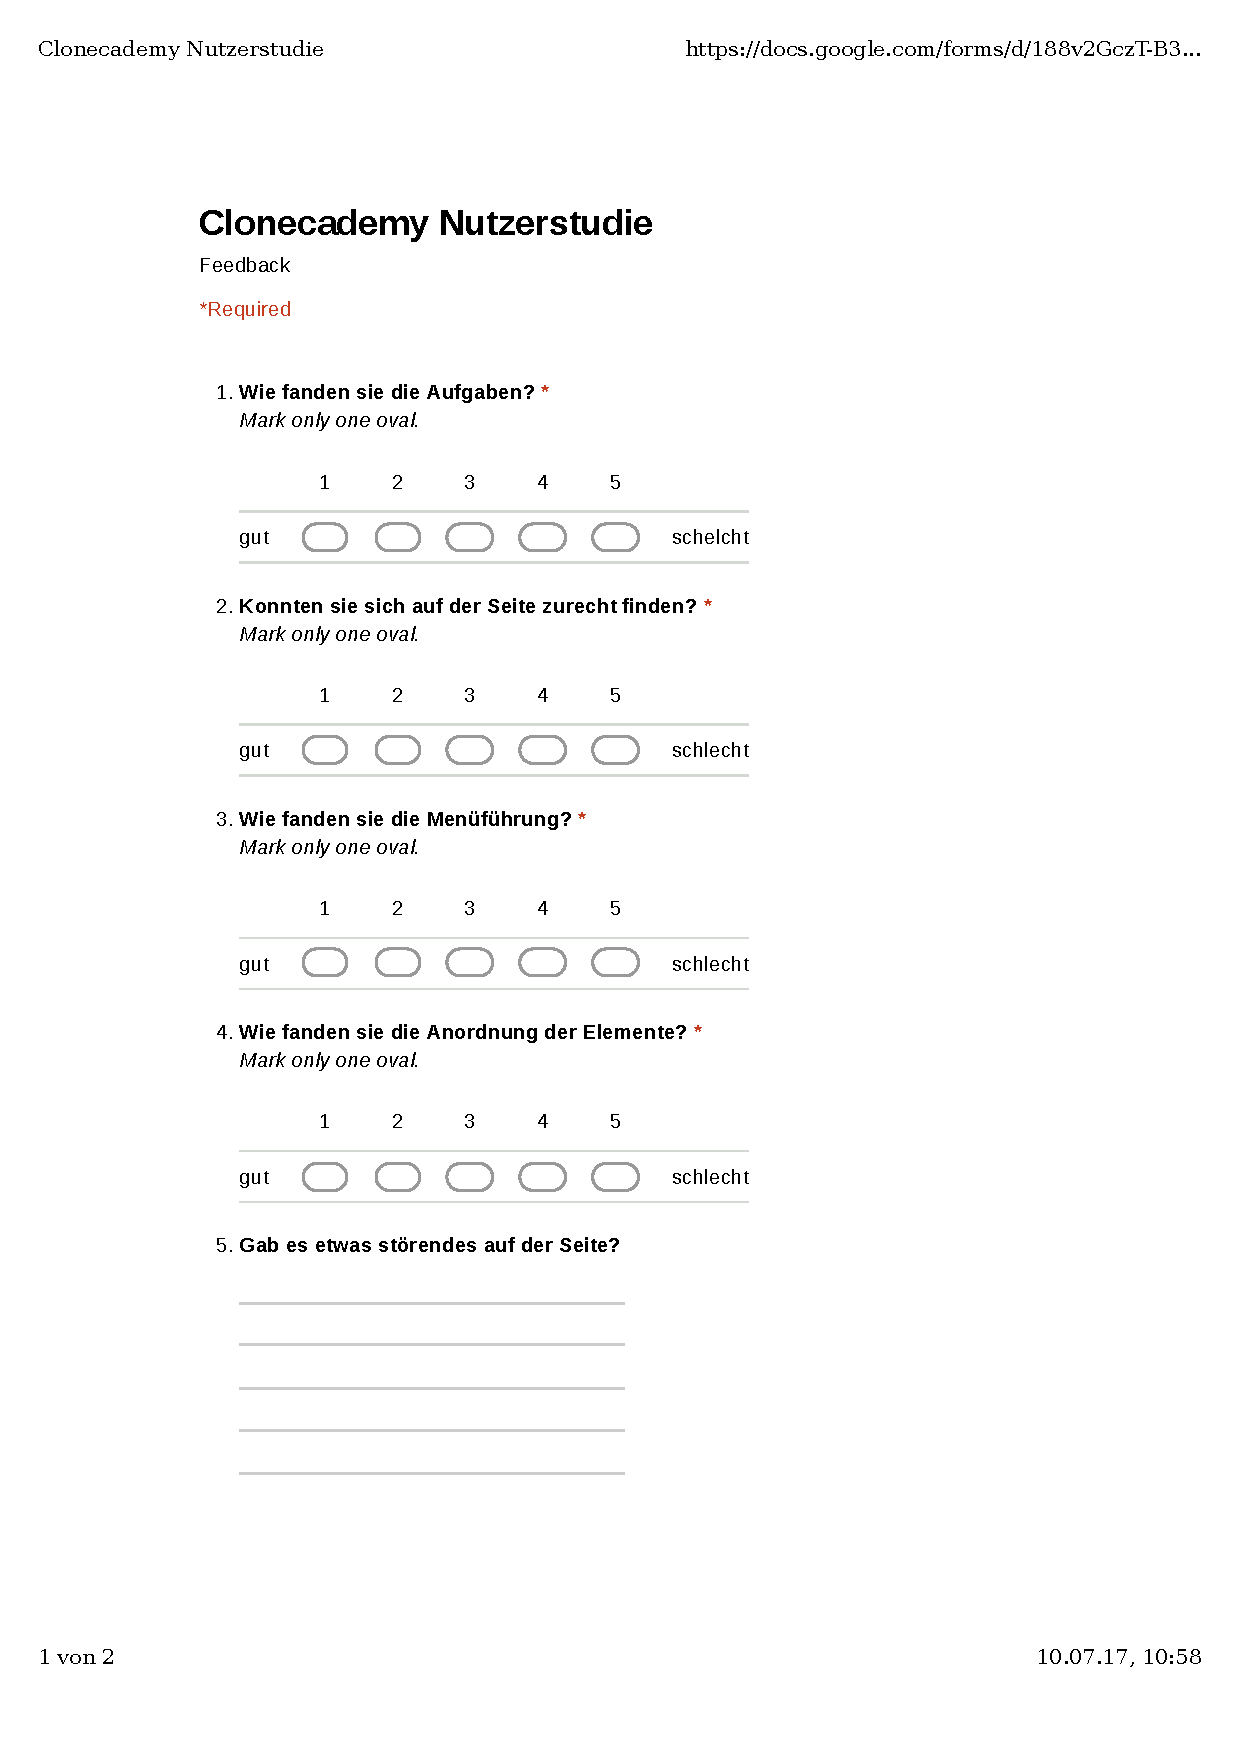
\includepdf[pages=-,pagecommand={},width=\textwidth]{nutzerstudie.pdf}


\chapter{Einleitung - Bericht und Anmerkung zum QS Prozess}
\section{Änderungen des Prozesses während des Semesters}
Während des Semesters ist dem Team aufgefallen, dass der vorgestellte QS-Prozess nicht optimal ist. Die wichtigste Änderung ist, dass die automatisiere Code-Überprüfung im Backend durch das Tool \emph{pylint} mit dem \emph{pylint\_django} Plugin durchgeführt wurde. Dieses vereinigt die Funktionen von \emph{pep8} und \emph{django-lint}, ist einfacher konfigurier- und zu verwendbar. Das Team hat deshalb beschlossen, dieses Tool zu verwenden, obwohl im QS-Dokument ein anderes vorgeschlagen wurde. Des weiteren haben wir beschlossen, im Python Backend eine Code Qualität von 9.5/10 Punkten anzustreben, da eine Behebung aller Fehler durch Eigenheiten der Tools nicht immer möglich war.

\section{Durchführung der Maßnahmen kurz vor Abgabe}
Einige QS-Maßnahmen wurden noch einmal kurz vor Abgabe des Projektes an die Auftraggeber*innen durchgeführt, auch wenn die Zeit an diesem Punkt nicht mehr ausreicht, um gefundene Probleme noch zu beheben. Dies hat den Hintergrund, dass die Auftraggeber*innen explizit wünschen, dass das Produkt auch in Zukunft noch weiter entwickelt und verfeinert wird. Somit haben wir beschlossen, einen letzten Durchlauf der Nutzungsstudien zu machen, um somit dem iGEM-Team die Möglichkeiten dazu an die Hand zu geben.

\chapter{Nachweis über den QS Prozess pro Iteration}
Um dieses Dokument nicht unübersichtlich werden zu lassen, wurden nicht alle Outputs der automatisierten Tests angehängt. Wir haben stattdessen die Meldungen zum Stand der wöchentlichen Abgabe gespeichert, um den Verlauf der Softwareentwicklung deutlich zu machen.

Bei den Berichten über die Testabdeckung haben wir zu jeder Iteration die Übersichtsseite der Reports angehängt, und einen gesamten Report für das finale Produkt.

Um die Dokumentation der Webseite im Wiki anschaulich zu dokumentieren, haben wir das gesamte Wiki bei Stand der Abgabe angehängt. Eine Rekonstruktion des Stands der jeweiligen Releases ist leider wegen der fehlenden Versionsgeschichte der Github Integration nicht mehr möglich.

Die Dokumentation zum QS-Ziel ''Bedienbarkeit'' anschaulich zu gestalten, haben wir die Veränderungen an der Webseite durch Screenshots dokumentiert. Zusätzlich finden sich die Checklisten (pro Iteration) und die aus den Nutzungsstudien entstandenen Dokumente (Protokolle und Issues in GitHub) im folgenden Anhang.

\section*{Iteration 7 - 29.06.}
	Wir haben unseren QS-Prozess das erste Mal zur 7. Iteration durchgeführt, allerdings noch nicht vollständig (einige Details fehlen noch, z.B. geänderte Tools). Um den Stand der Software vor Beginn des Prozesses zu dokumentieren, haben wir alle QS-Maßnahmen am Produkt durchgeführt, ohne etwas an der Software zu ändern. Das bietet uns die Basis für den weiteren Verlauf.
	
	Abgegebene Userstories (bislang): 1, 2, 3, 5, 6, 7, 8, 9, 10, 11, 14, 15, 16
	
	Commit Hash der ersten Durchführung: 22f76fcce2d1d6b03857a9a4db7f9276433aecdd
	
	\subsection{Checklisten}
	
	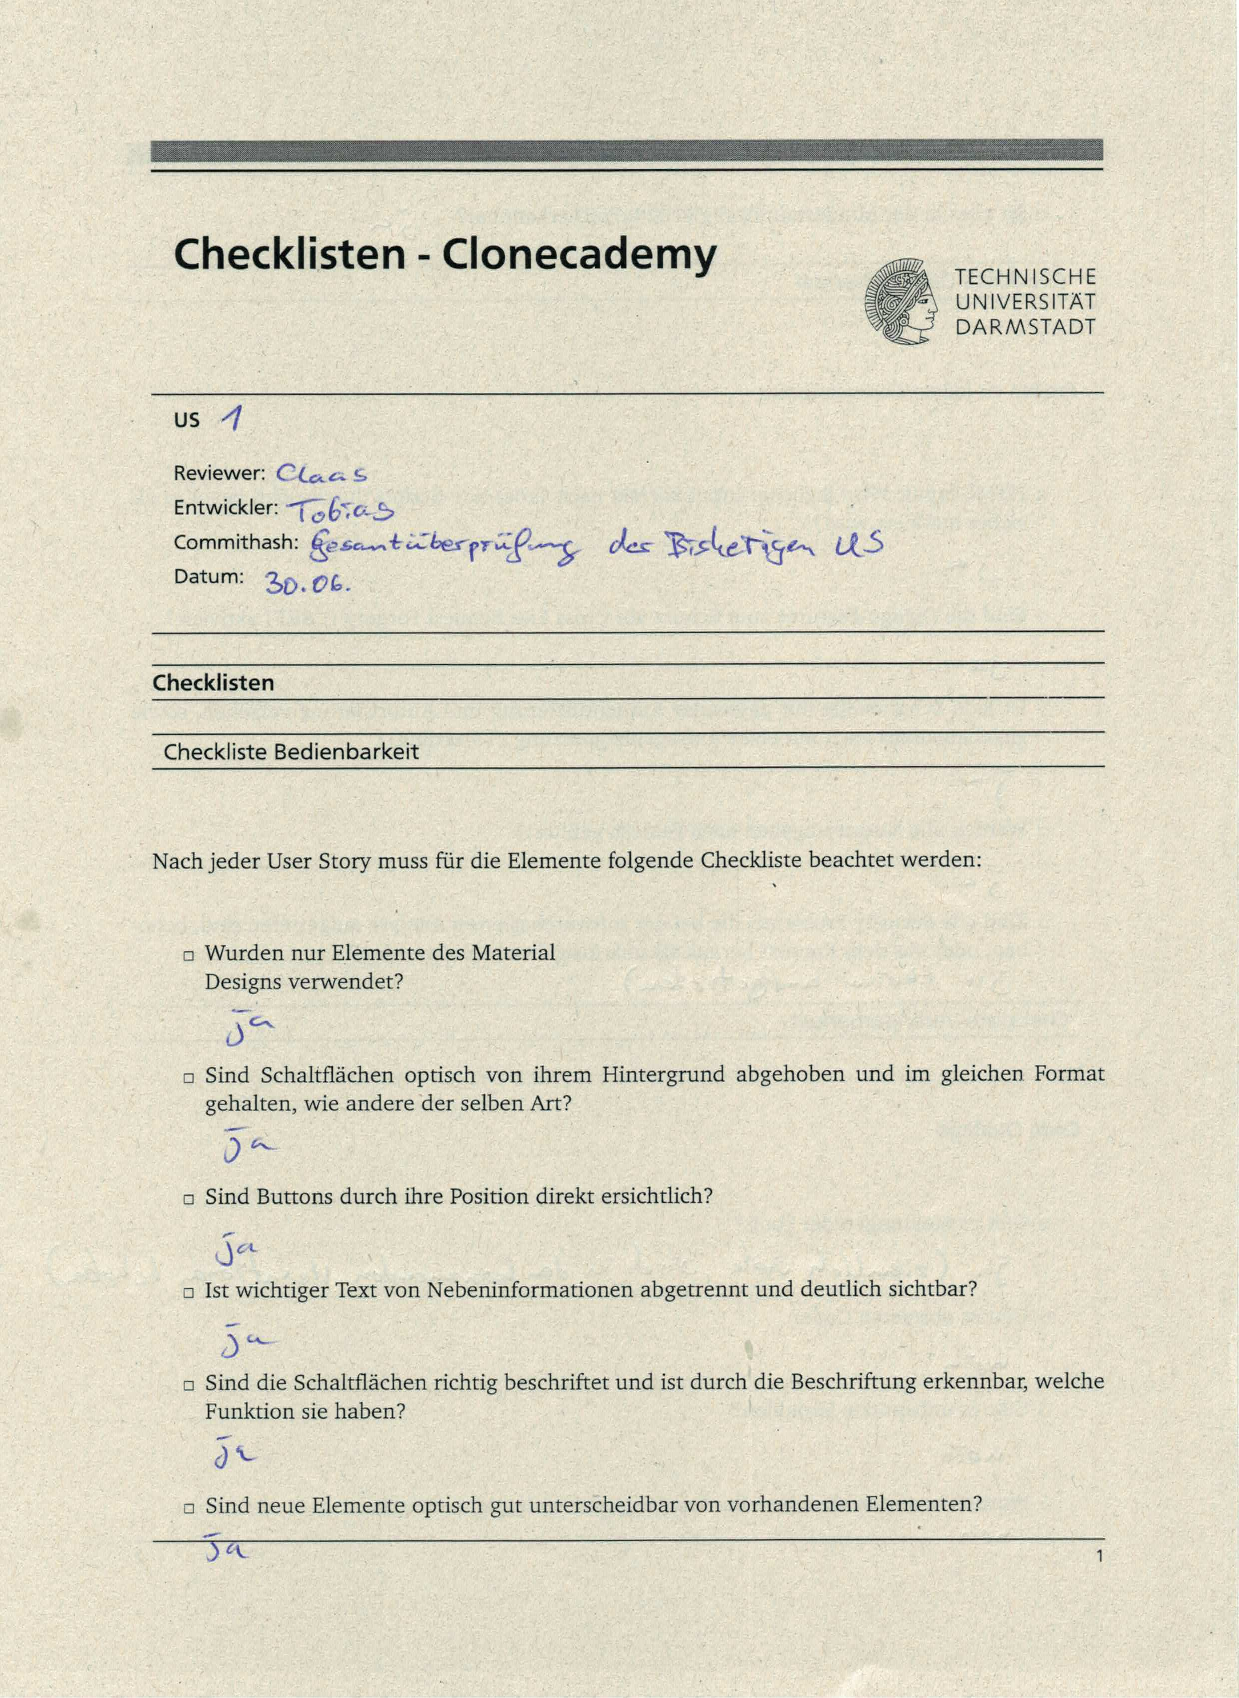
\includepdf[pages=-,pagecommand={},width=\textwidth]{appendix/checklisten/01_01.pdf}
	%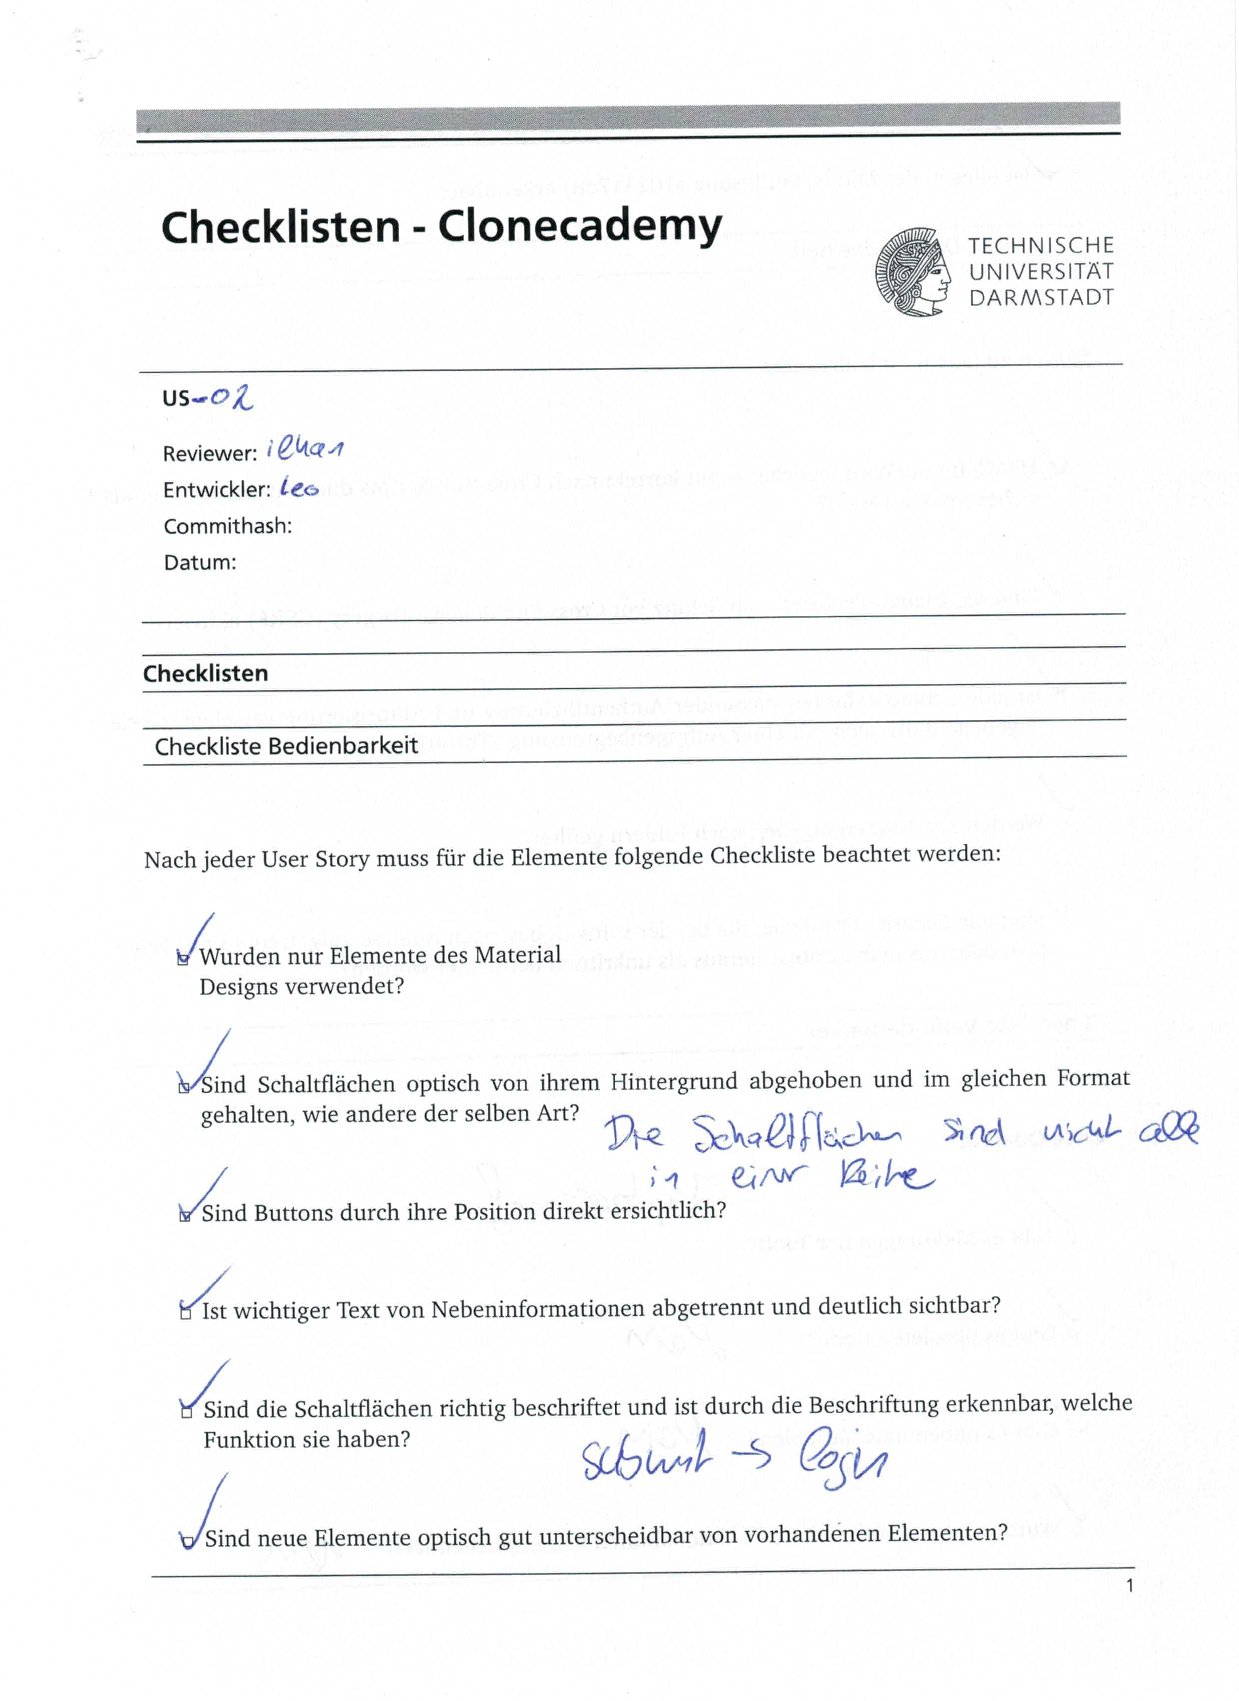
\includepdf[pages=-,pagecommand={},width=\textwidth]{appendix/checklisten/02_01.pdf}
	%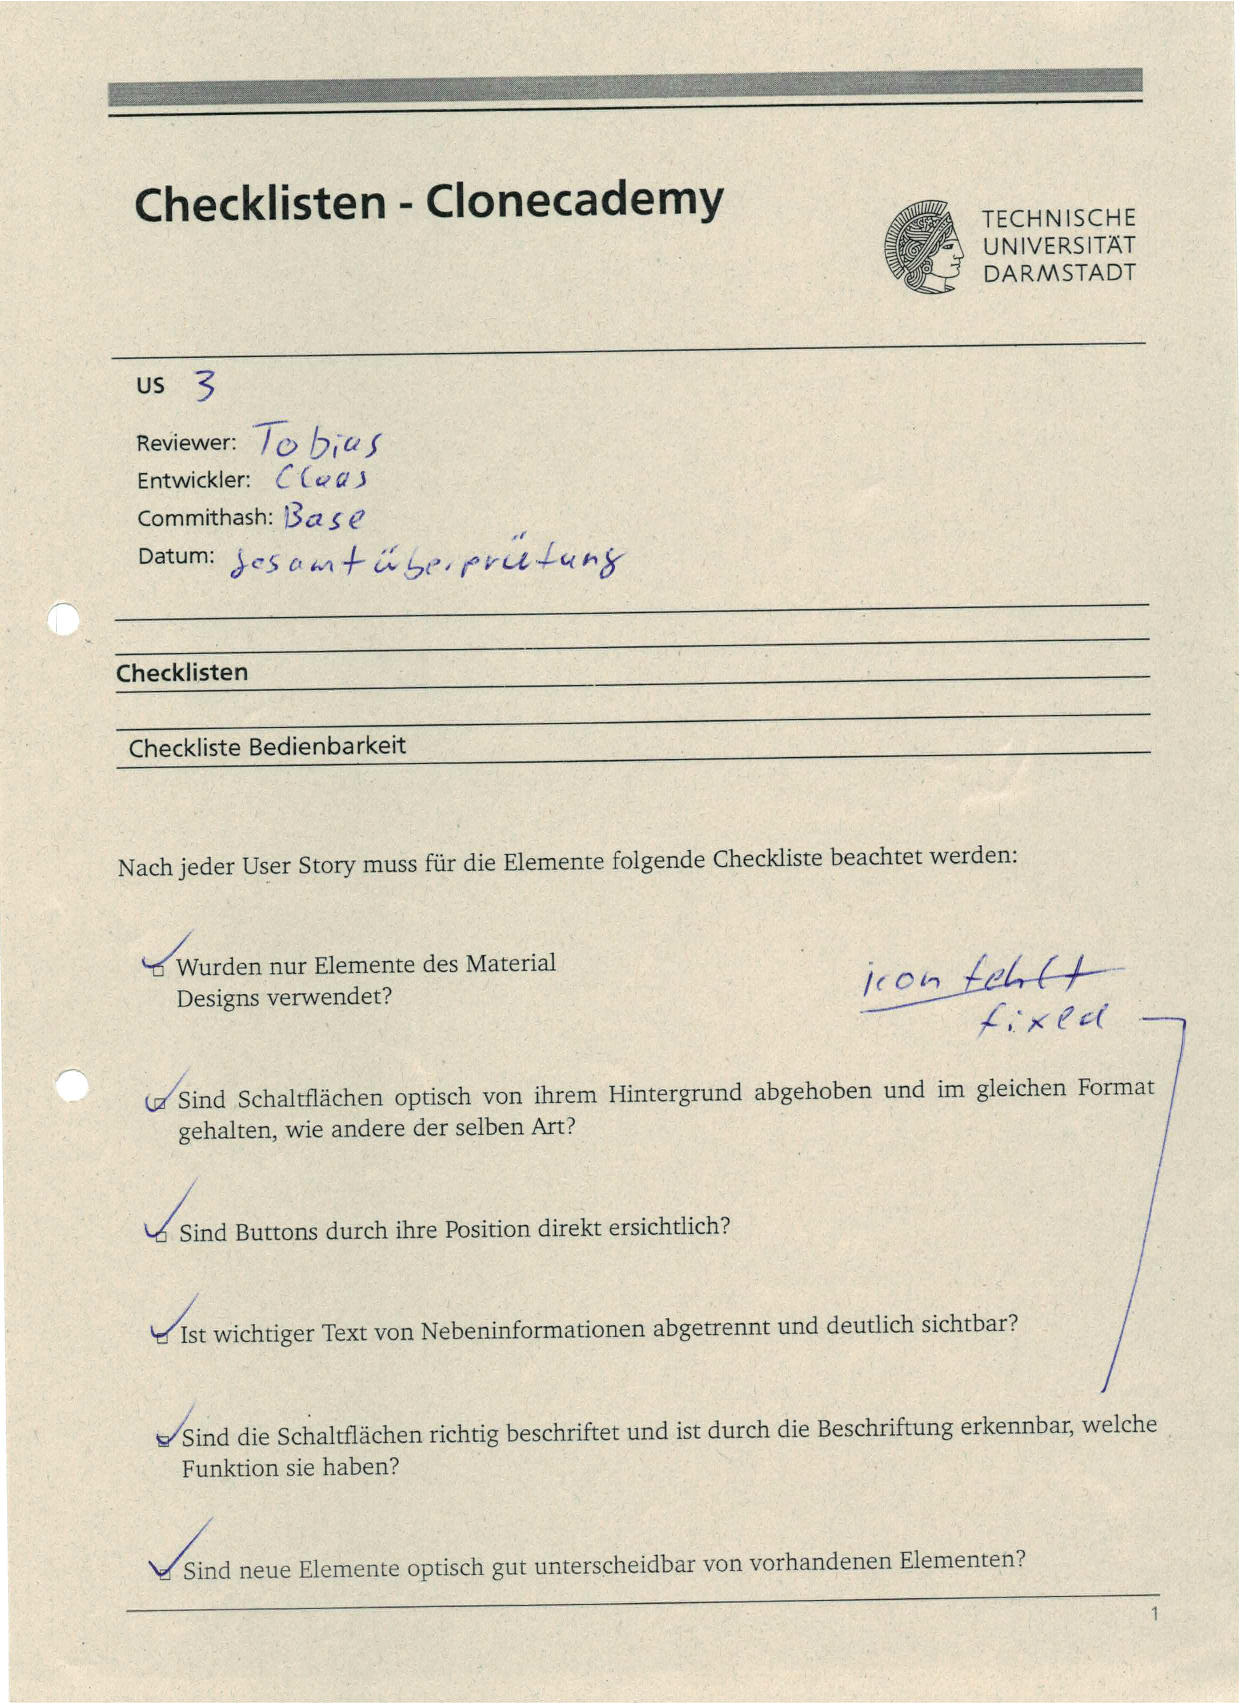
\includepdf[pages=-,pagecommand={},width=\textwidth]{appendix/checklisten/03_01.pdf}
	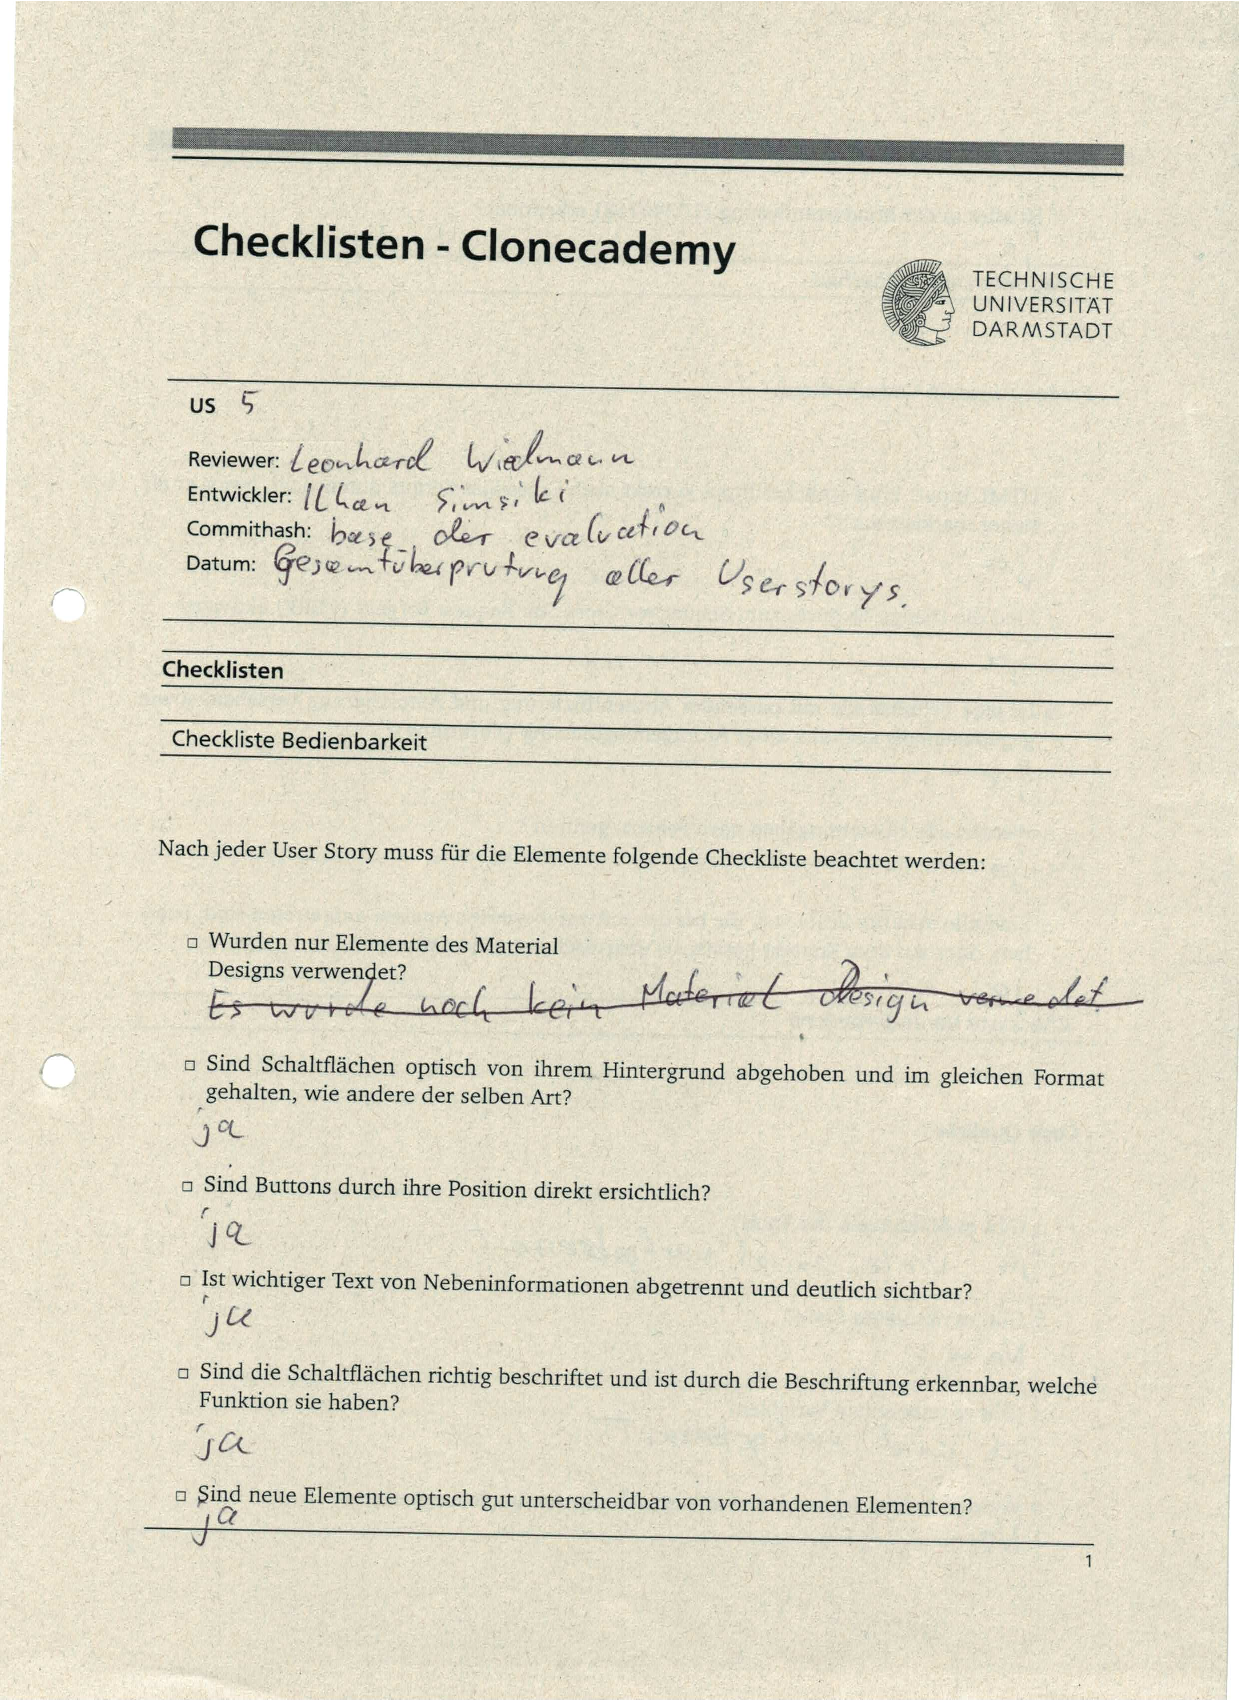
\includepdf[pages=-,pagecommand={},width=\textwidth]{appendix/checklisten/05_01.pdf}
	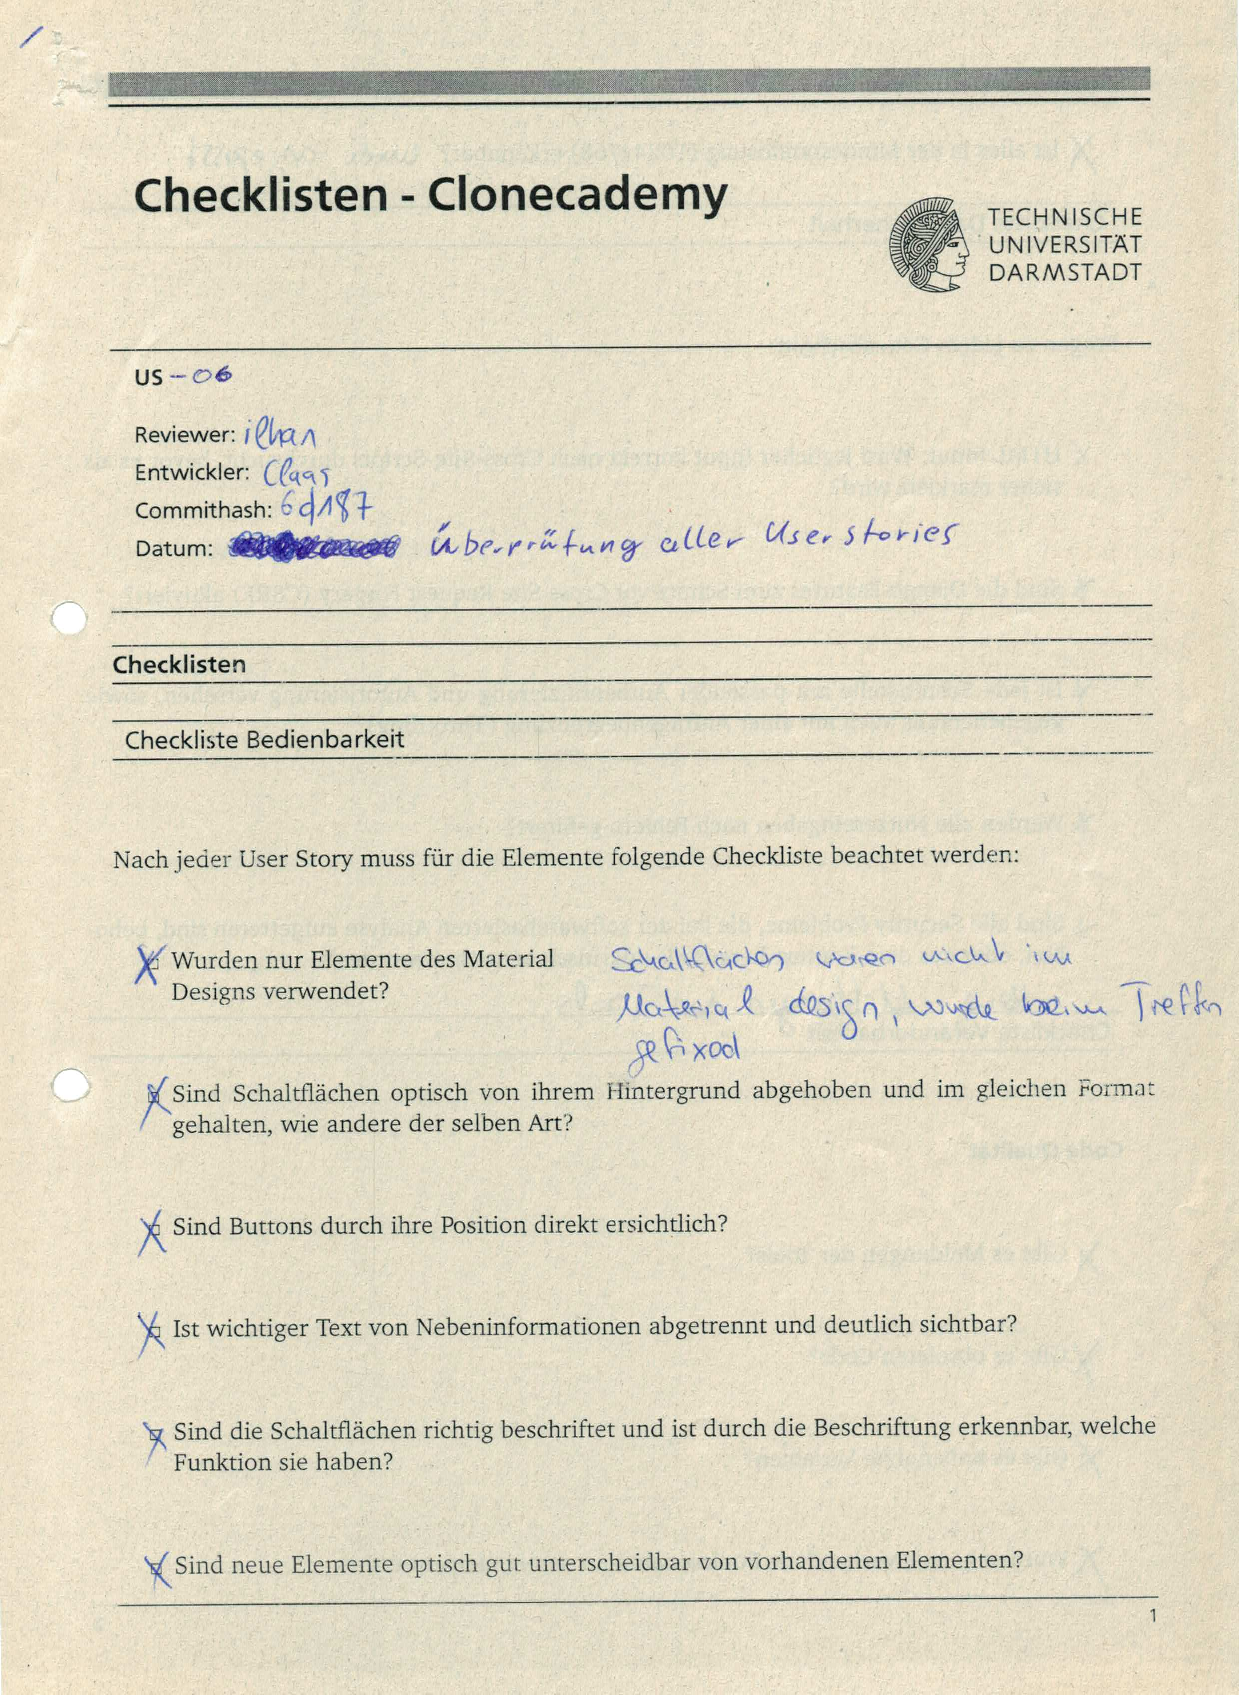
\includepdf[pages=-,pagecommand={},width=\textwidth]{appendix/checklisten/06_01.pdf}
	%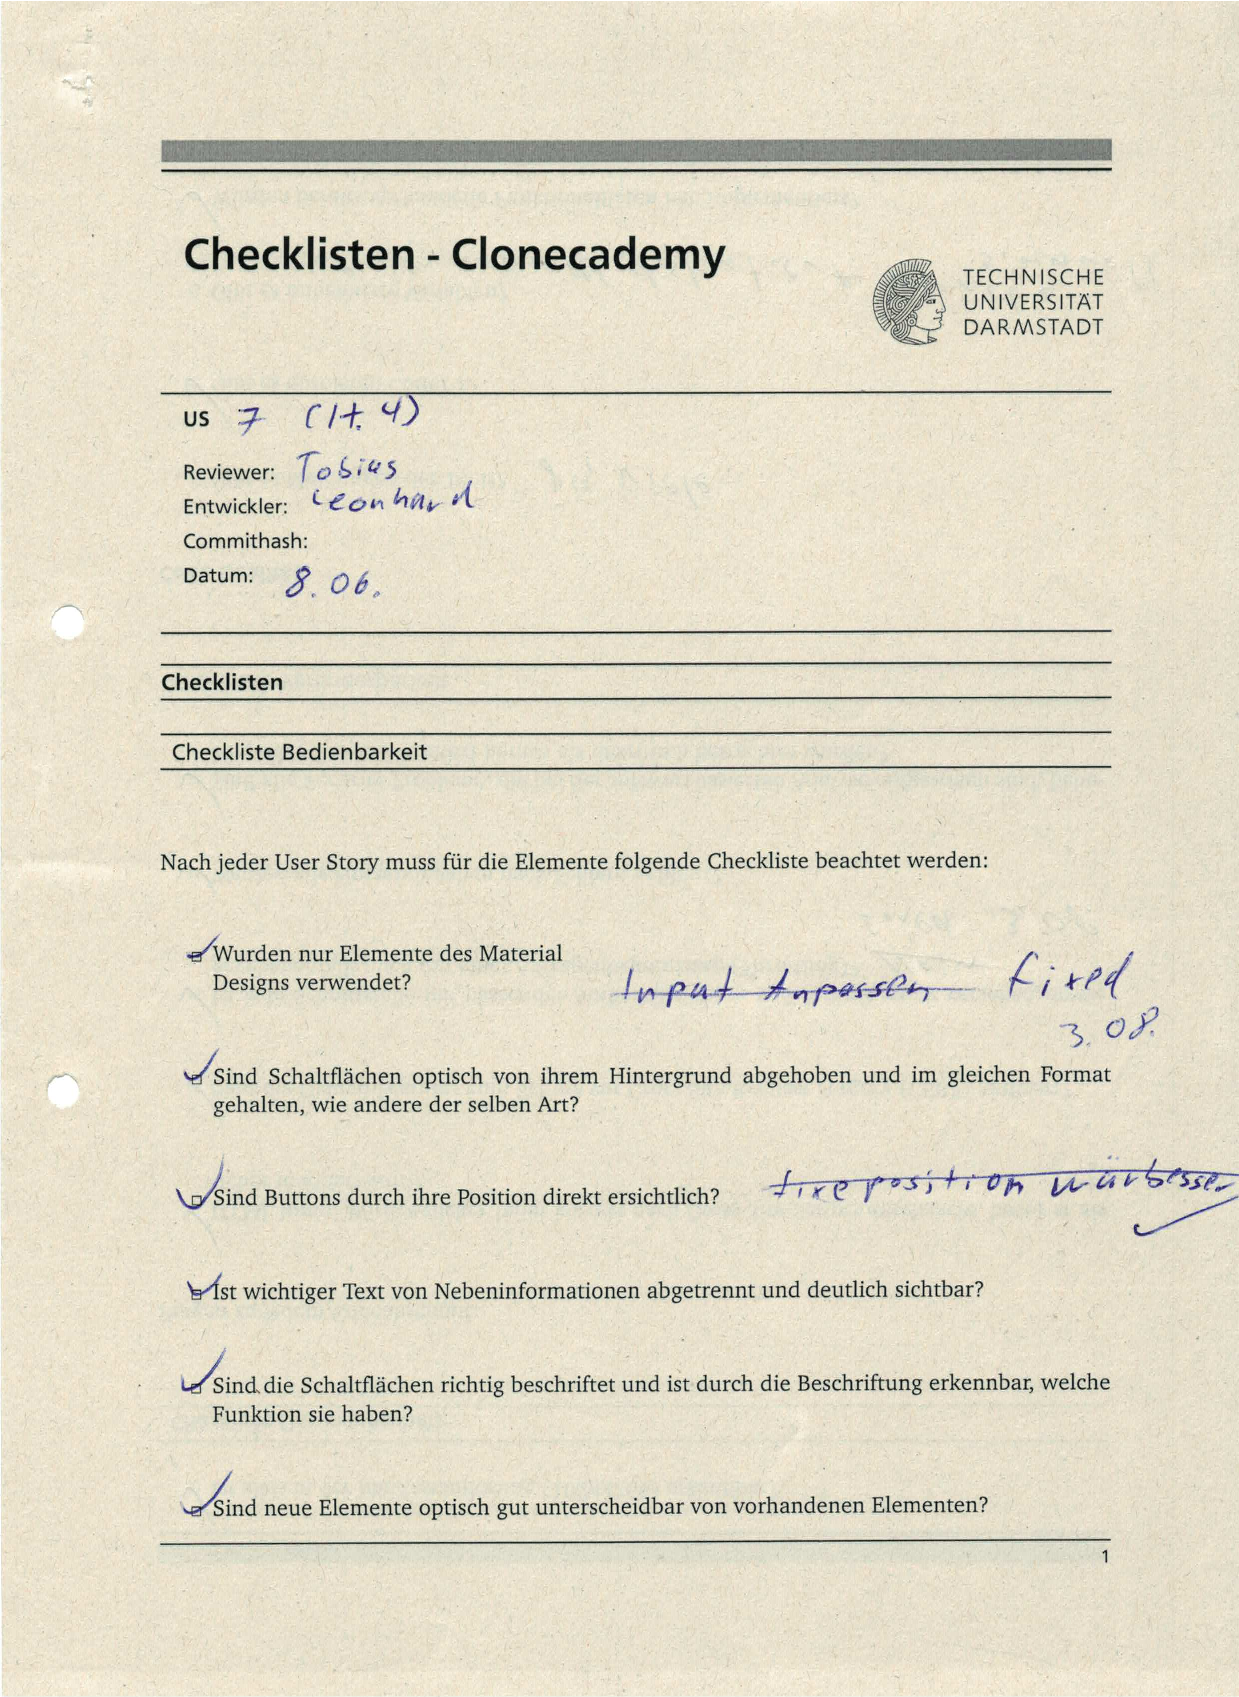
\includepdf[pages=-,pagecommand={},width=\textwidth]{appendix/checklisten/07_01.pdf}
	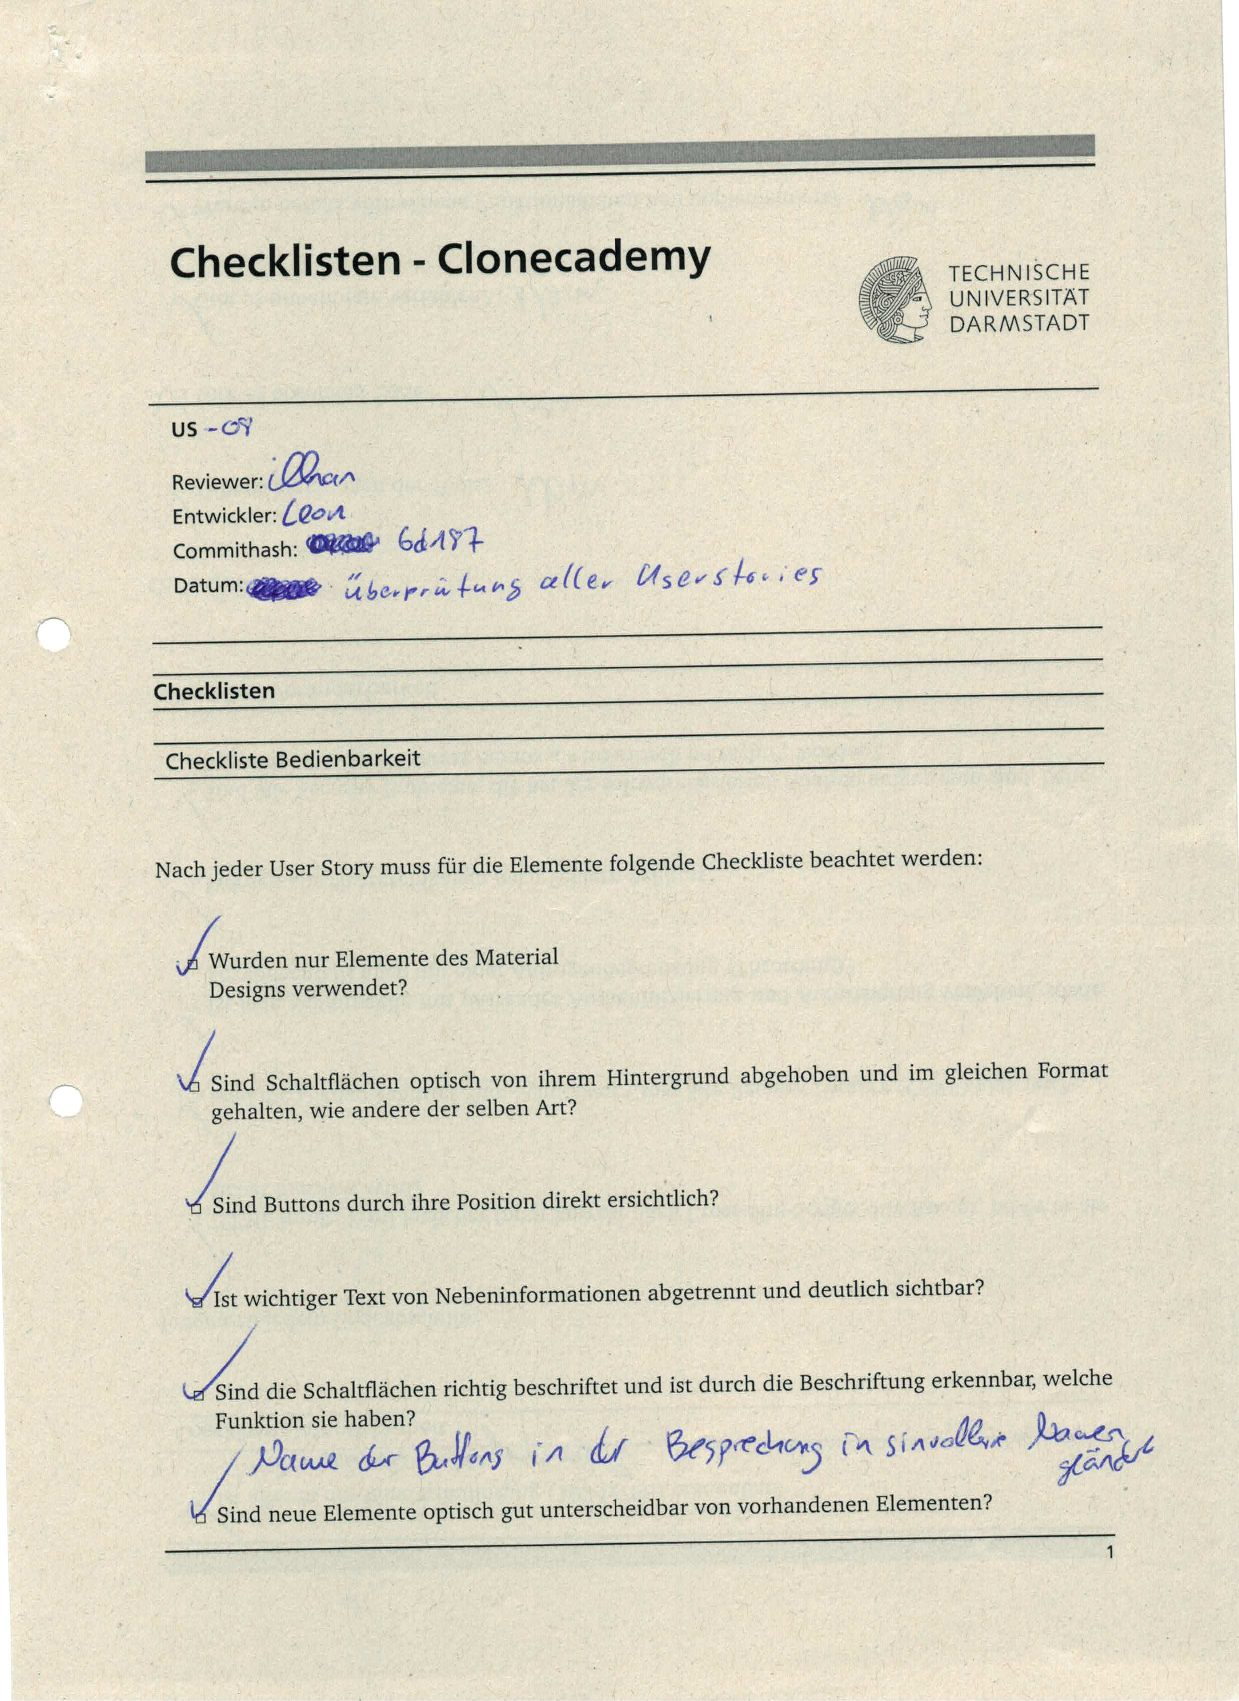
\includepdf[pages=-,pagecommand={},width=\textwidth]{appendix/checklisten/08_01.pdf}
	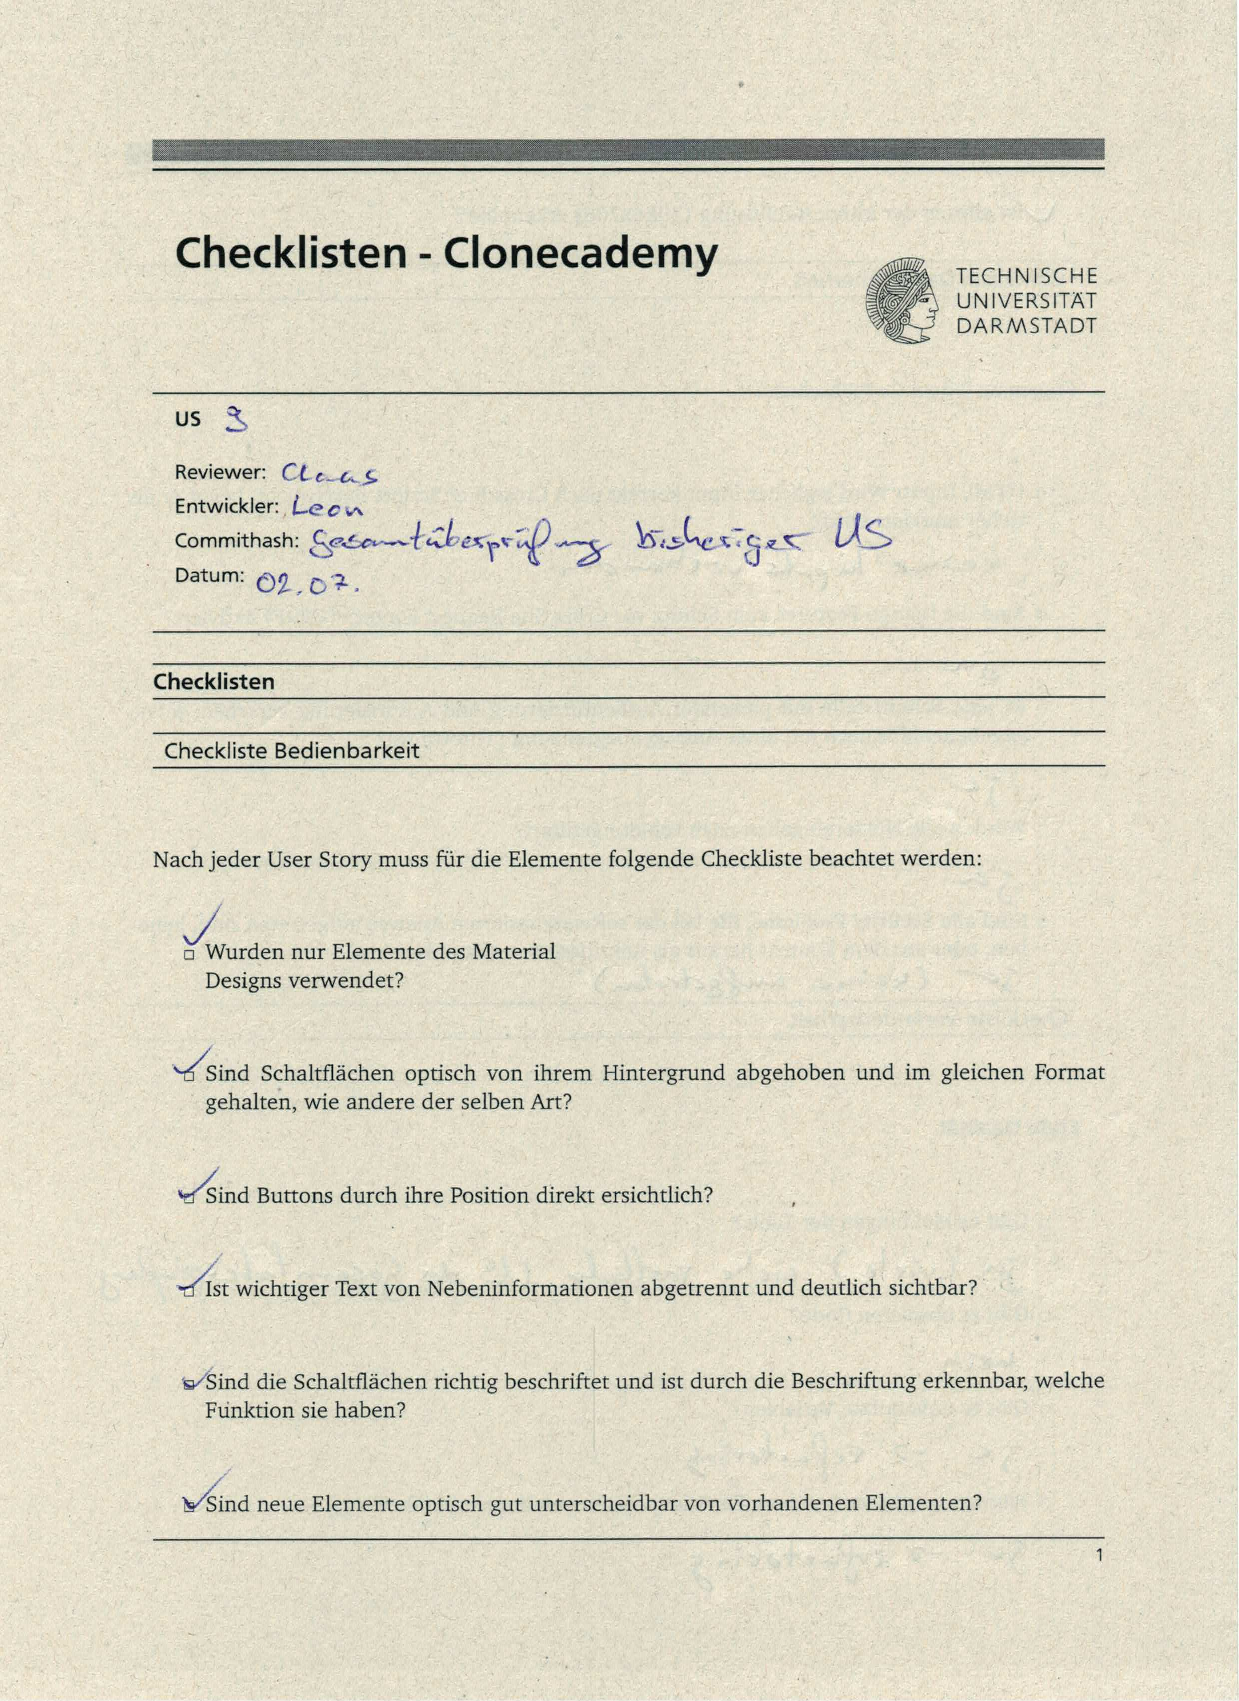
\includepdf[pages=-,pagecommand={},width=\textwidth]{appendix/checklisten/09_01.pdf}
	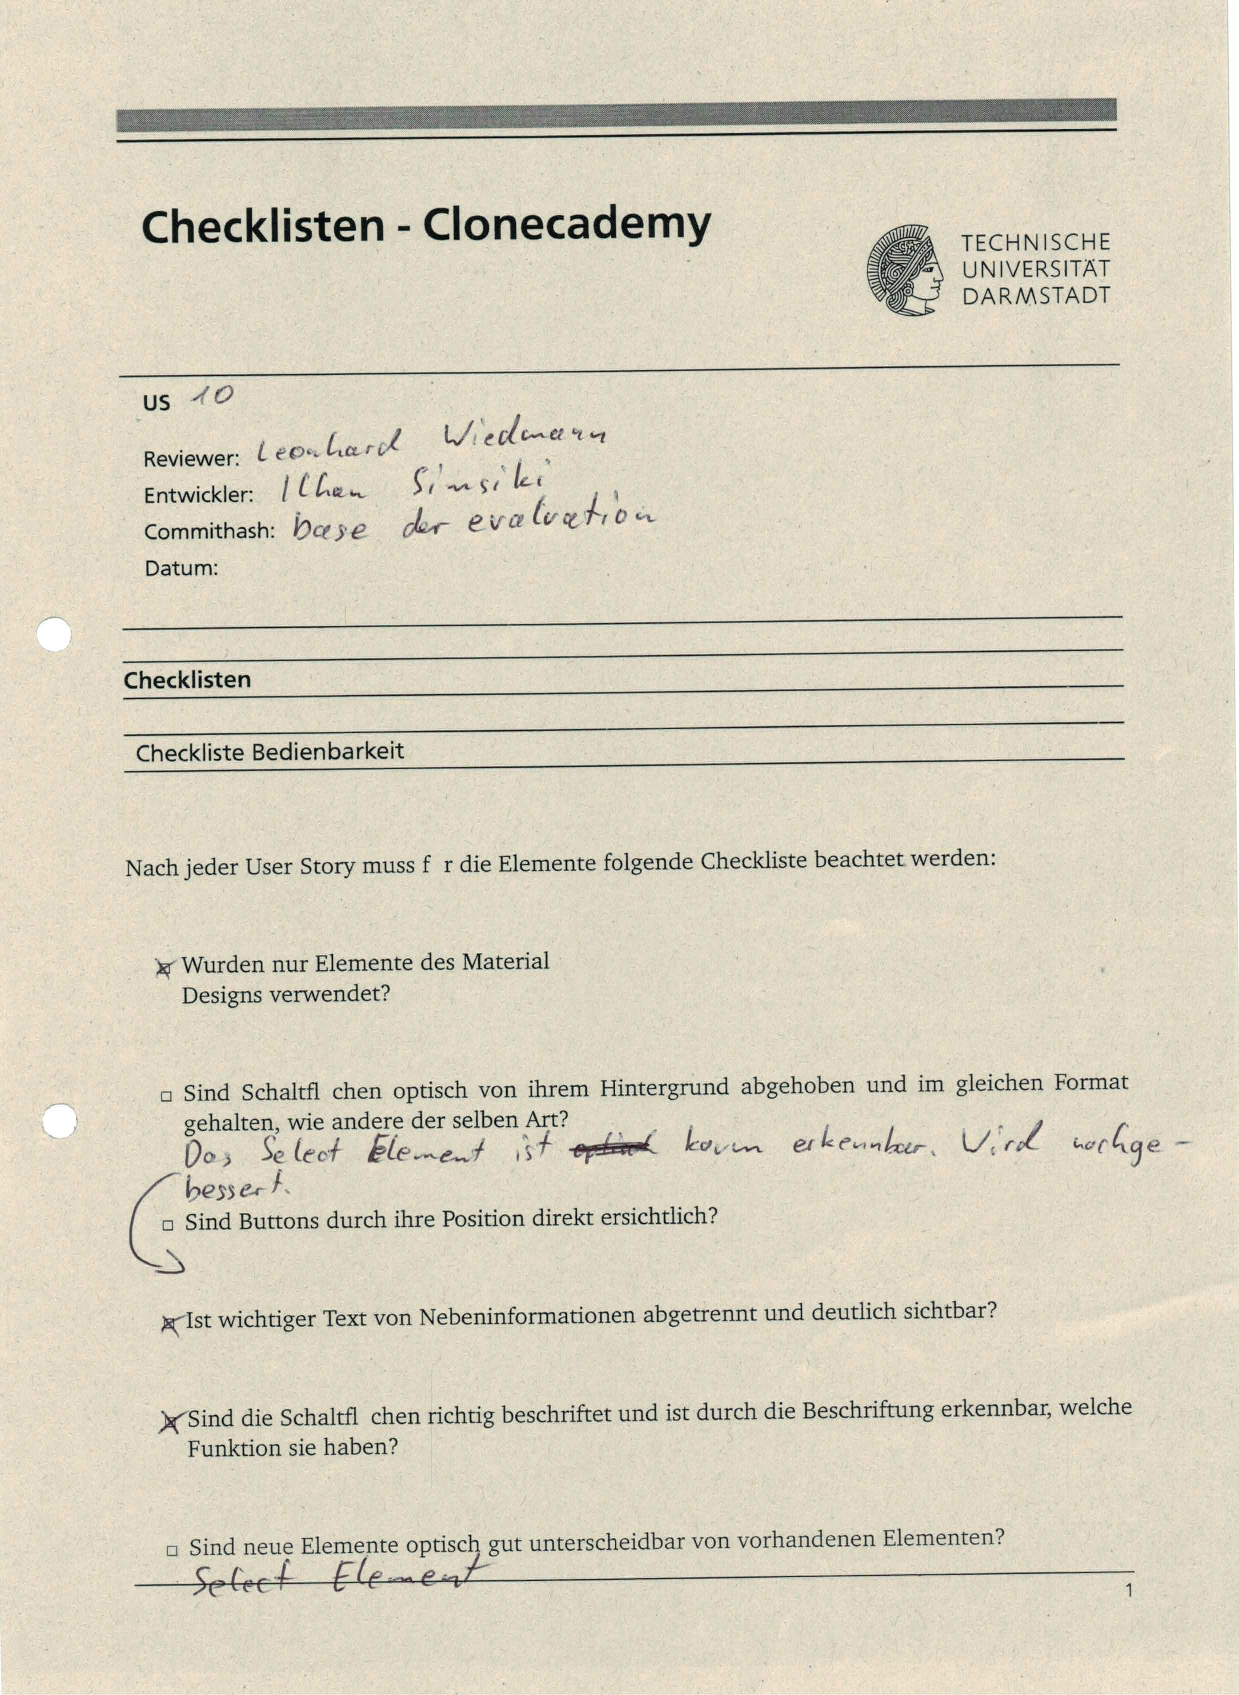
\includepdf[pages=-,pagecommand={},width=\textwidth]{appendix/checklisten/10_01.pdf}
	%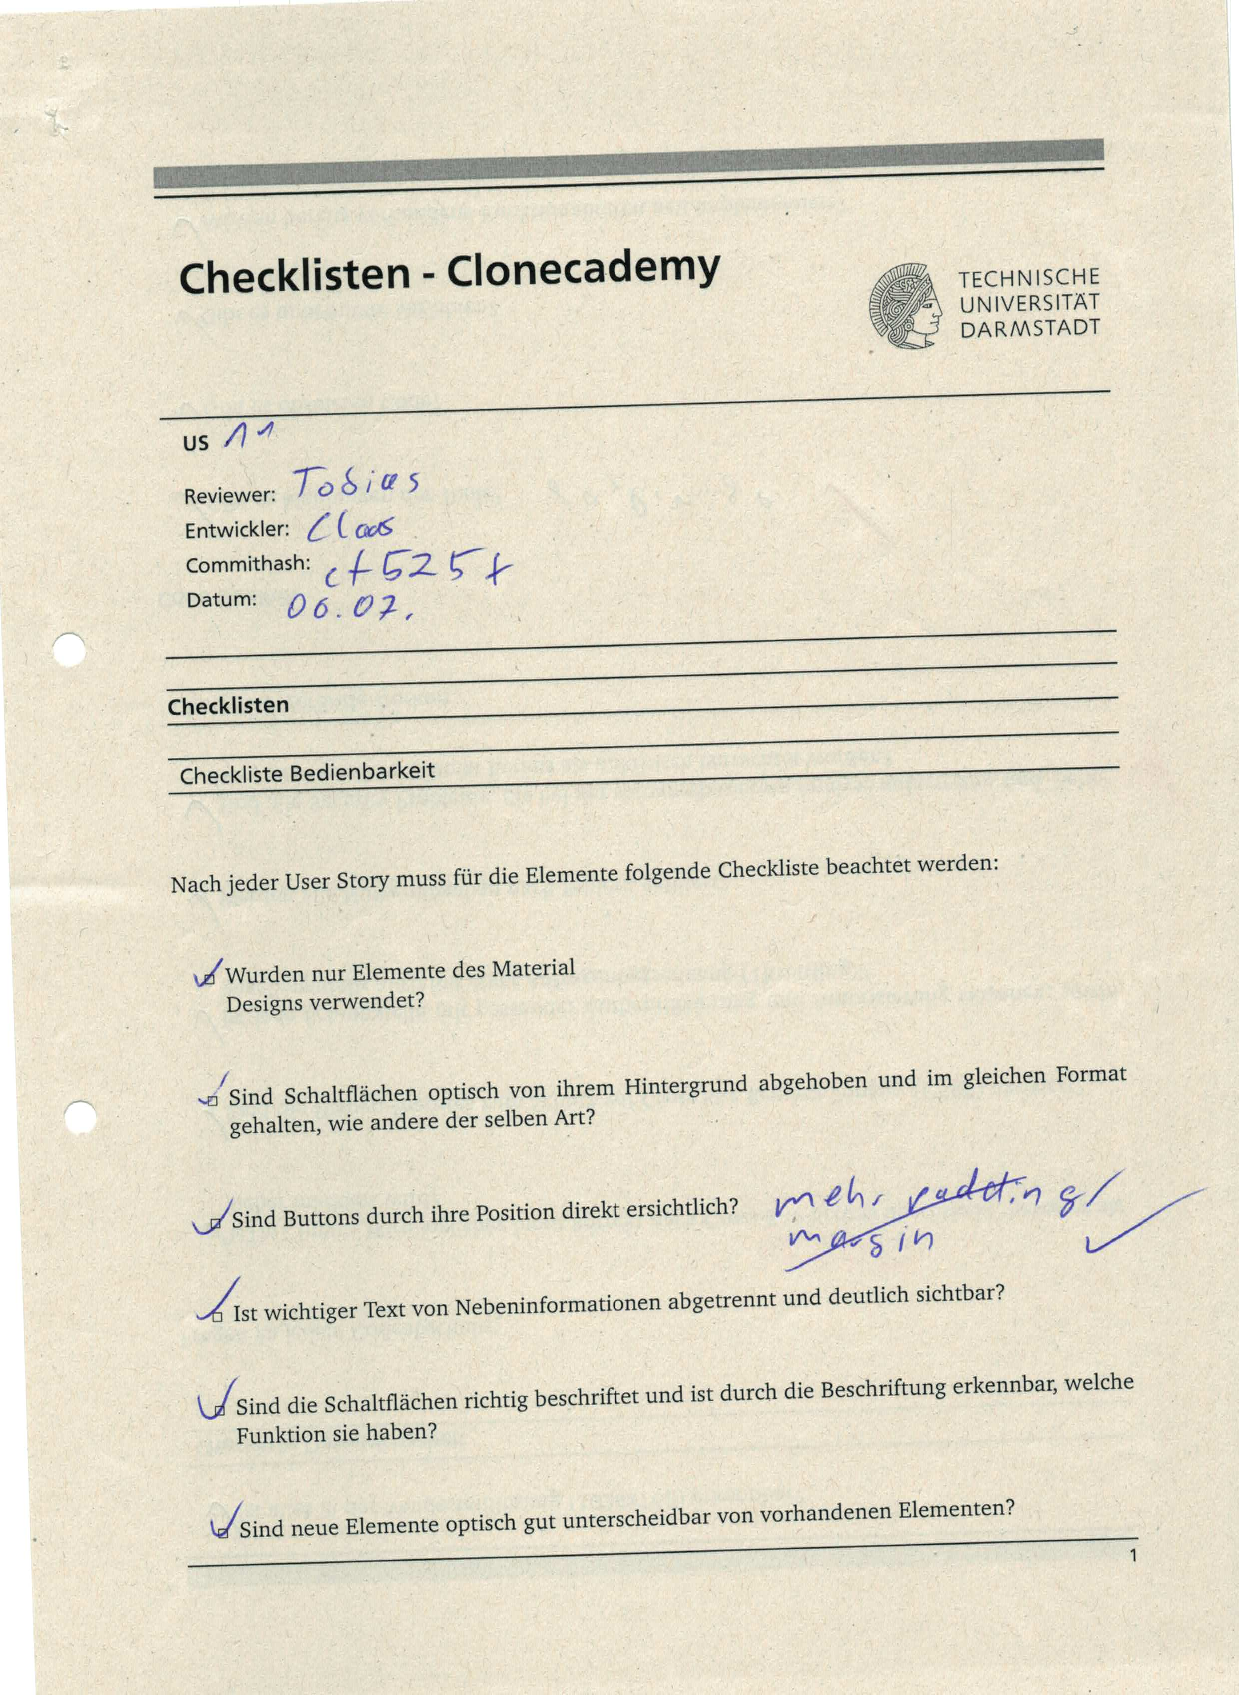
\includepdf[pages=-,pagecommand={},width=\textwidth]{appendix/checklisten/11_01.pdf}
	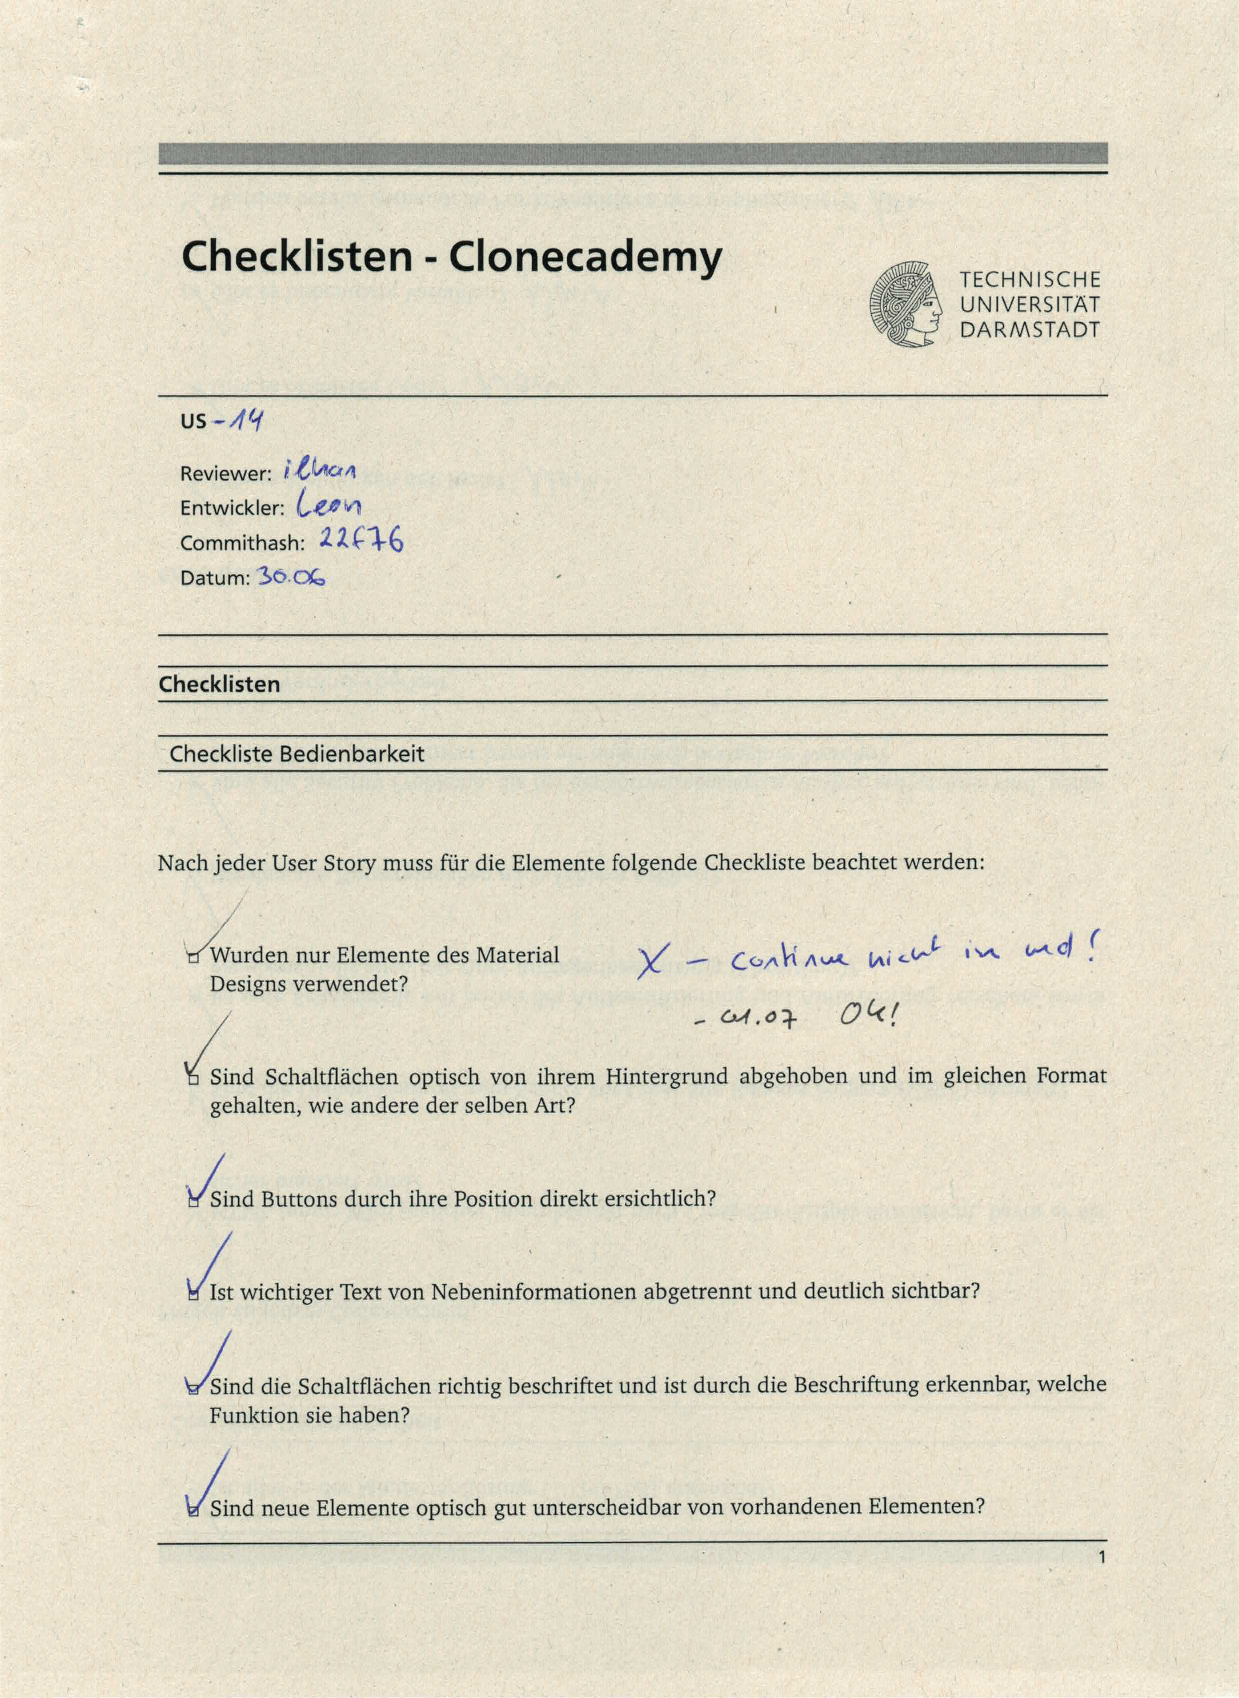
\includepdf[pages=-,pagecommand={},width=\textwidth]{appendix/checklisten/14_01.pdf}
	%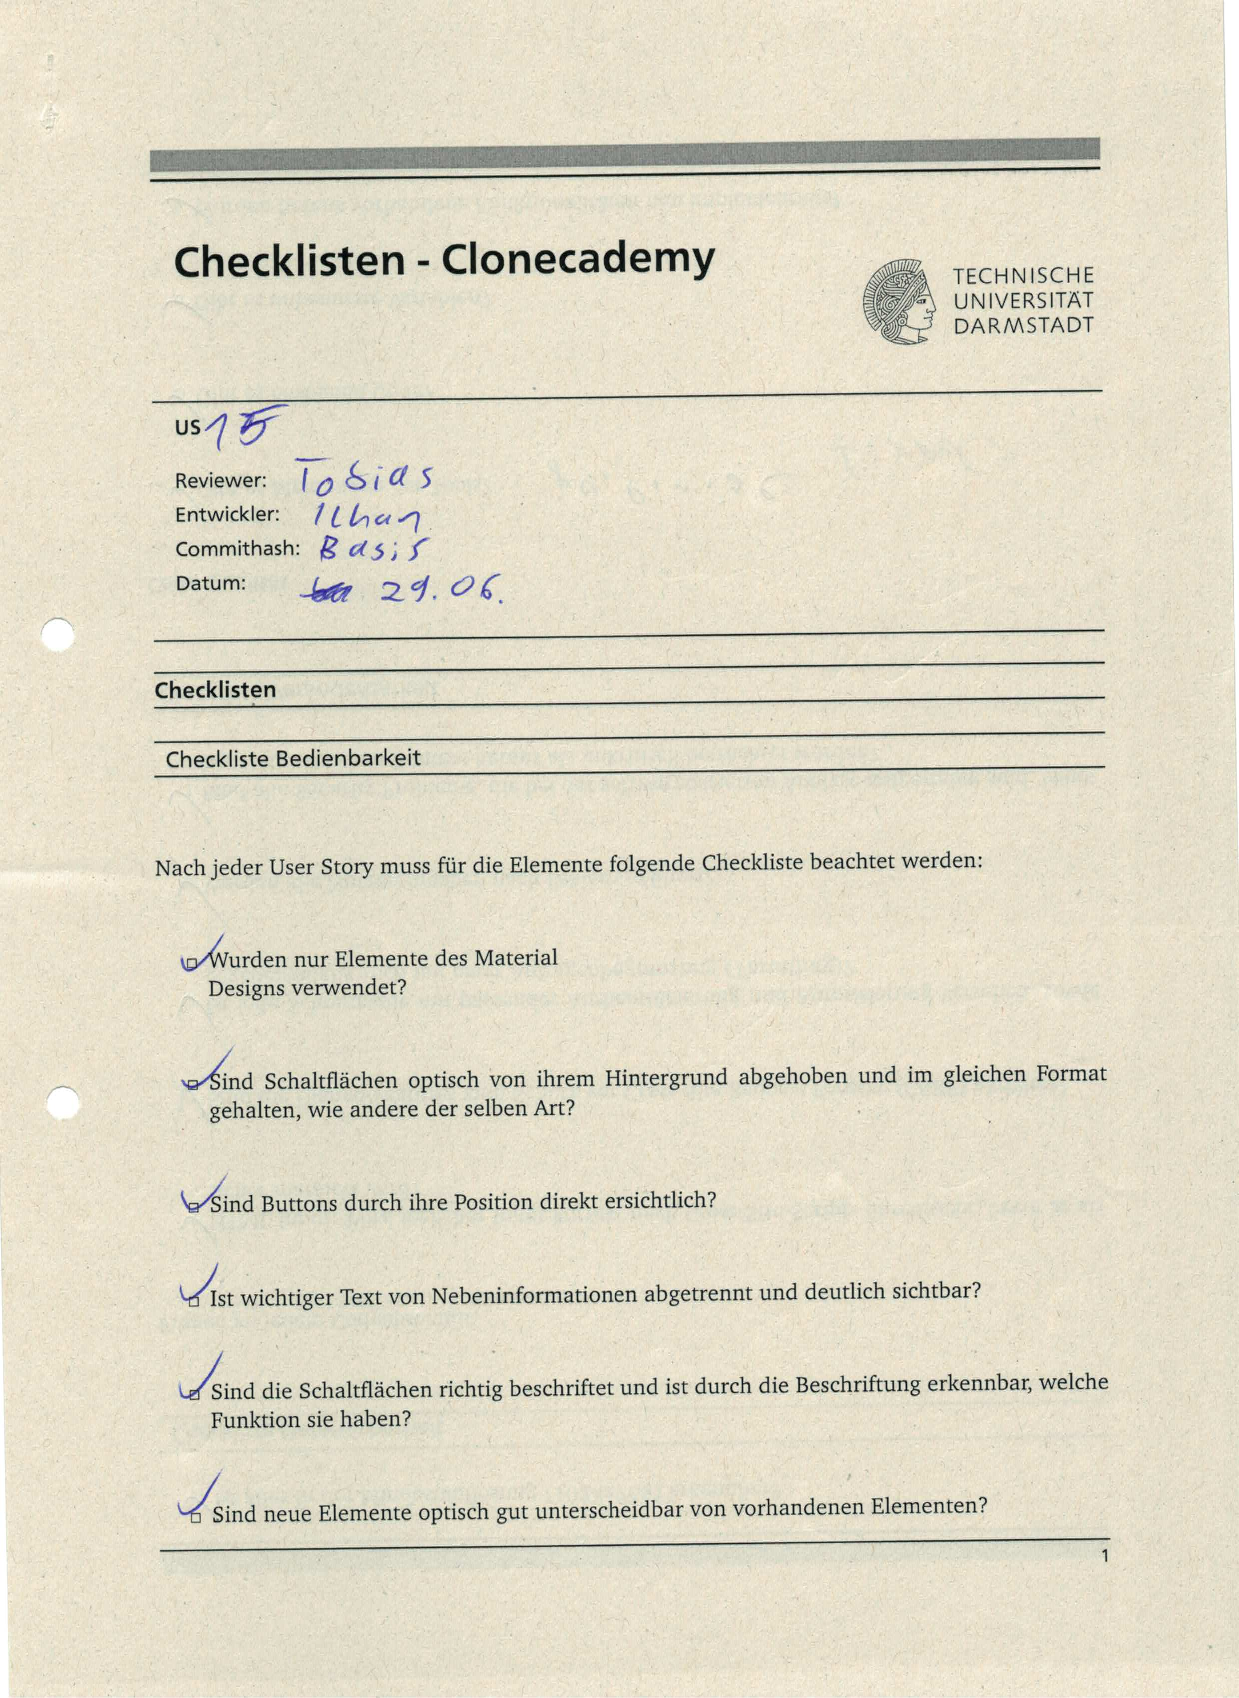
\includepdf[pages=-,pagecommand={},width=\textwidth]{appendix/checklisten/15_01.pdf}
	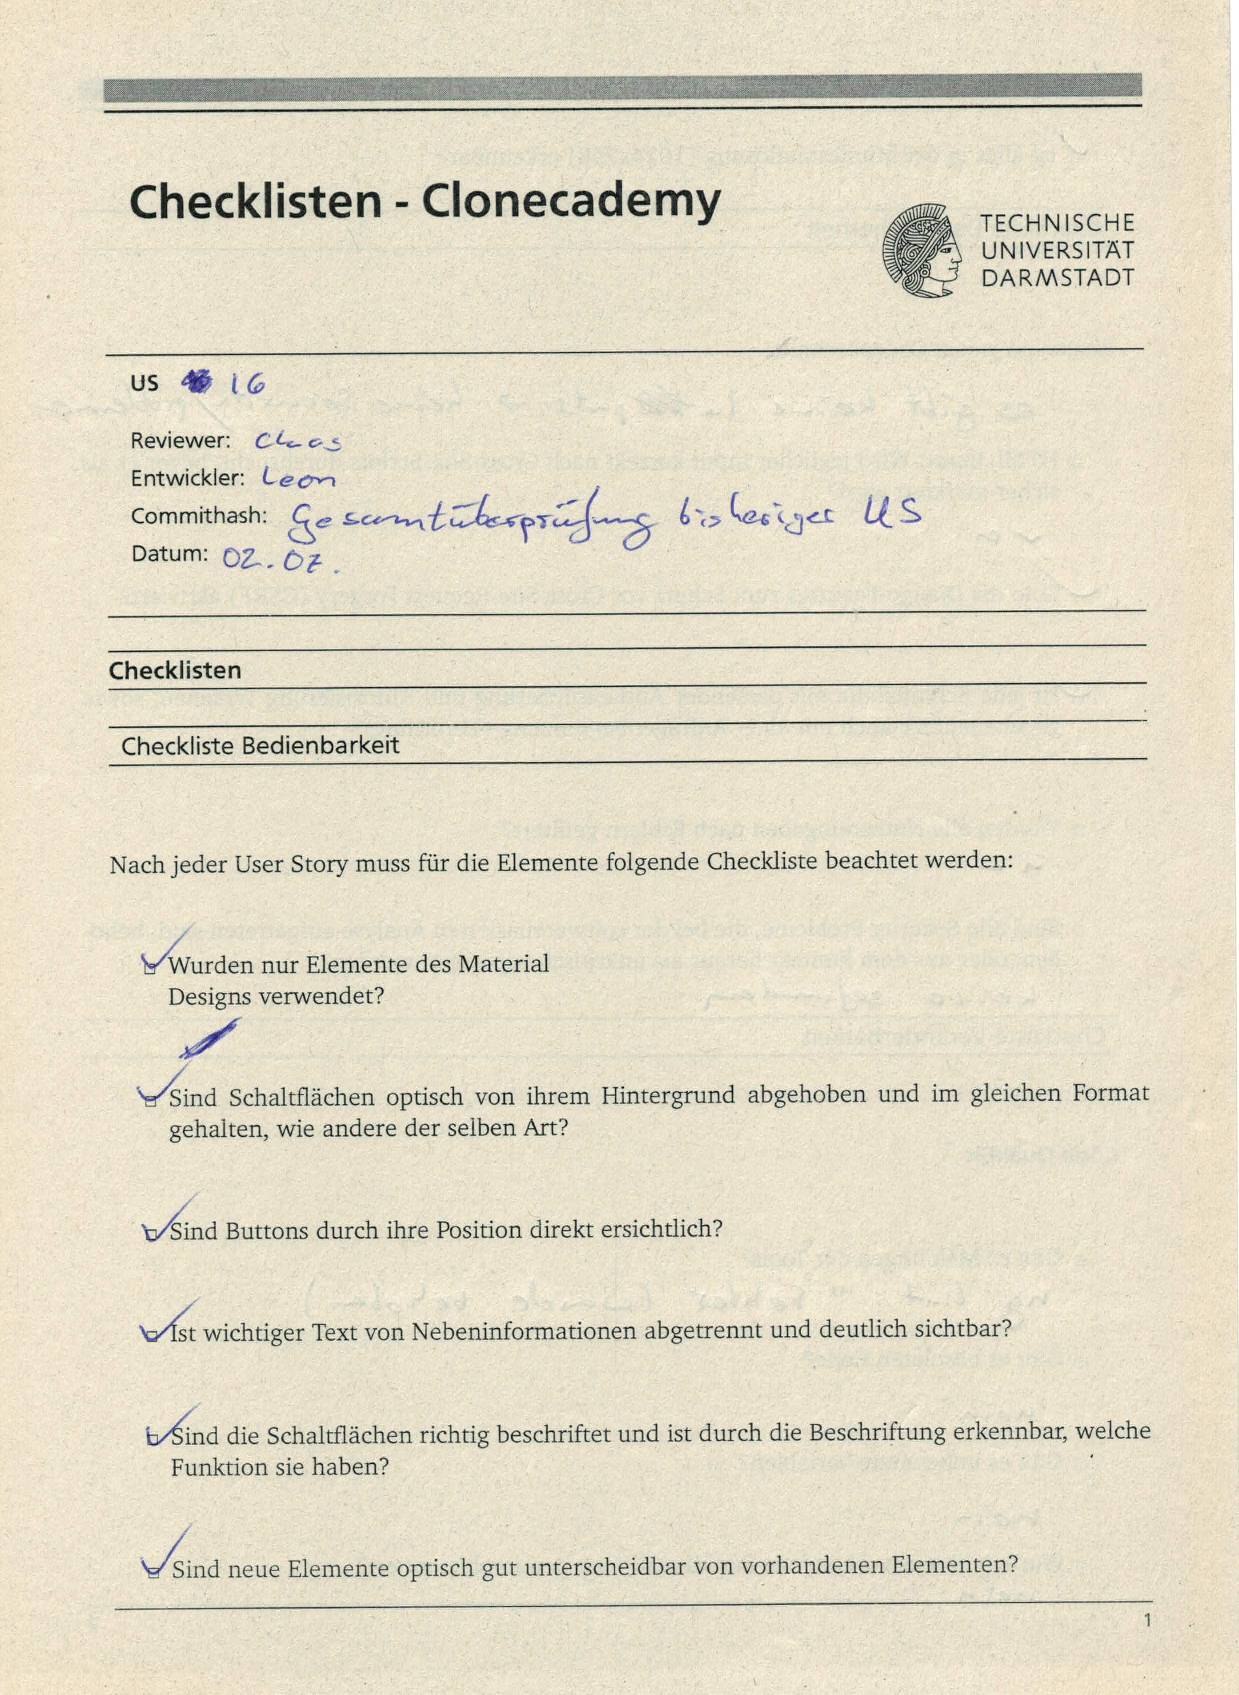
\includepdf[pages=-,pagecommand={},width=\textwidth]{appendix/checklisten/16_01.pdf}
	
	\subsection{Veränderbarkeit}
	\subsubsection{ng lint Output}
	\lstinputlisting{appendix/ng_lint/ng_clean_7.txt}

	\subsubsection{pep8 Output}
	\lstinputlisting{appendix/pep8_07.txt}

	\subsection*{coverage Output}
	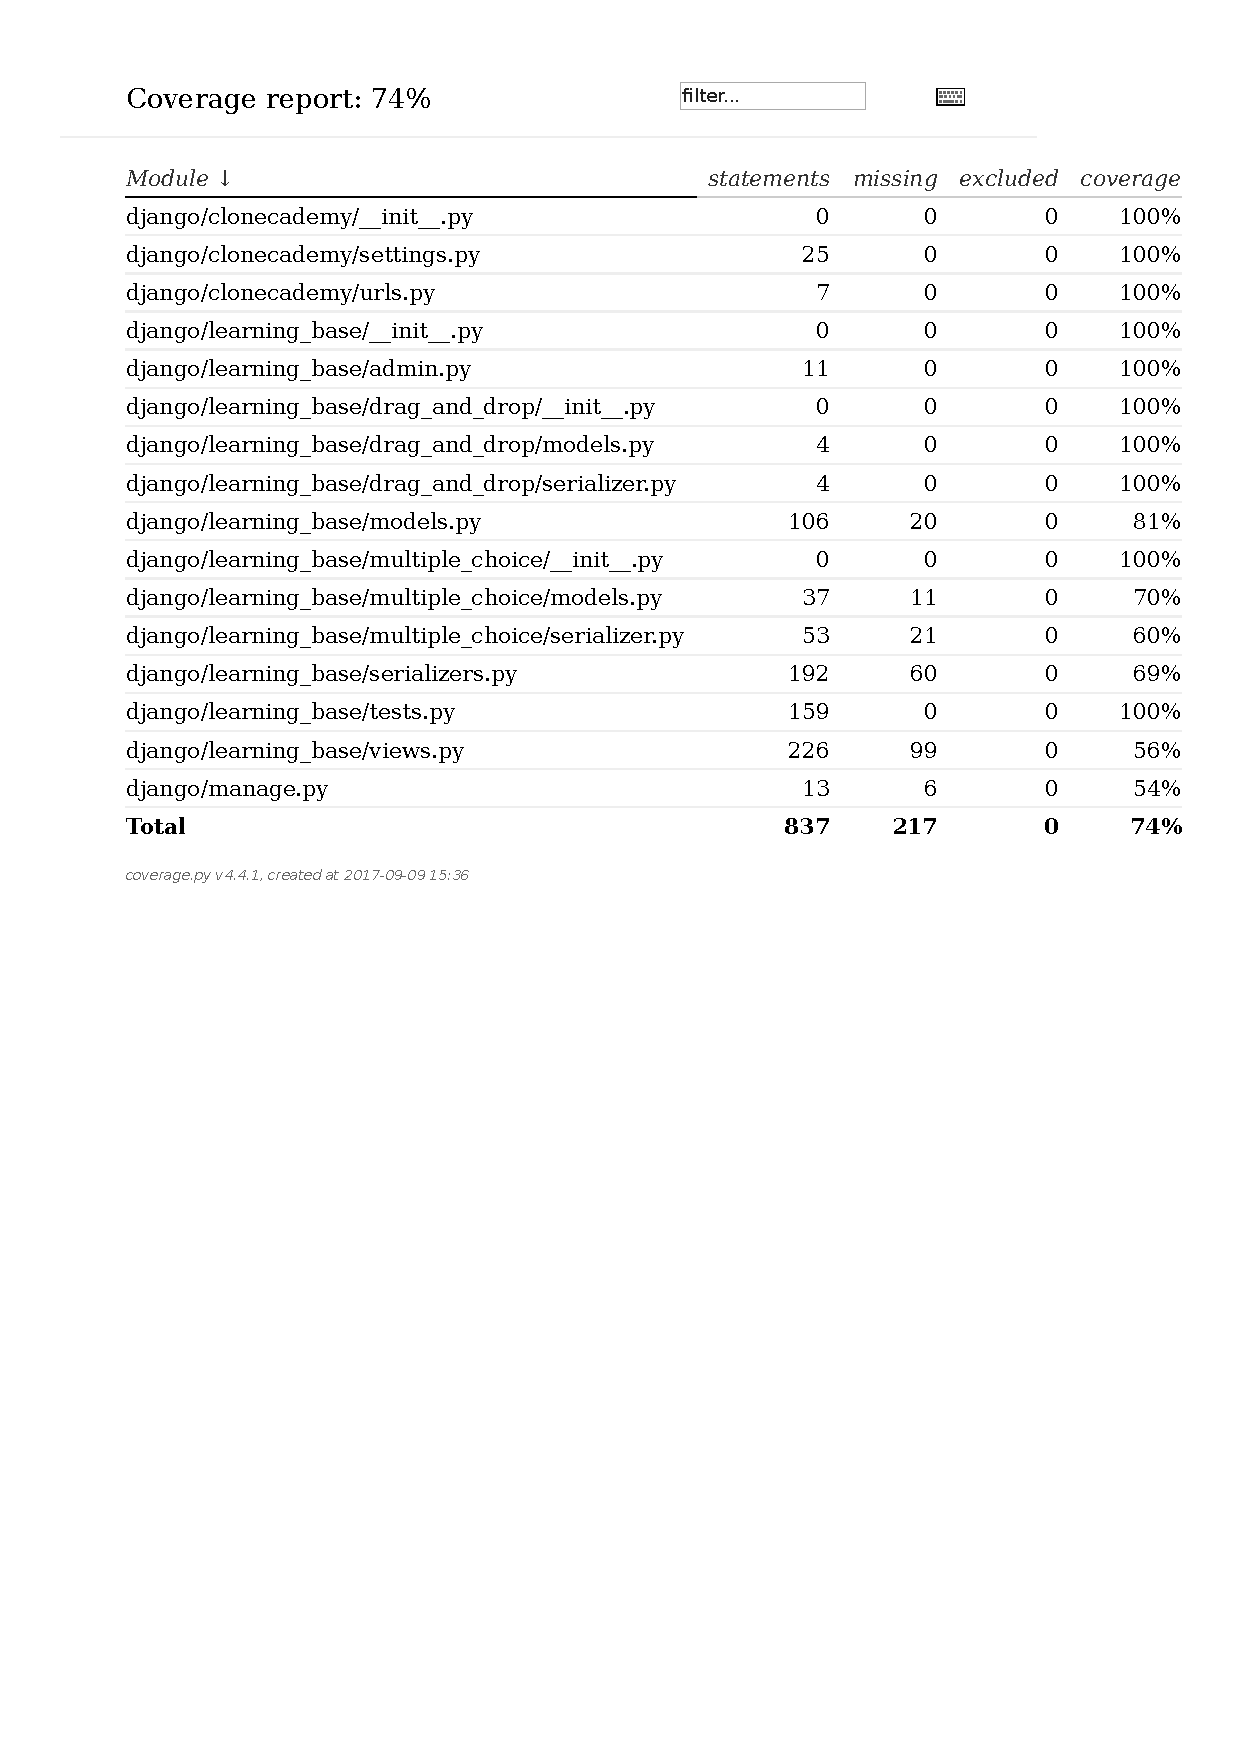
\includepdf[pages=-,pagecommand={},width=\textwidth]{appendix/coverage/django_test_07.pdf}
	
	\subsection{Security}
	\subsection*{bandit Output}
	\lstinputlisting{appendix/bandit/bandit_22f76.txt}
\section{Iteration 8 - 06.07.}
	Abgegebene Userstories: 12
	
	Commit Hash: cf525f64091e6c892b7e471fc8048bd8c056d69e
	
	
	\subsection{Checklisten}
	%\includepdf[pages=-,pagecommand={},width=\textwidth]{appendix/checklisten/12_01.pdf}

	\subsection{Veränderbarkeit}
	\subsubsection{ng lint Output}
	\lstinputlisting{appendix/ng_lint/ng_clean_8.txt}
	\subsection{pep8 Output}
	\lstinputlisting{appendix/pep8_07.txt}

	\subsection{Datensicherheit}
	\subsubsection{bandit Output}
	\lstinputlisting{appendix/bandit/bandit_cf525.txt}
\section{Iteration 9 - 13.07.}
	Abgegebene Userstories: keine
	
	Commit Hash: e2b7fed9dbc0e929bb28e7ccf30cd68aa0d73c19
	
	\subsection*{Checklisten}
	
	\subsection*{Veränderbarkeit}
	\subsubsection*{ng lint Output}
	\lstinputlisting{appendix/ng_lint/ng_clean_9.txt}
	\subsection*{pep8 Output}
	\lstinputlisting{appendix/pep8_07.txt}
	
	\subsection*{coverage Output}
	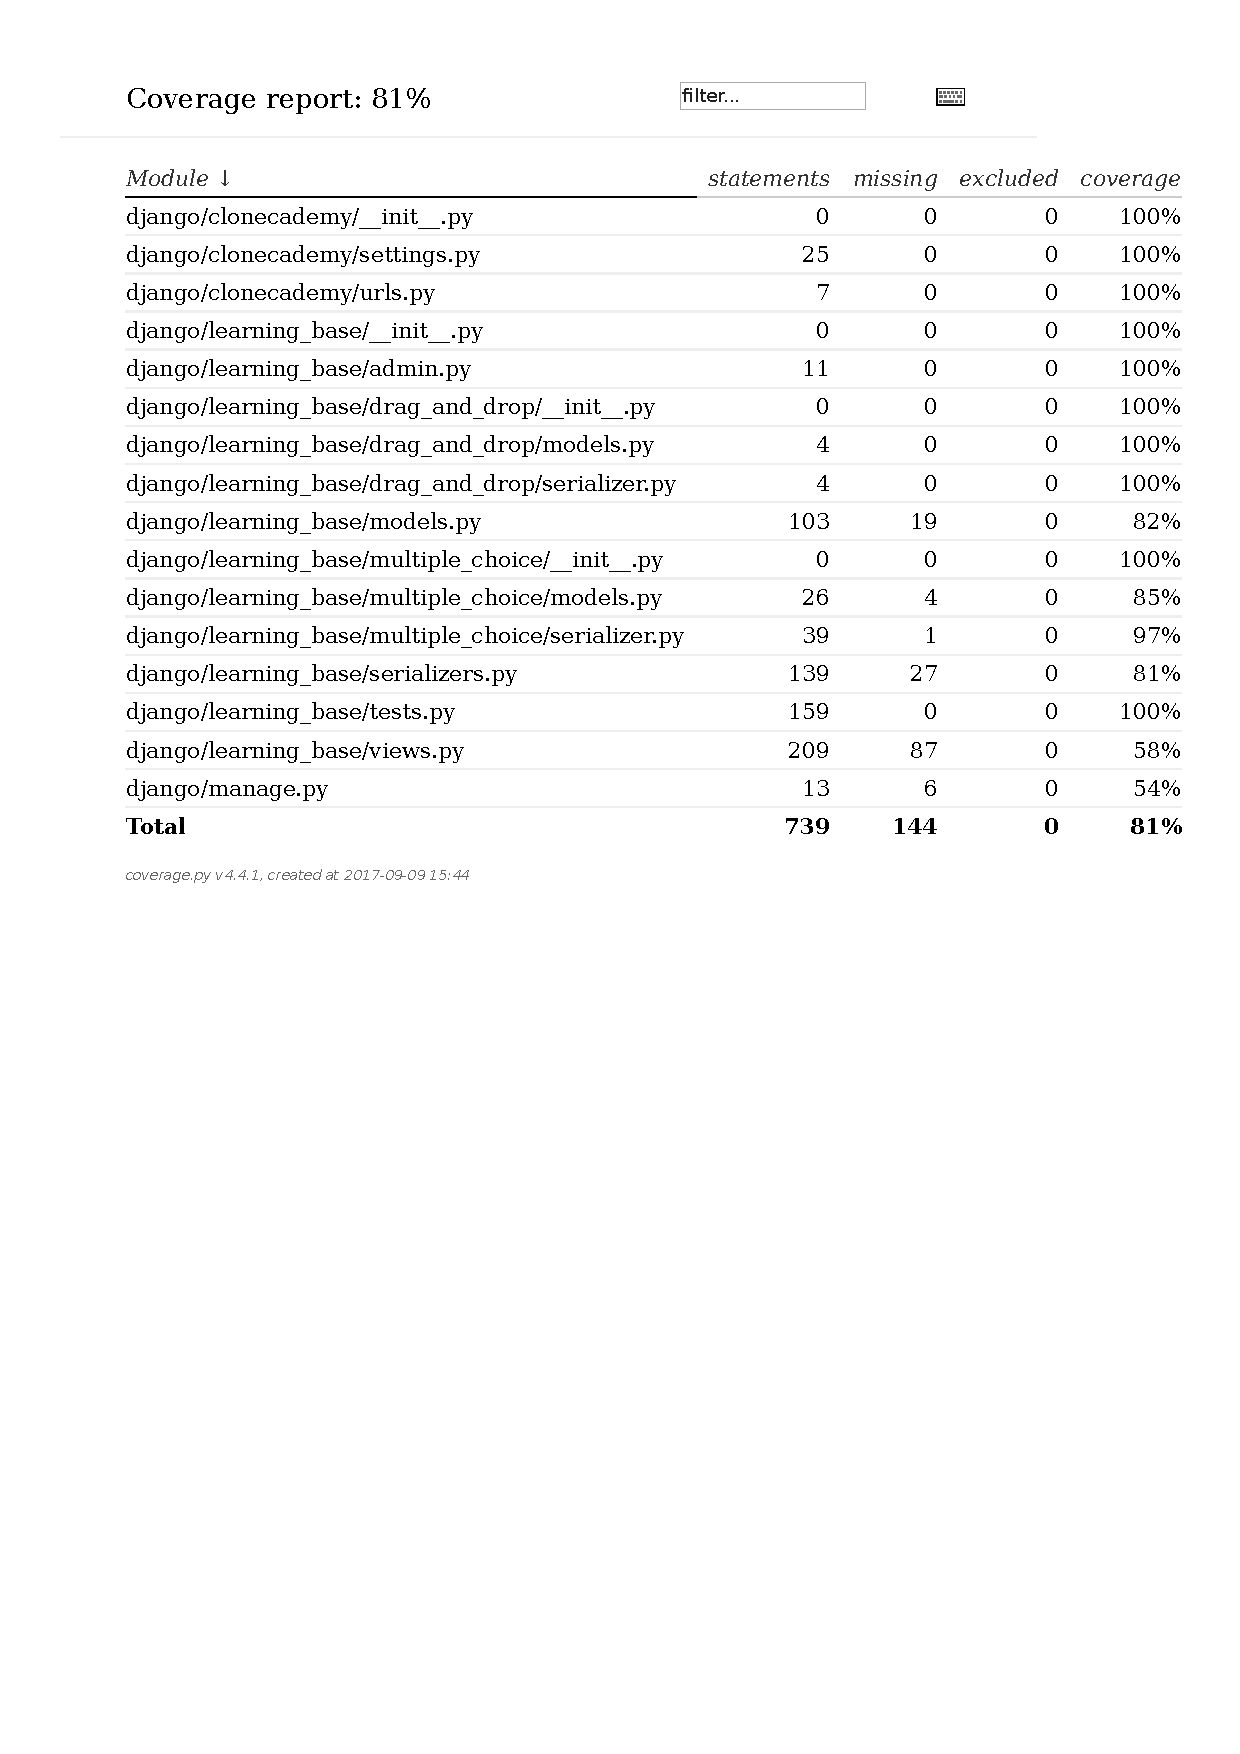
\includepdf[pages=-,pagecommand={},width=\textwidth]{appendix/coverage/django_test_09.pdf}
	
	\subsection*{Datensicherheit}

	
	\subsection*{bandit Output}
	\lstinputlisting{appendix/bandit/bandit_e2b7.txt}
	

% Abgabe QS Dokument war hier

\section{Iteration 10 - 20.07.}
	Ab Iteration 10 haben wir den gesamten QS-Prozess in seiner endgültigen Form durchgeführt.

	Abgegebene Userstories: 17, 18

	Commit Hash: f5845985bf7463a32f0f4f04279ea7481a32daaf
	
	\subsection*{Checklisten}
	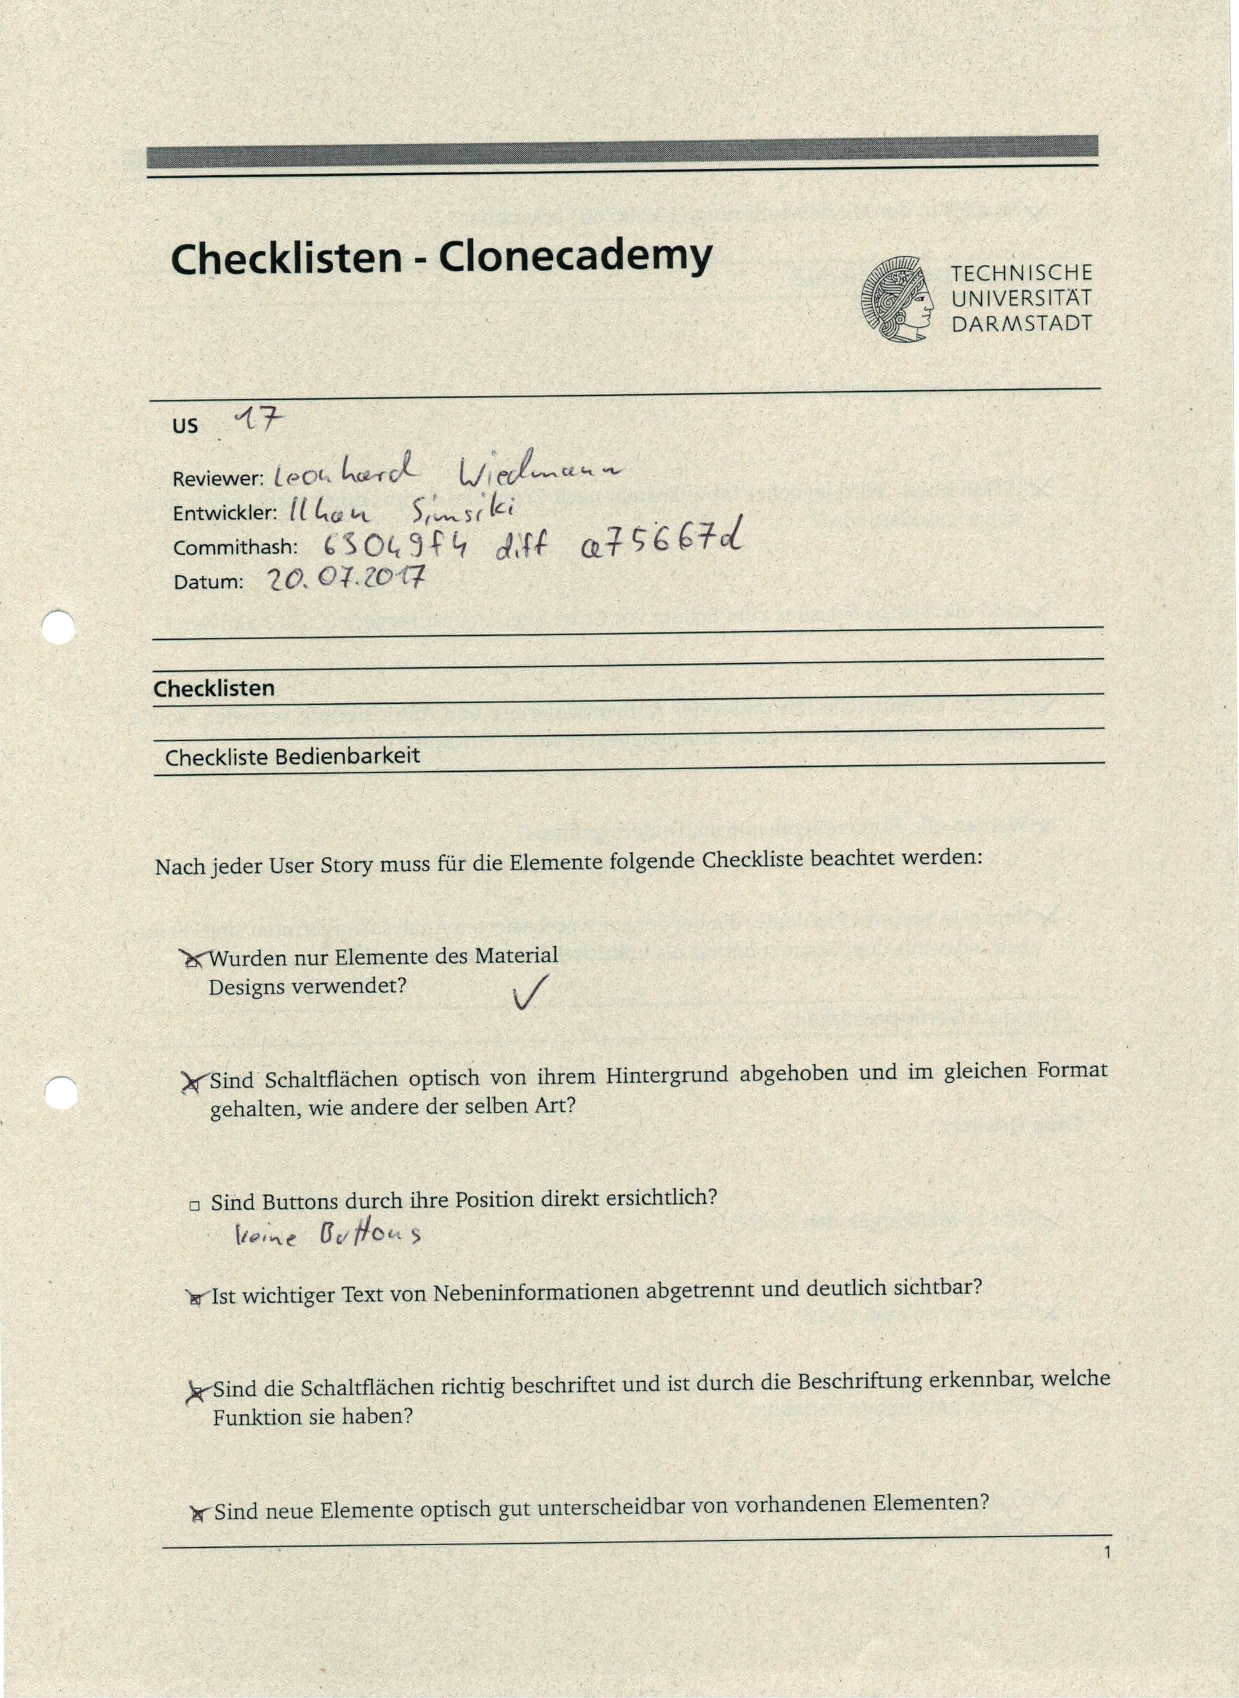
\includepdf[pages=-,pagecommand={},width=\textwidth]{appendix/checklisten/17_01.pdf}
	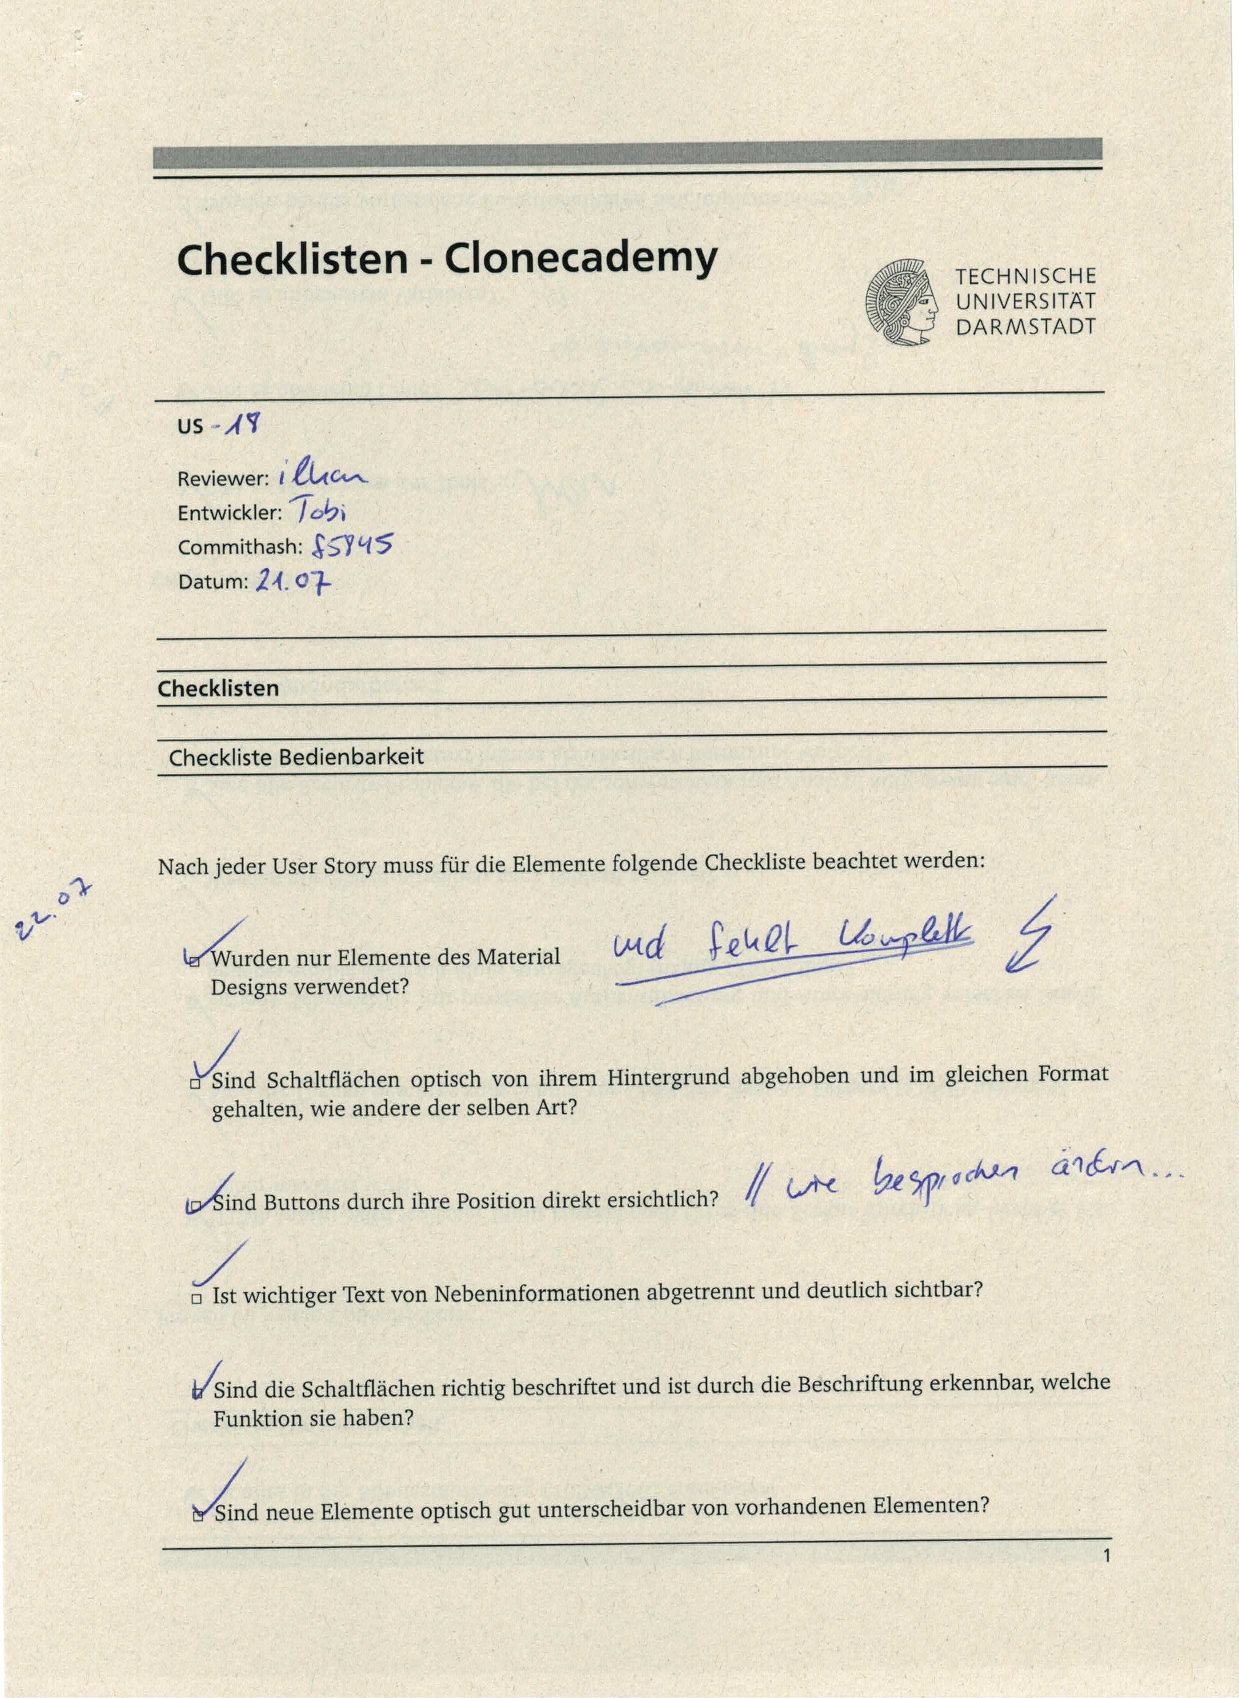
\includepdf[pages=-,pagecommand={},width=\textwidth]{appendix/checklisten/18_01.pdf}
	
	\subsection*{Veränderbarkeit}
	\subsubsection*{ng lint Output}
	\lstinputlisting{appendix/ng_lint/ng_clean_10.txt}
	
	\subsubsection*{pylint Output}
	\lstinputlisting{appendix/pylint/meldung_pylint_it10.txt}

	\subsubsection*{coverage Output}
	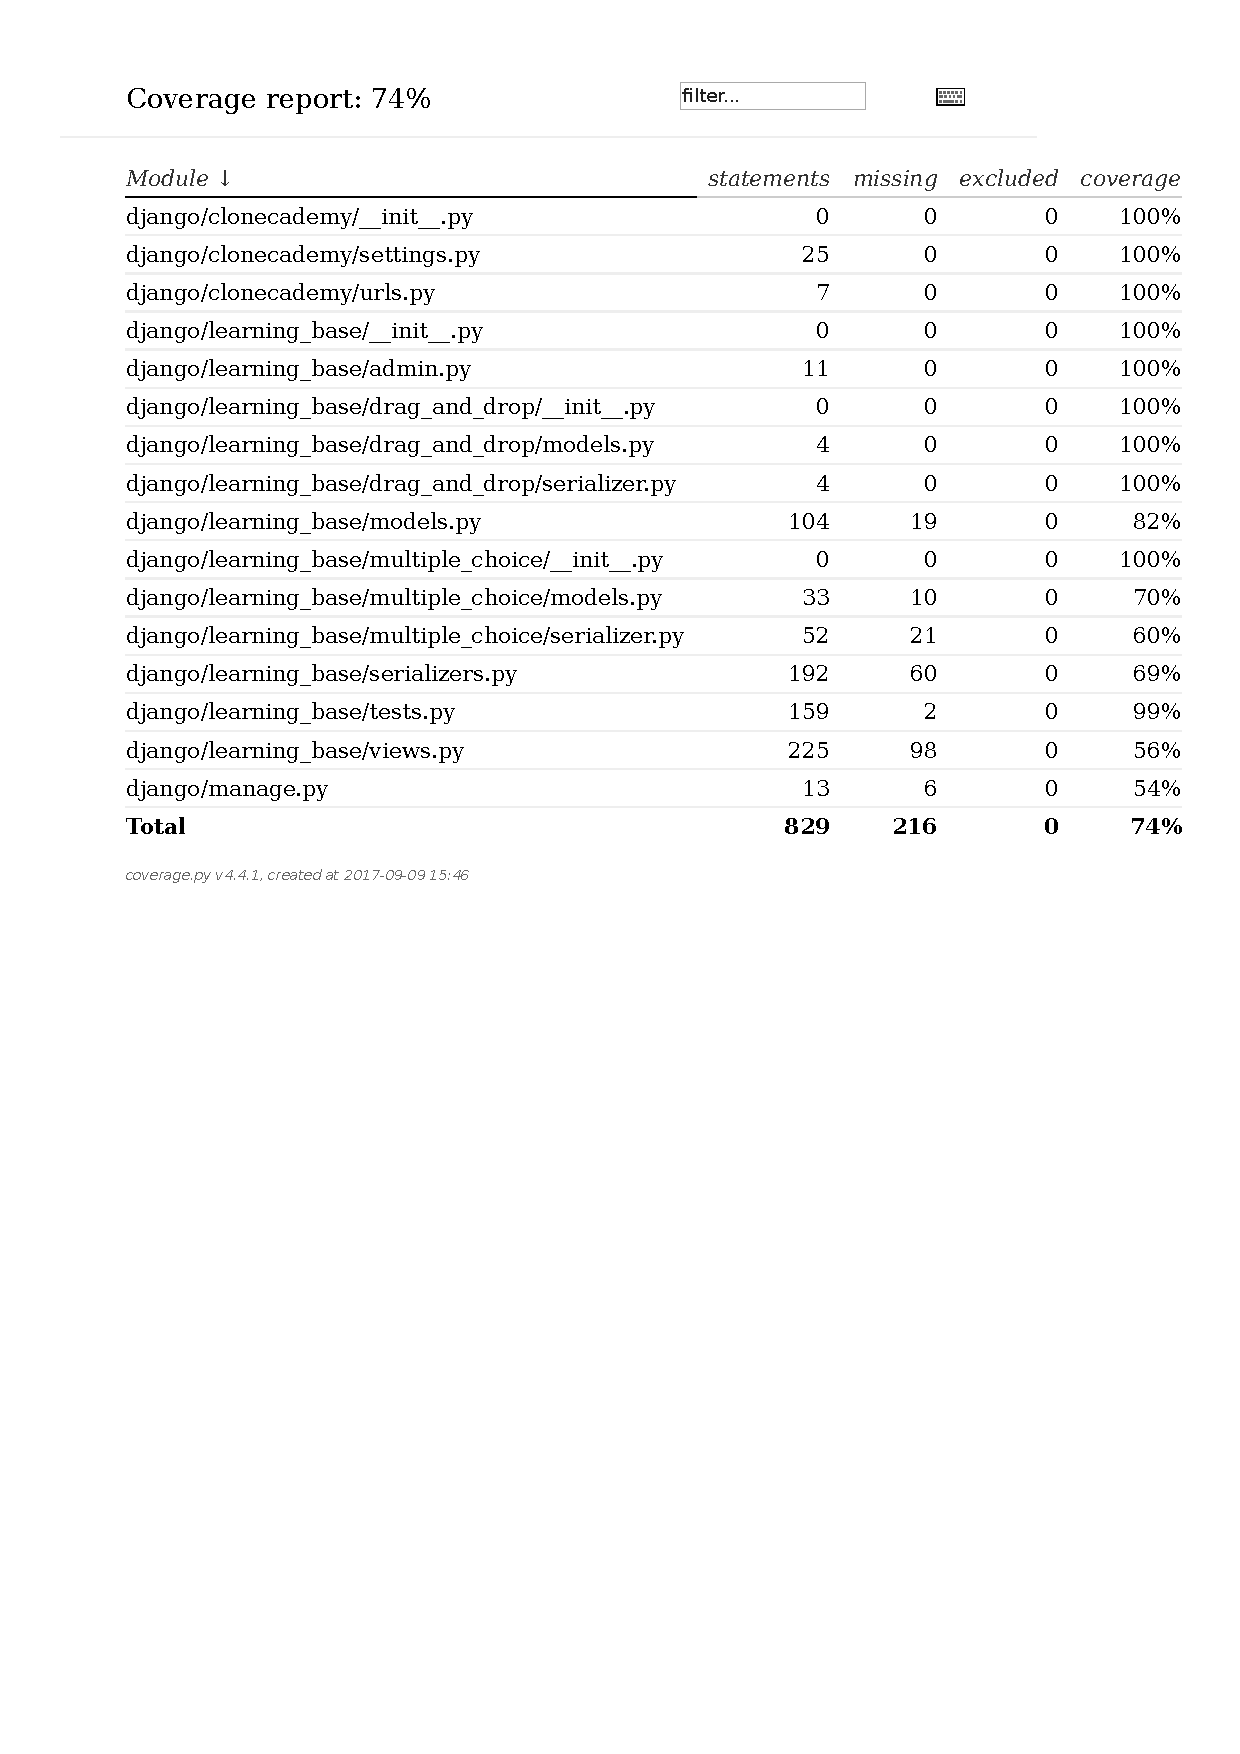
\includepdf[pages=-,pagecommand={},width=\textwidth]{appendix/coverage/django_test_10.pdf}

	\subsection*{Datensicherheit}
	\subsubsection*{bandit Output}
	\lstinputlisting{appendix/bandit/bandit_f584.txt}


	

\section{Iteration 11 - 27.07.}
	Abgegebene Userstories: 22
	
	Commit Hash: 2d17b38eecc8bbd754534a564ff2a22d60ee5f71
	
	\subsection*{Checklisten}
	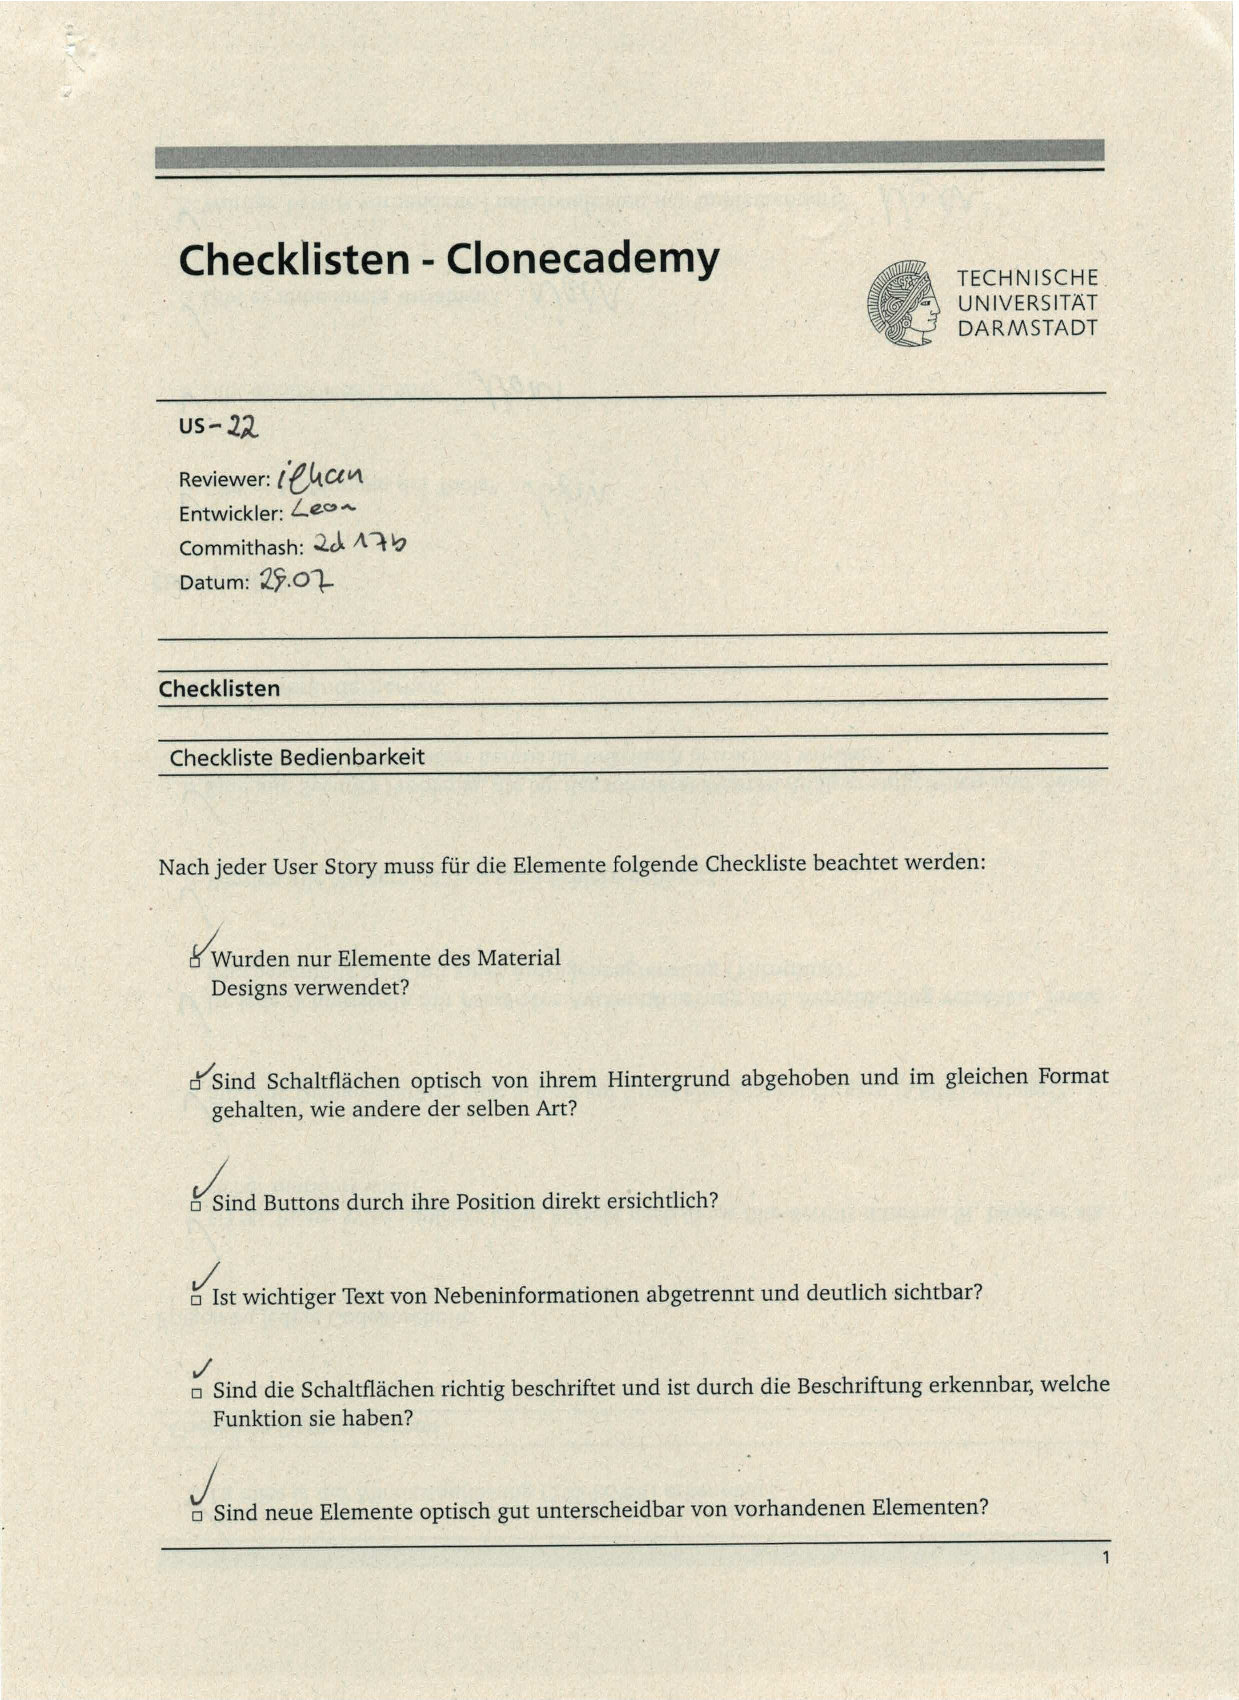
\includepdf[pages=-,pagecommand={},width=\textwidth]{appendix/checklisten/22_01.pdf}
	
	\subsection*{Veränderbarkeit}
	\subsubsection*{ng lint Output}
	\lstinputlisting{appendix/ng_lint/ng_clean_11.txt}
	
	\subsubsection*{pylint Output}
	\lstinputlisting{appendix/pylint/meldung_pylint_it11.txt}

	\subsubsection*{coverage Output}
	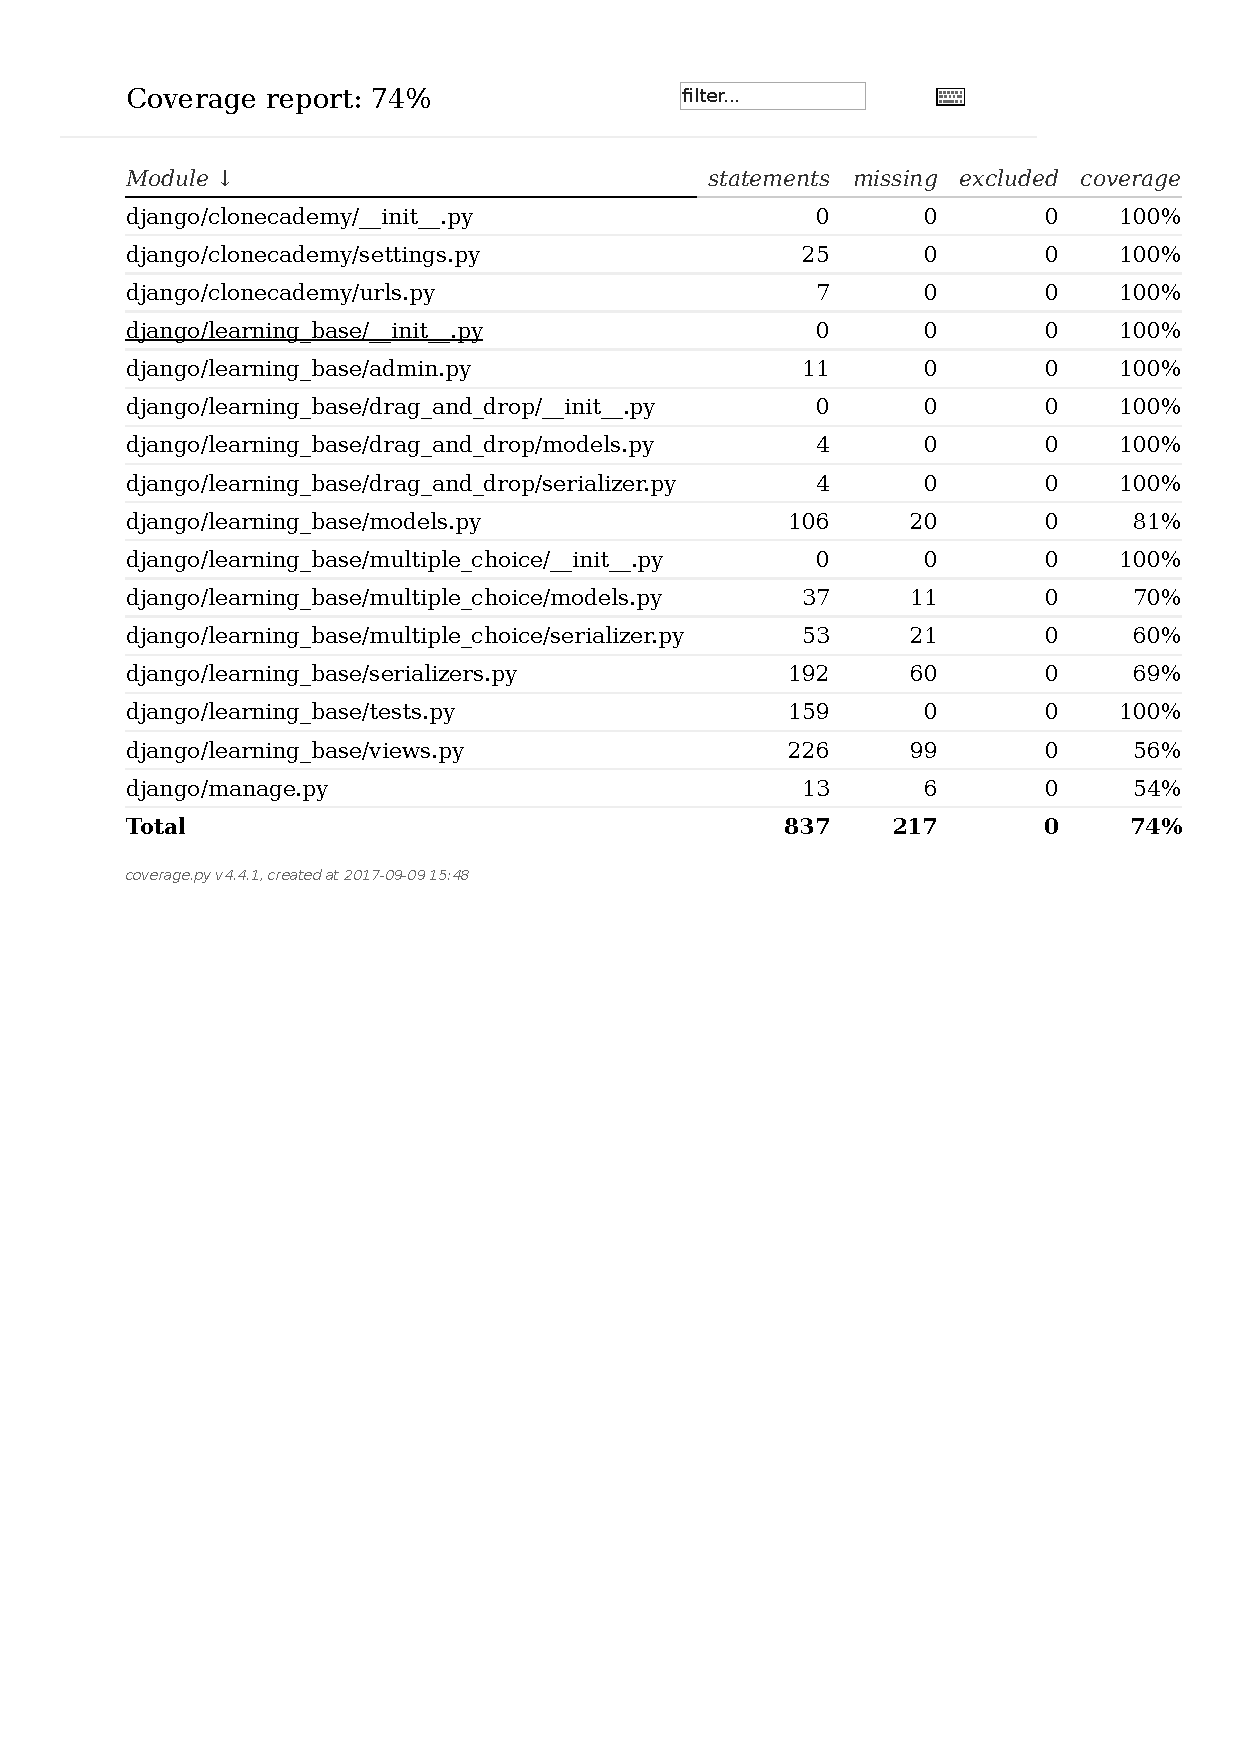
\includepdf[pages=-,pagecommand={},width=\textwidth]{appendix/coverage/django_test_11.pdf}
	
	\subsection*{Datensicherheit}
	\subsubsection*{bandit Output}
	\lstinputlisting{appendix/bandit/bandit_2d17b.txt}


	
\section{Iteration 12 - 03.08.}
	Abgegebene Userstories: 4,19,20
	
	Commit Hash: 7af0e8284c862f9841d8101c6f4569adb0c6289c
	
	\subsection{Checklisten}
	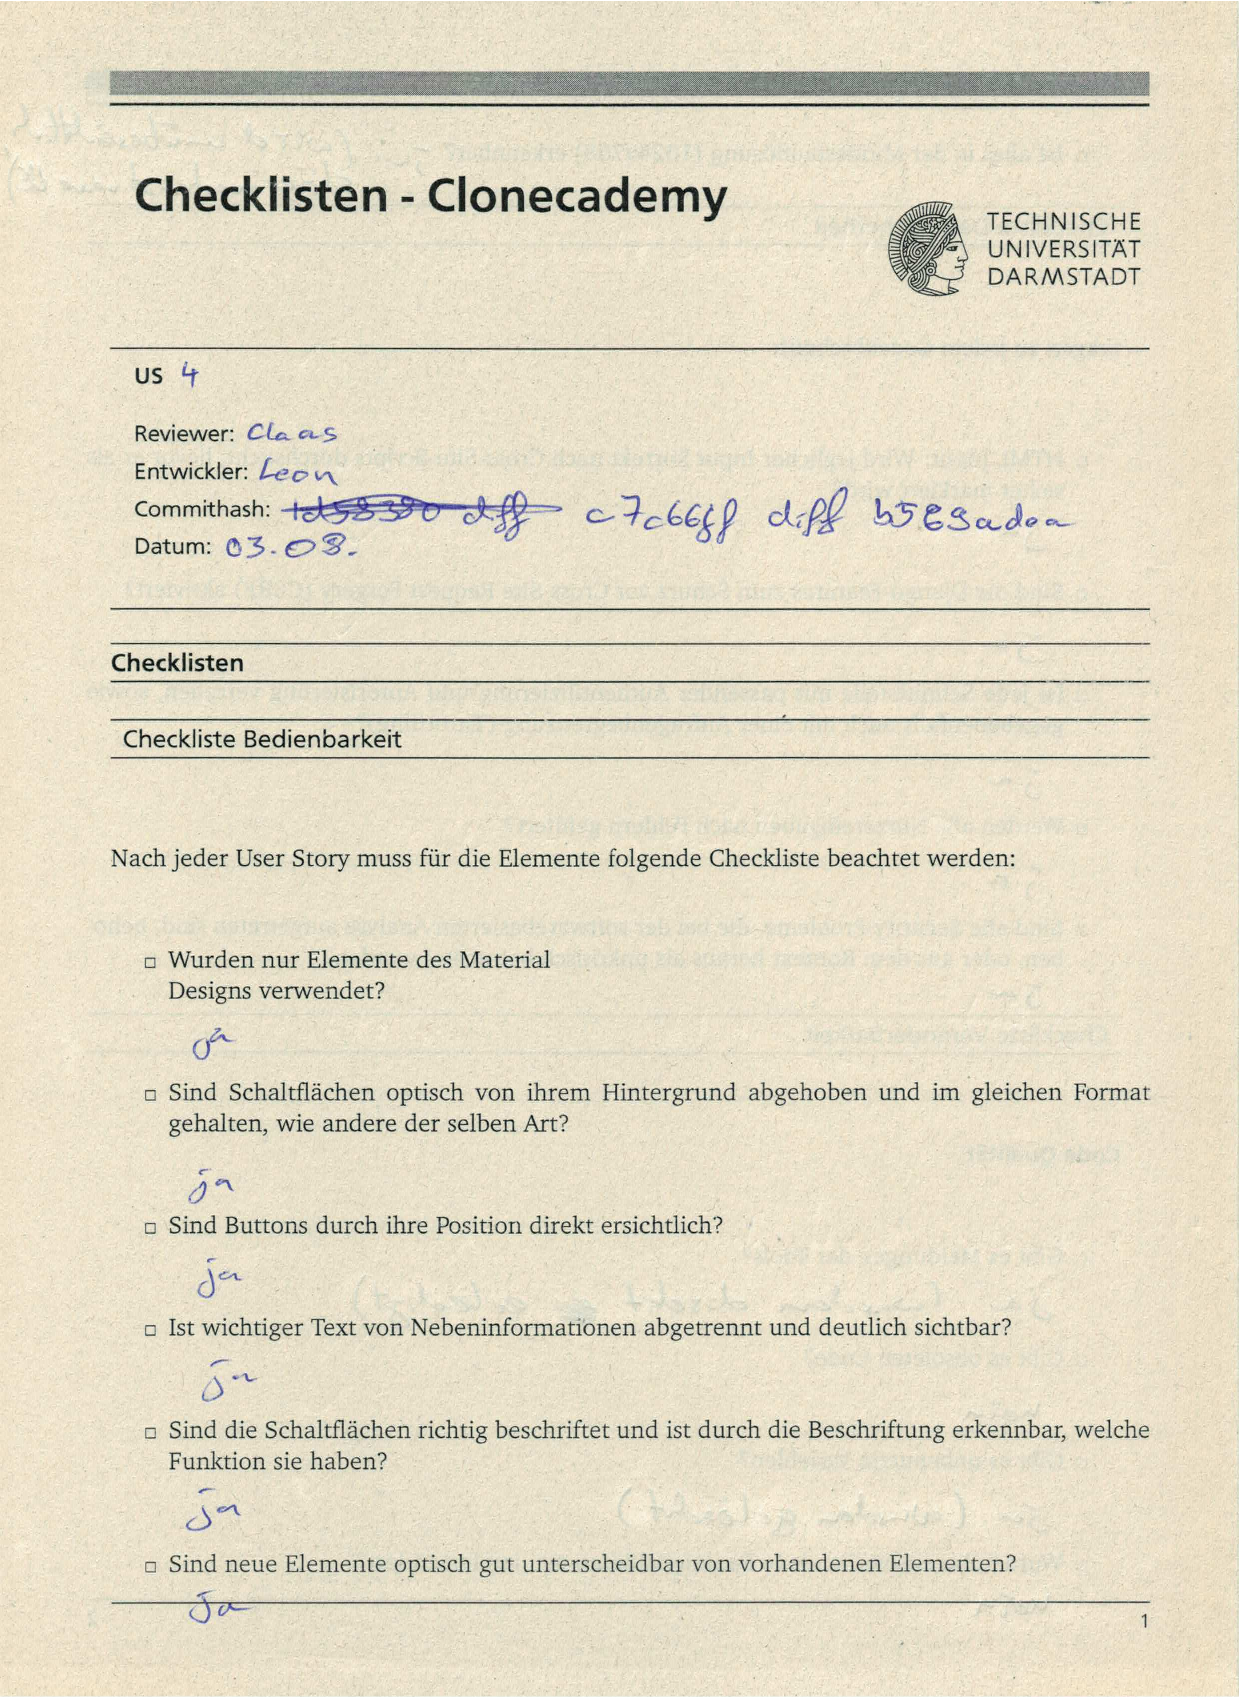
\includepdf[pages=-,pagecommand={},width=\textwidth]{appendix/checklisten/04_01.pdf}
	%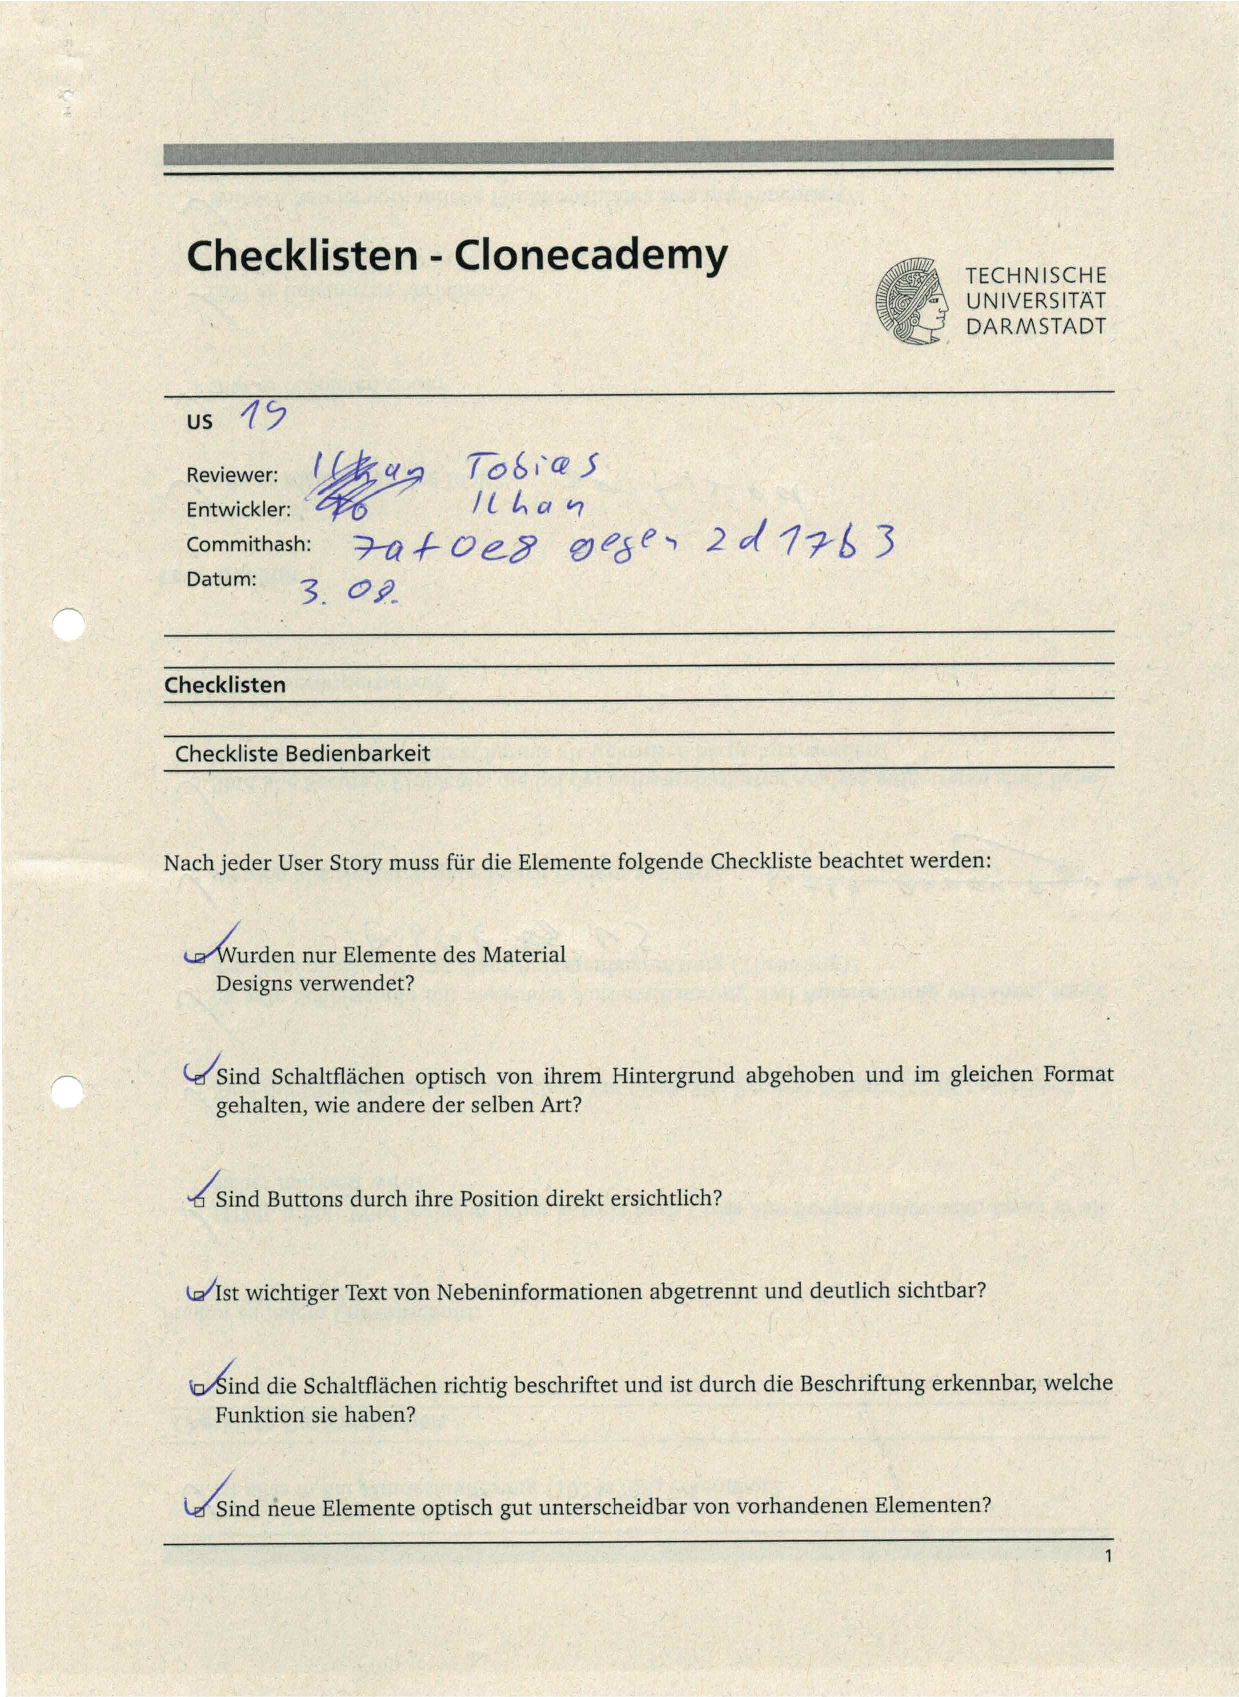
\includepdf[pages=-,pagecommand={},width=\textwidth]{appendix/checklisten/19_01.pdf}
	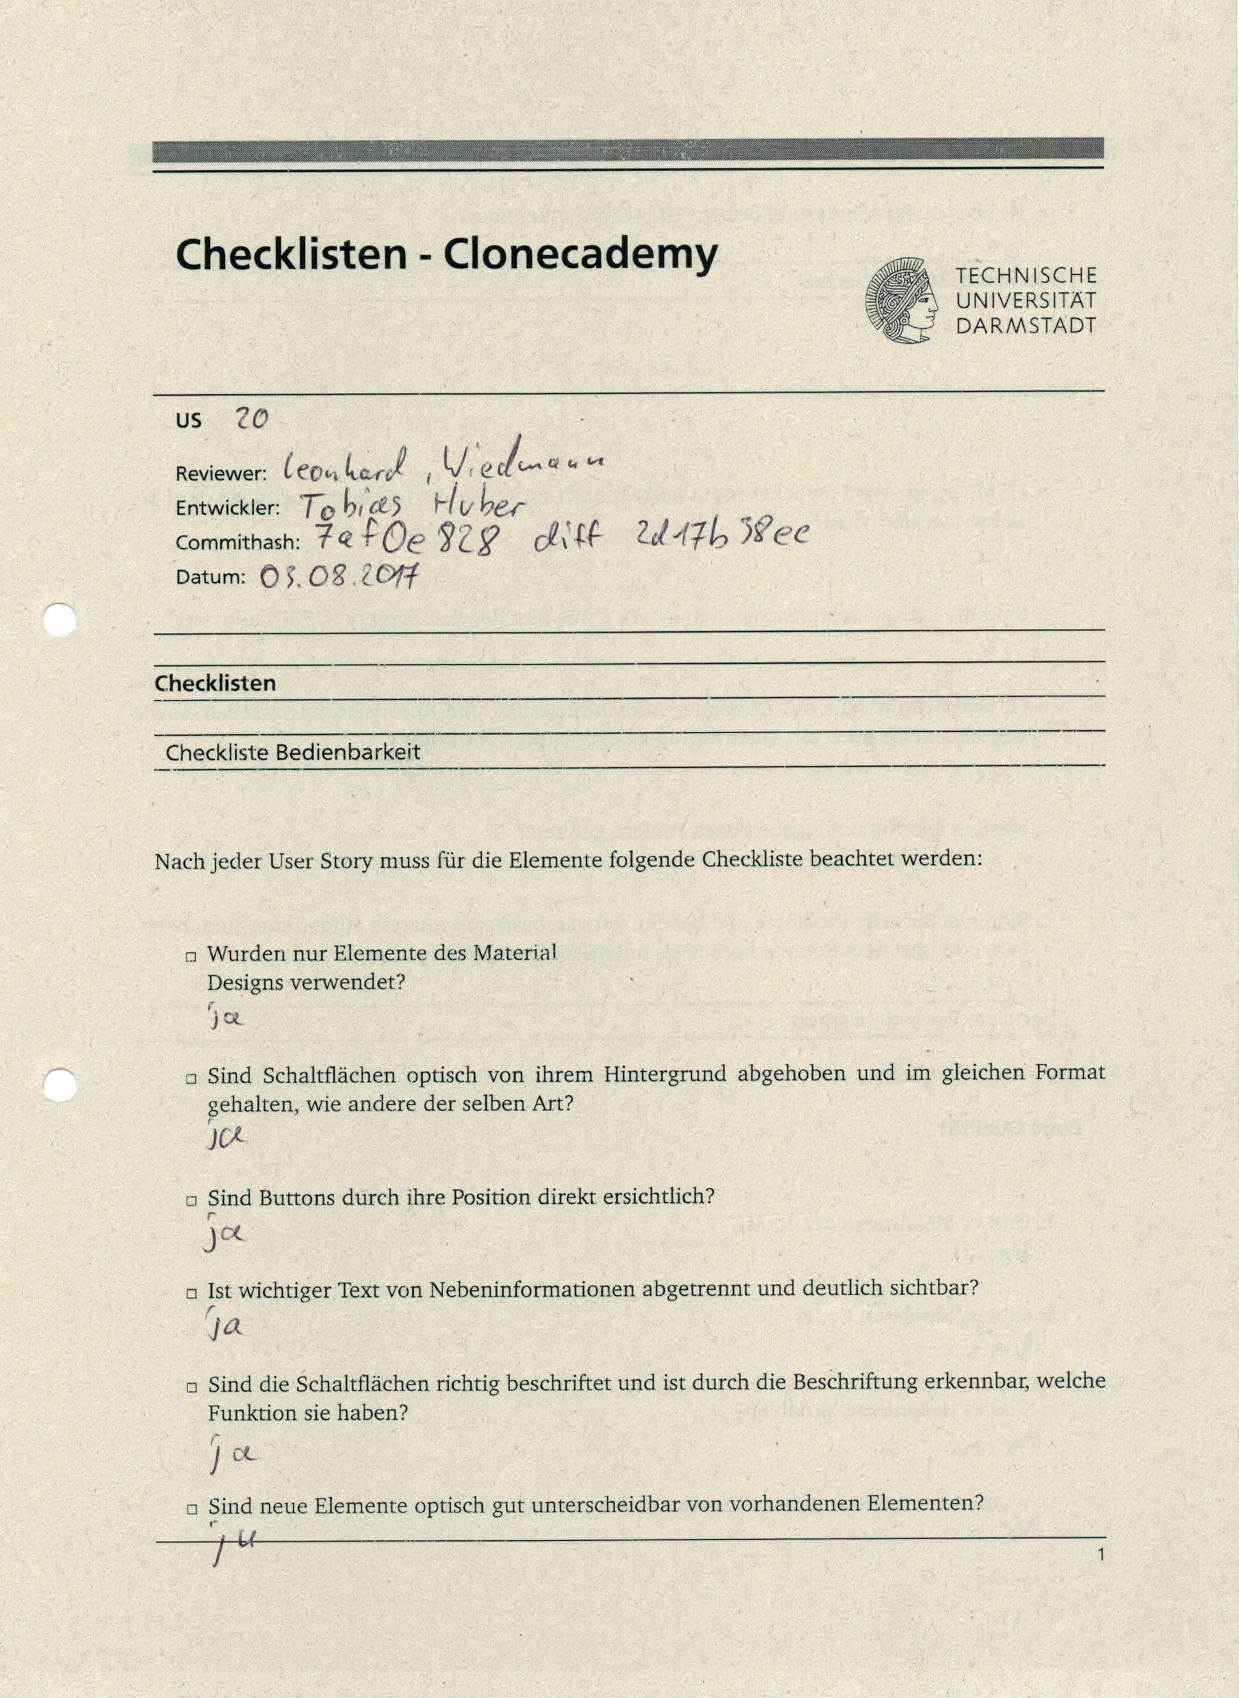
\includepdf[pages=-,pagecommand={},width=\textwidth]{appendix/checklisten/20_01.pdf}
	
	\subsection{Veränderbarkeit}
	\subsubsection{ng lint Output}
	\lstinputlisting{appendix/ng_lint/ng_clean_12.txt}
	
	\subsubsection{pylint Output}
	\lstinputlisting{appendix/pylint/meldung_pylint_it12.txt}

	\subsubsection{coverage Output}
	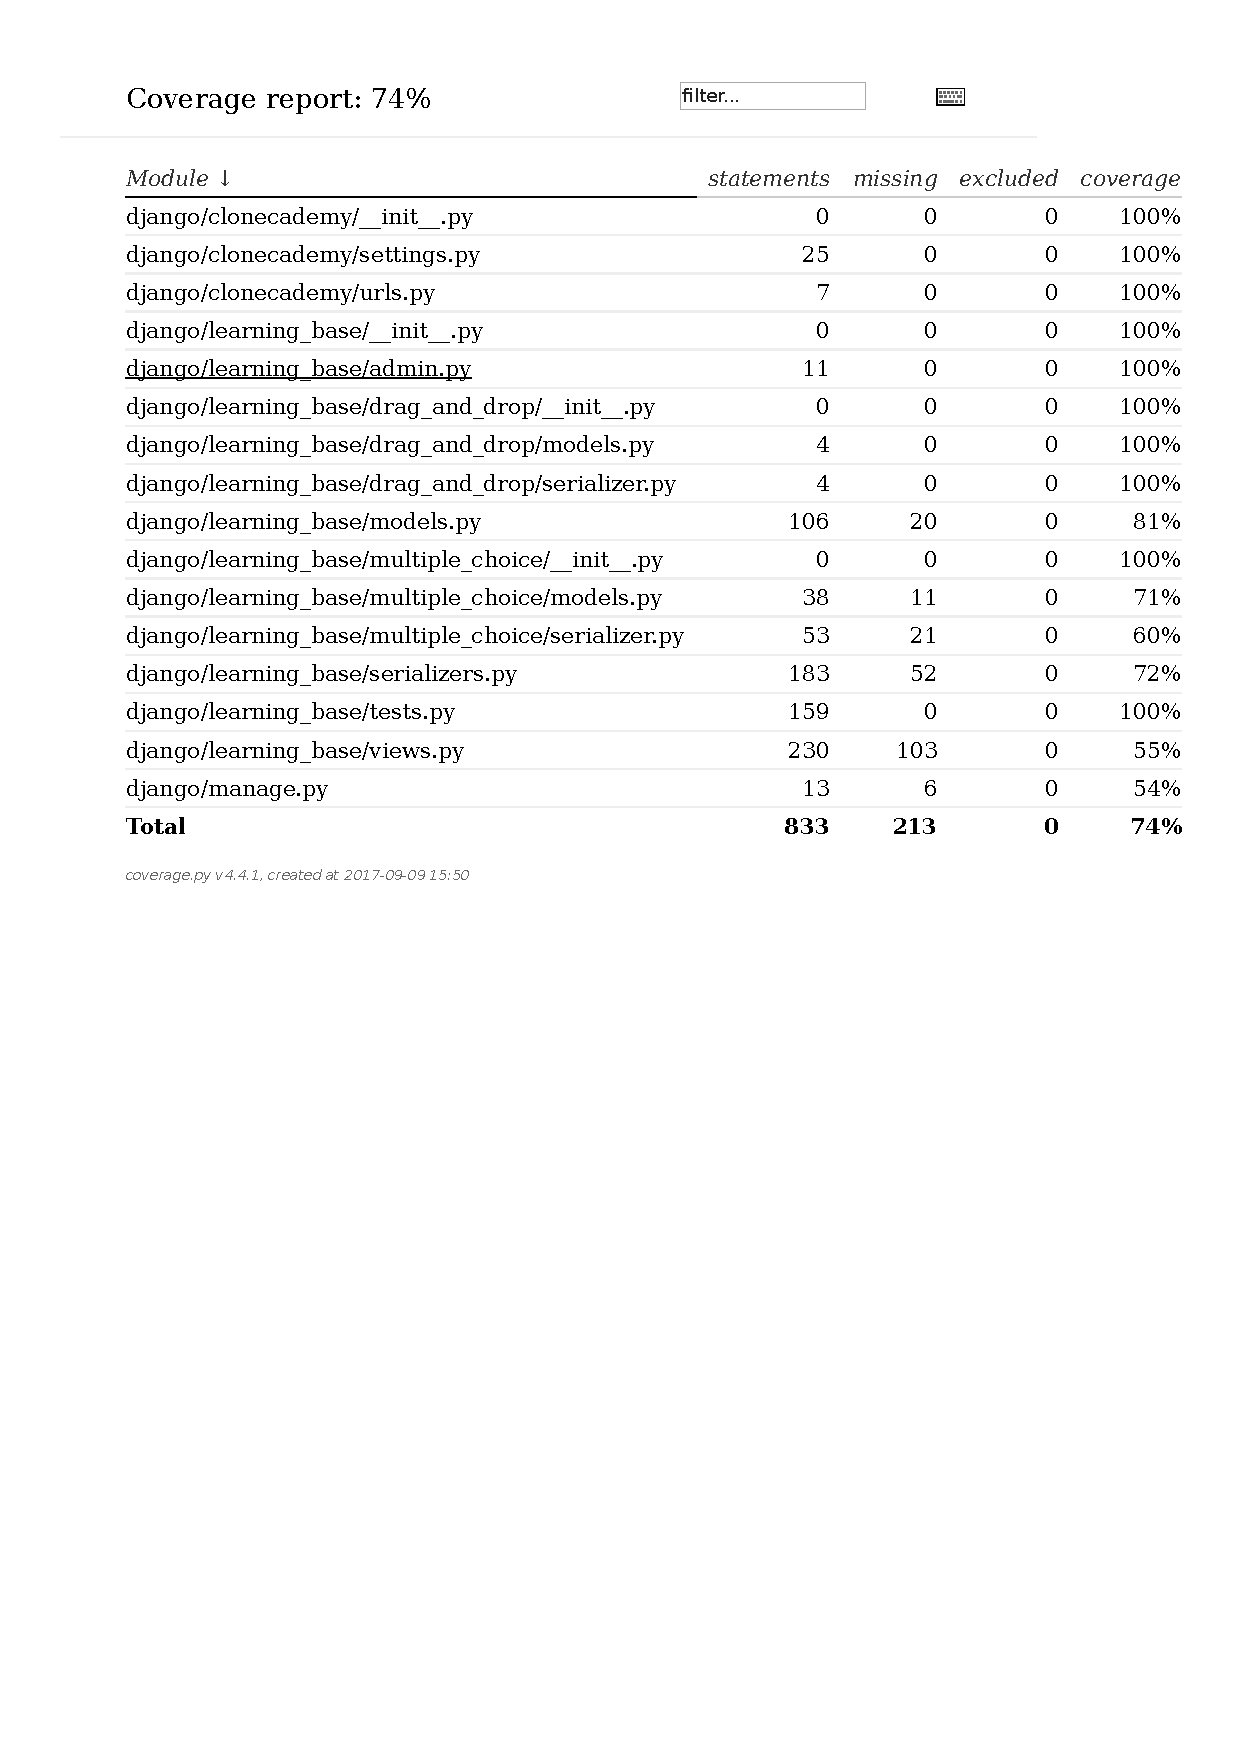
\includepdf[pages=-,pagecommand={},width=\textwidth]{appendix/coverage/django_test_12.pdf}

	\subsection{Datensicherheit}
	\subsubsection{bandit Output}
	\lstinputlisting{appendix/bandit/bandit_7af0e.txt}
	

\section*{Iteration 13 - 10.08.}
	Abgegebene Userstories: 24, 26, 28

	Commit Hash: b5e9a319bf3bd0bc33e544ff615e1bd8b62c7931
	
	\subsection{Checklisten}
	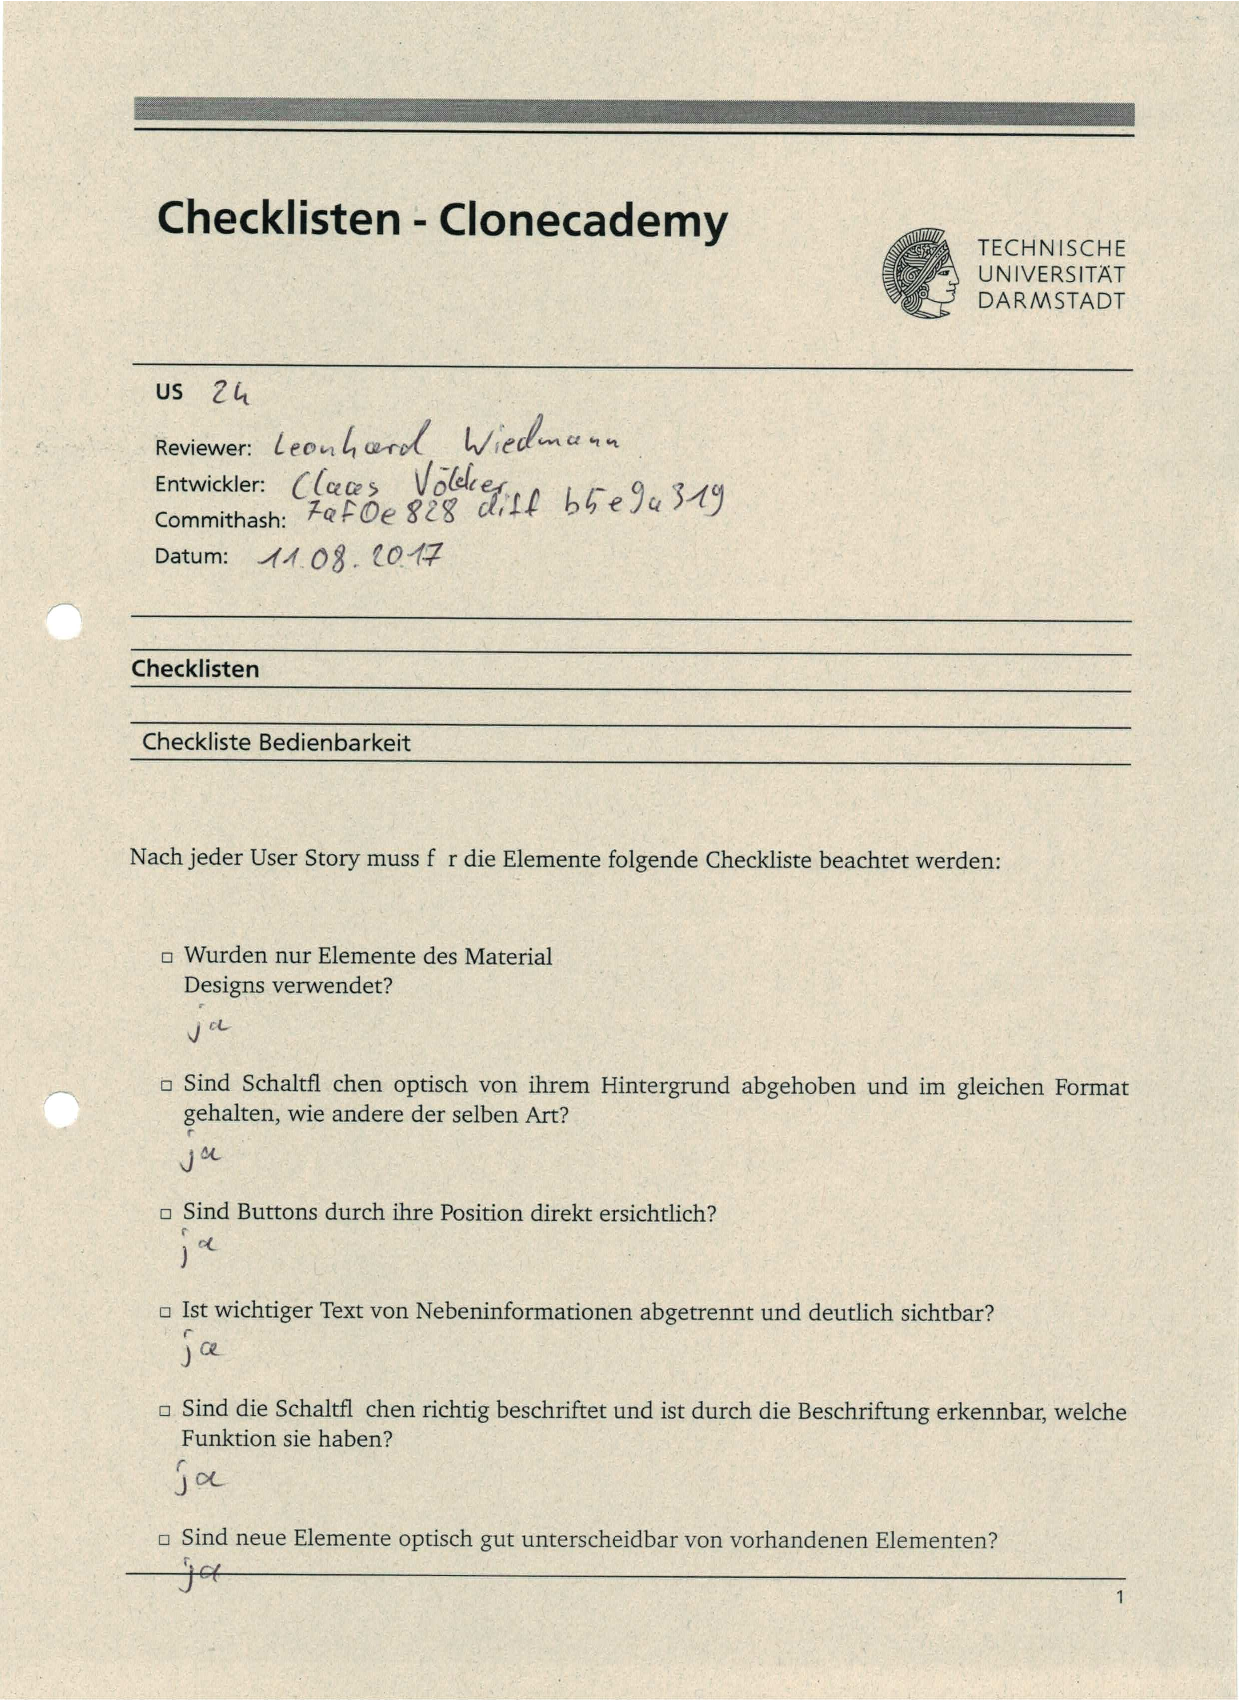
\includepdf[pages=-,pagecommand={},width=\textwidth]{appendix/checklisten/24_01.pdf}
	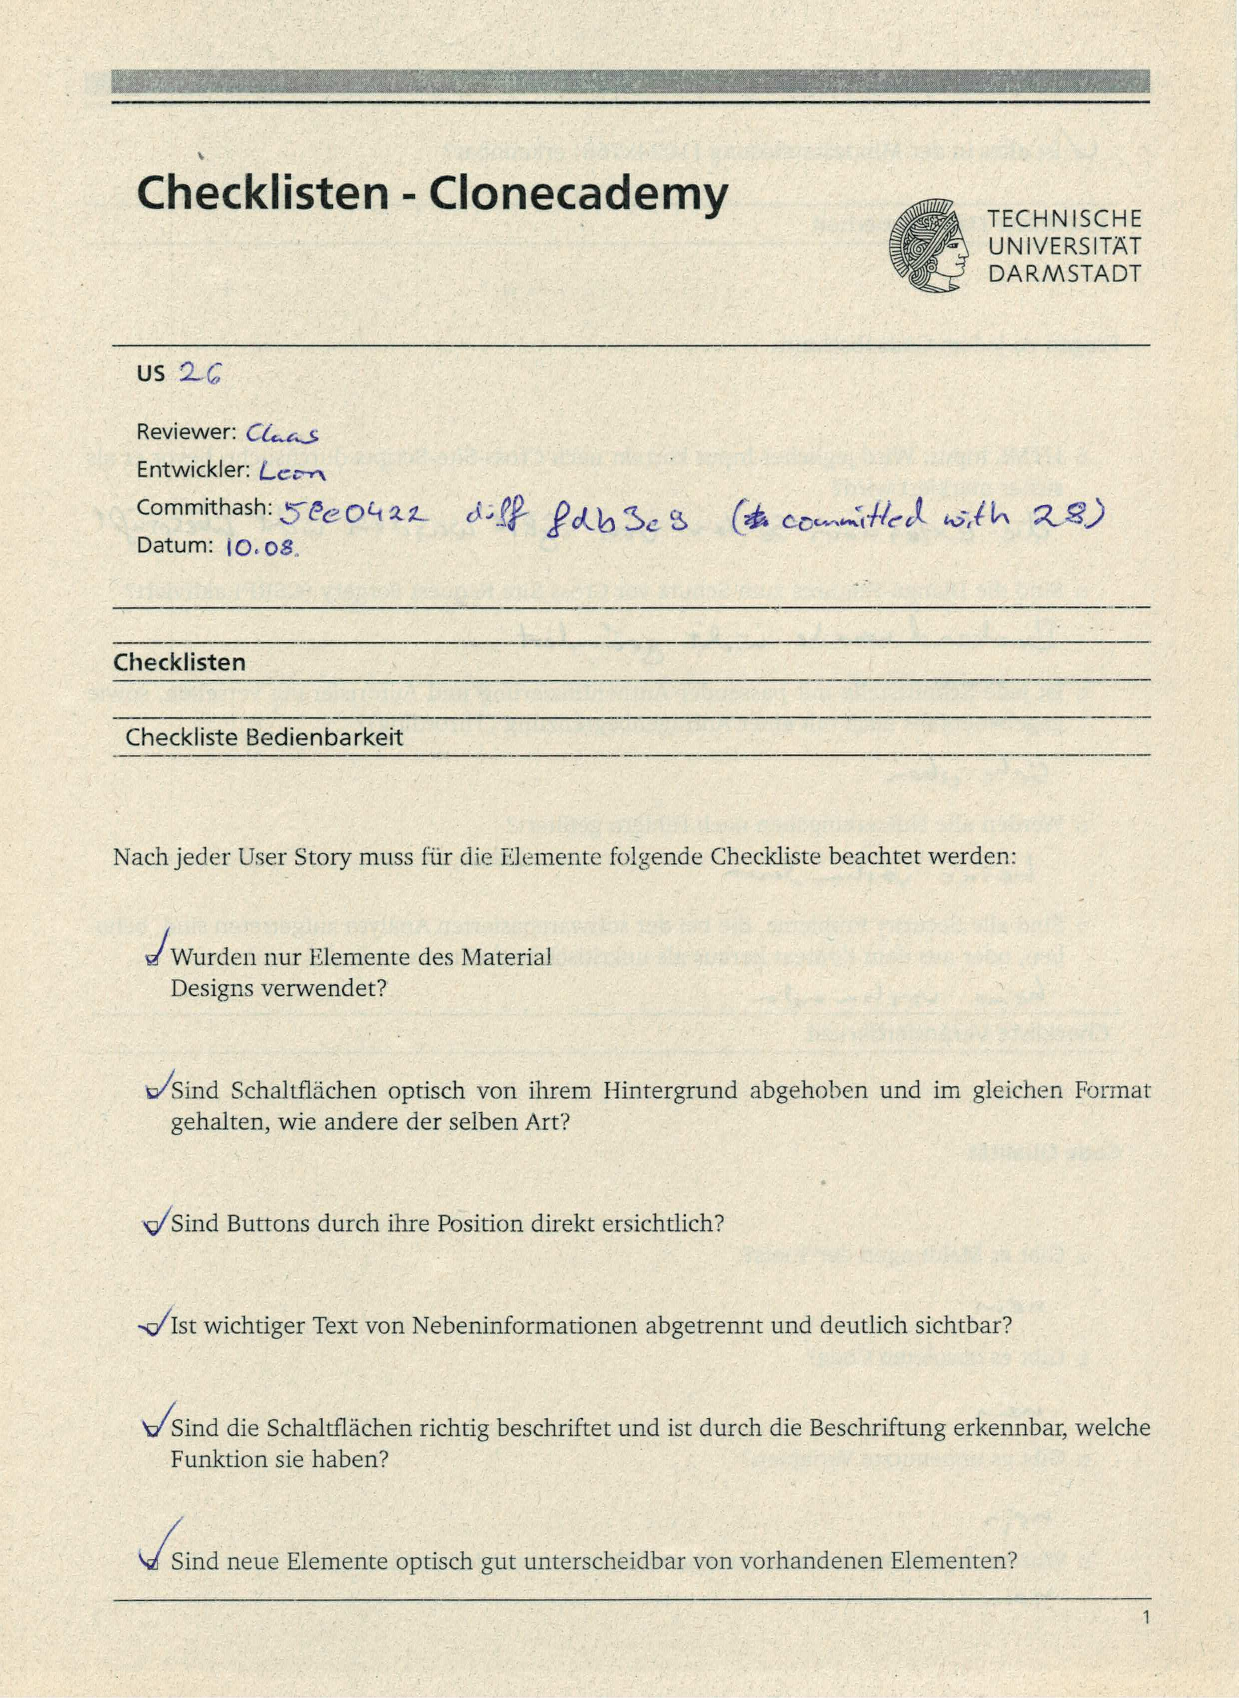
\includepdf[pages=-,pagecommand={},width=\textwidth]{appendix/checklisten/26_01.pdf}
	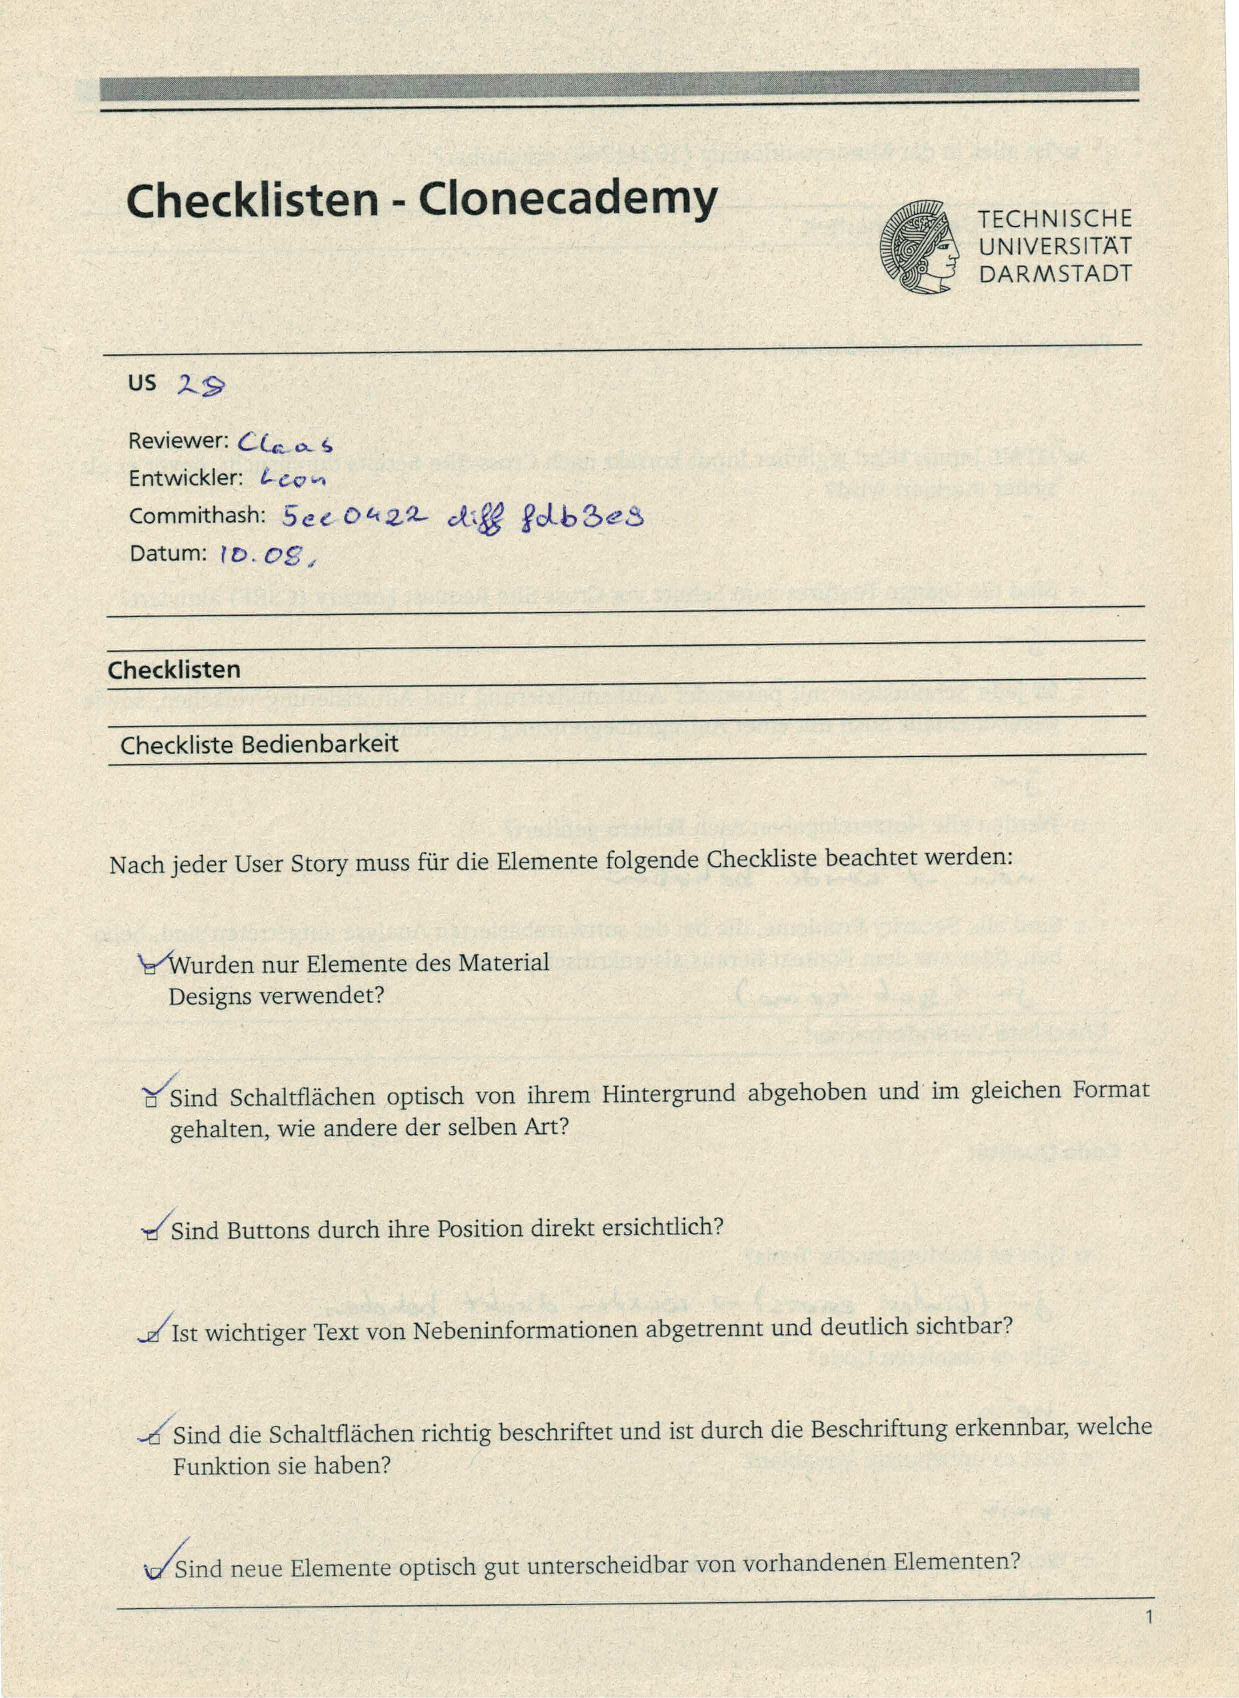
\includepdf[pages=-,pagecommand={},width=\textwidth]{appendix/checklisten/28_01.pdf}

	\subsection*{Veränderbarkeit}
	\subsubsection*{ng lint Output}
	\lstinputlisting{appendix/ng_lint/ng_clean_13.txt}

	\subsubsection*{pylint Output}
	\lstinputlisting{appendix/pylint/meldung_pylint_it13.txt}

	\subsubsection*{coverage Output}
	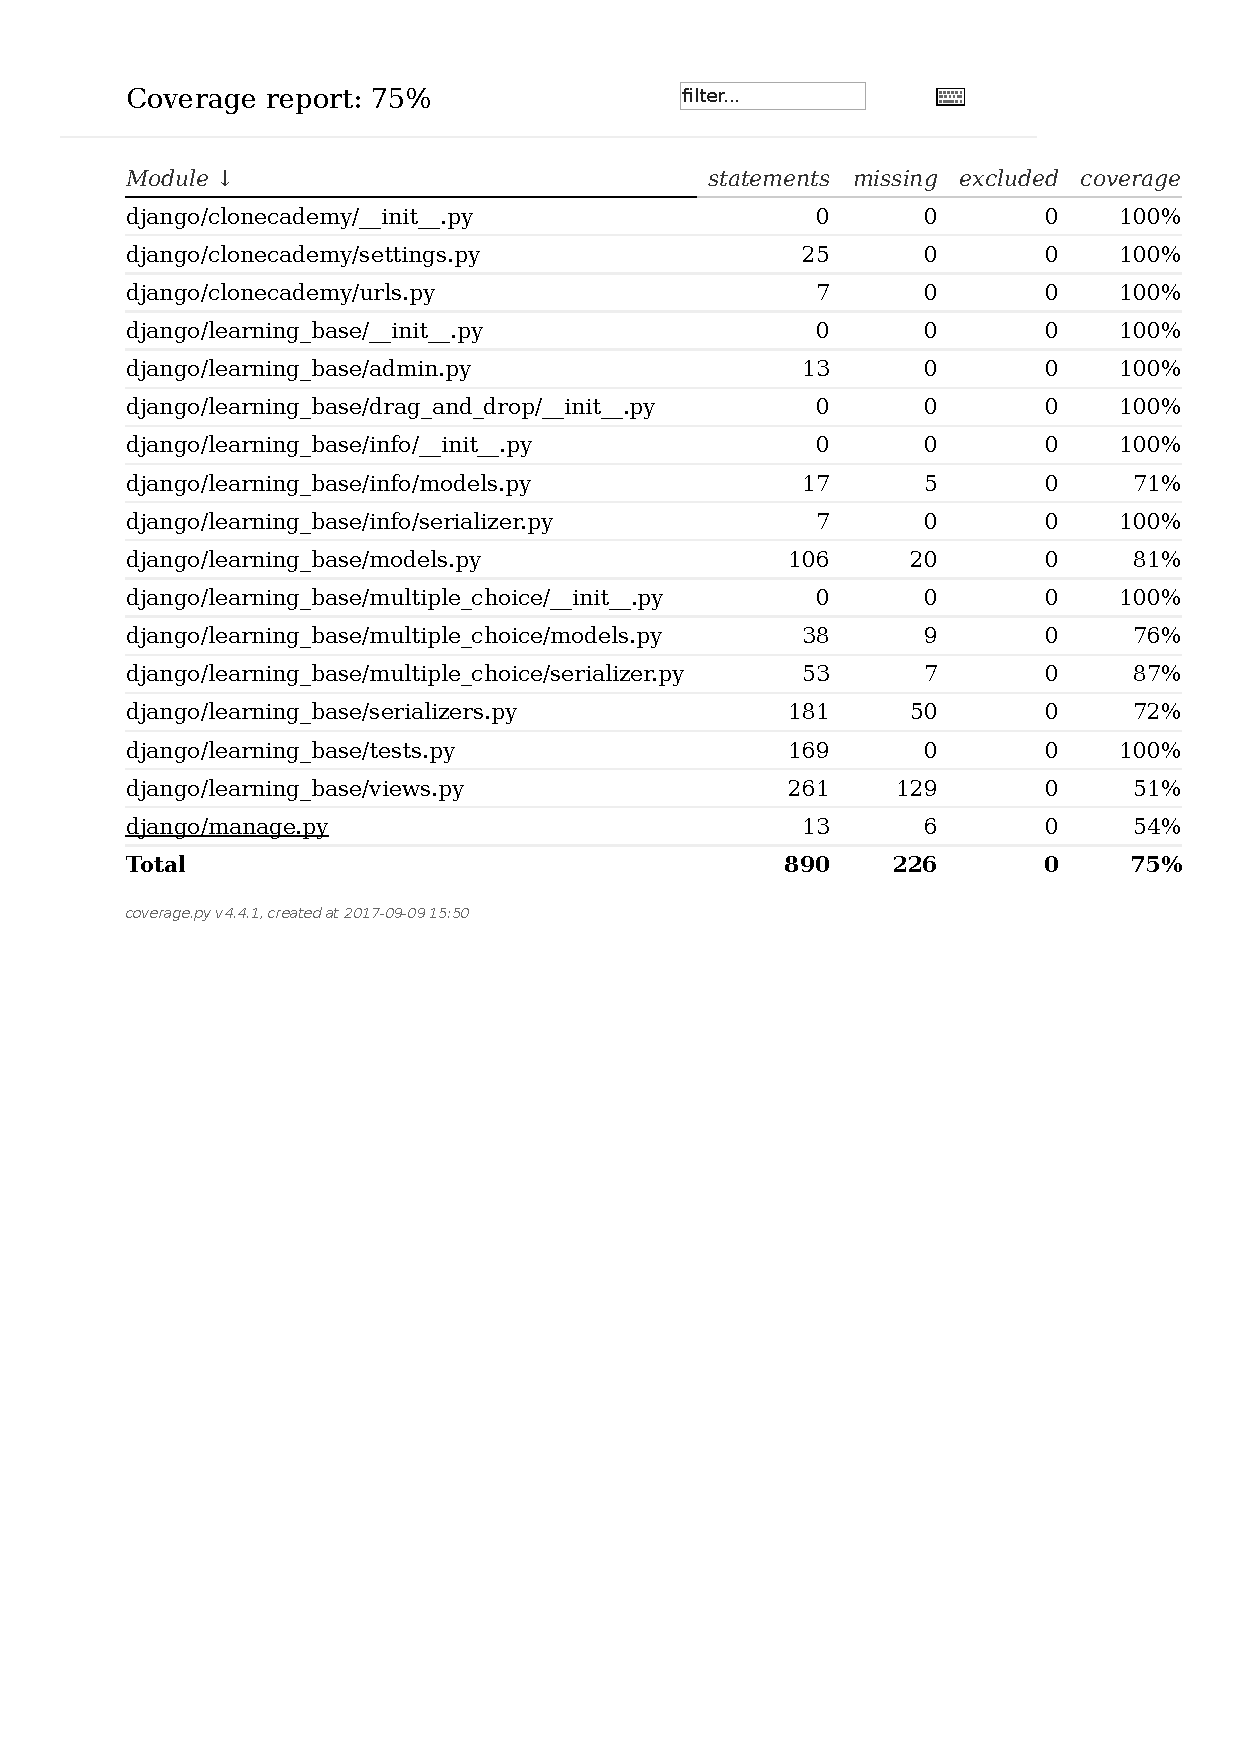
\includepdf[pages=-,pagecommand={},width=\textwidth]{appendix/coverage/django_test_13.pdf}

	\subsection*{Datensicherheit}
	\subsubsection*{bandit Output}
	\lstinputlisting{appendix/bandit/bandit_b5e9a.txt}
	

\section{Iteration 14 - 17.08.}
	Abgegebene Userstories: 25,27
	
	Commit Hash: ba0fab4c21d736b0f67f8fe21ef90c0da810ac4b
	
	\subsection{Checklisten}
	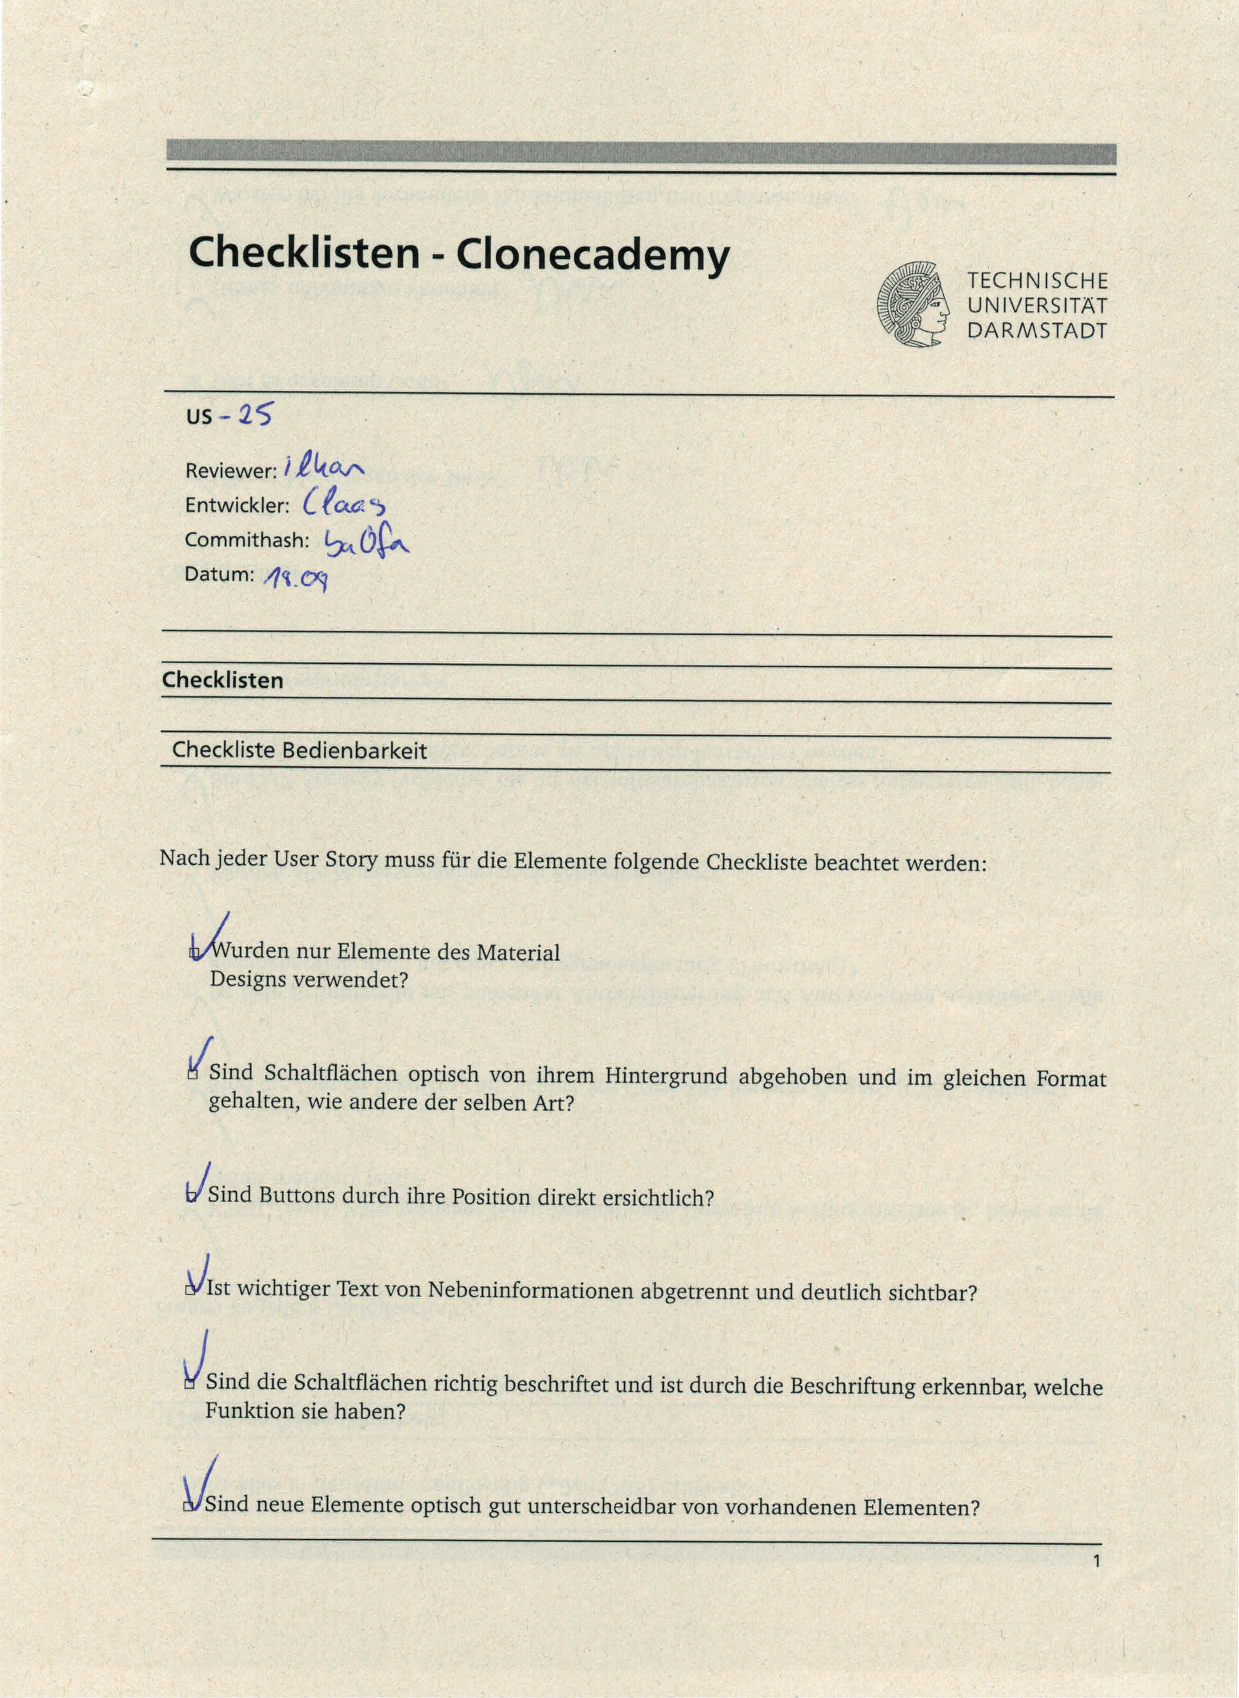
\includepdf[pages=-,pagecommand={},width=\textwidth]{appendix/checklisten/25_01.pdf}
	%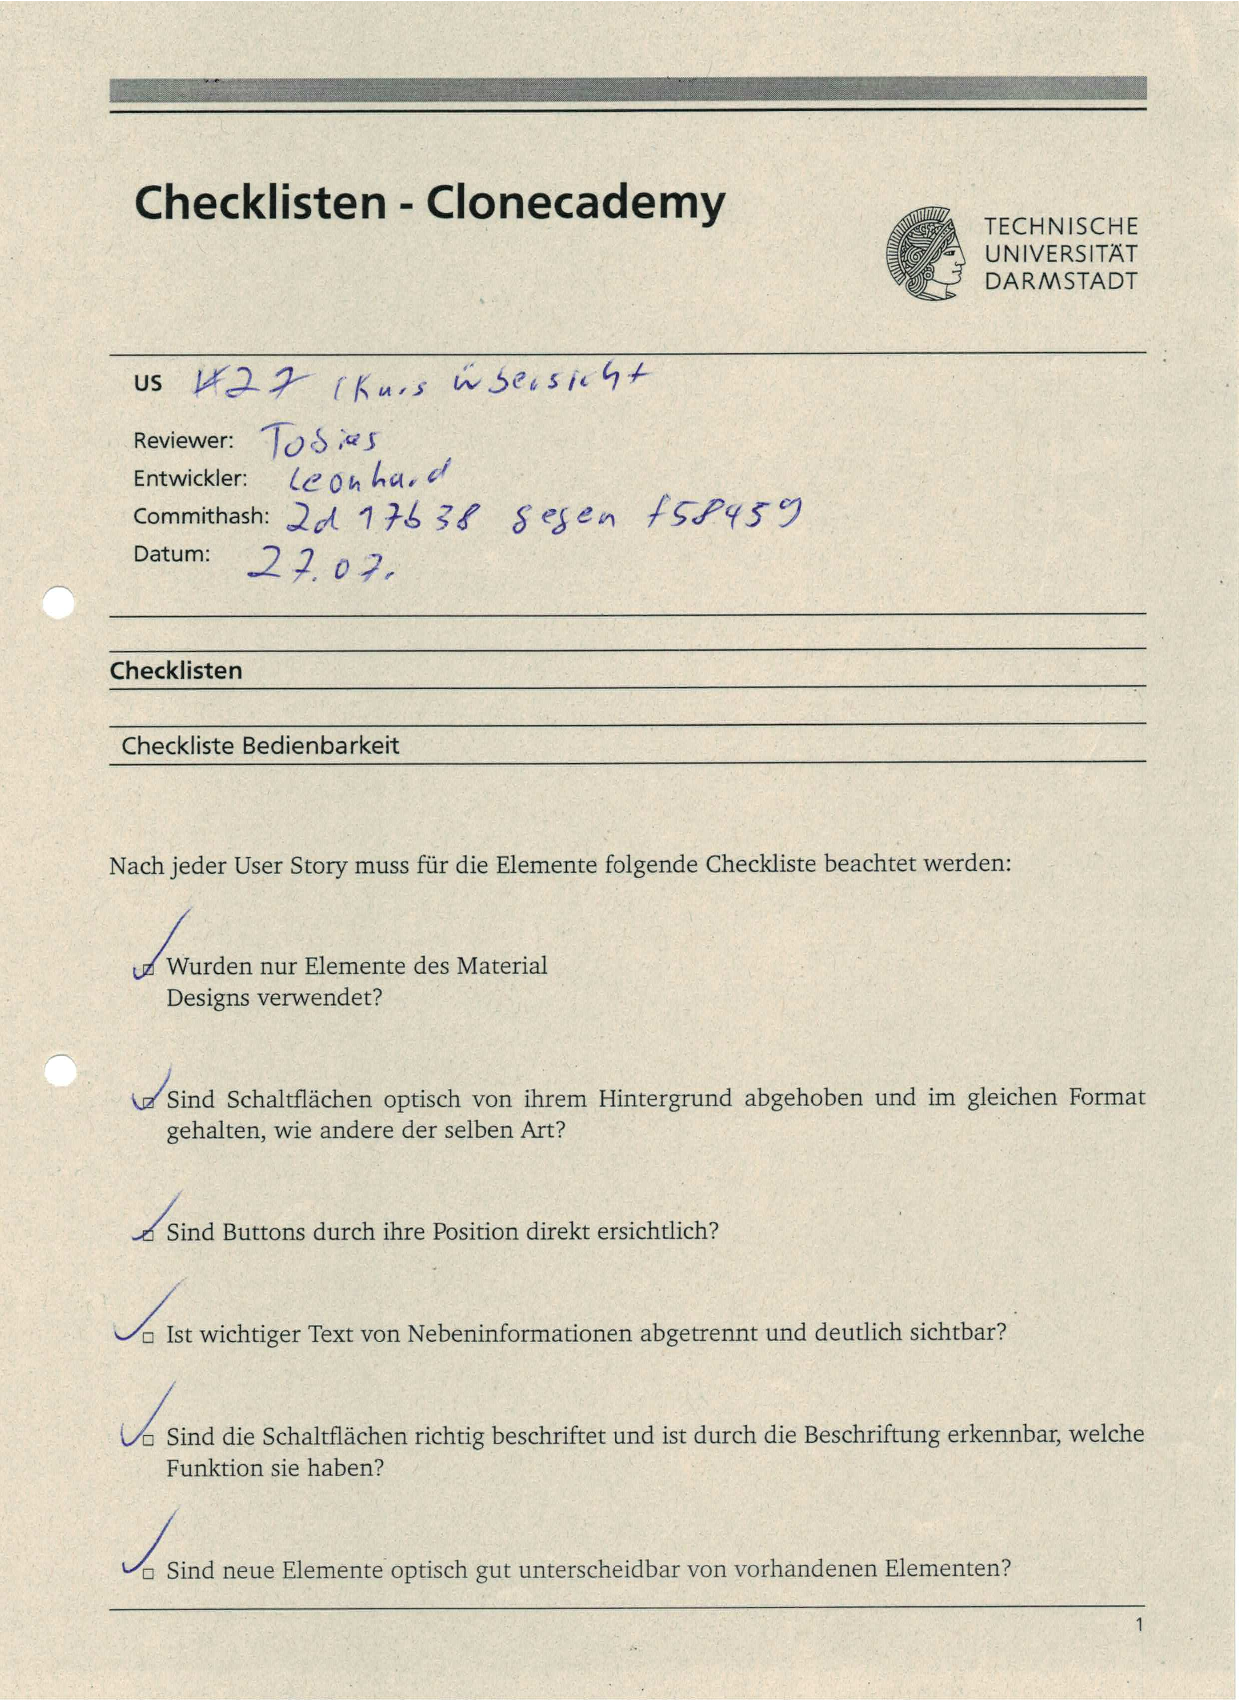
\includepdf[pages=-,pagecommand={},width=\textwidth]{appendix/checklisten/27_01.pdf}

\subsection{Veränderbarkeit}
\subsubsection{ng lint Output}
\lstinputlisting{appendix/ng_lint/ng_clean_14.txt}

\subsubsection{pylint Output}
\lstinputlisting{appendix/pylint/meldung_pylint_it14.txt}

\subsubsection{coverage Output}
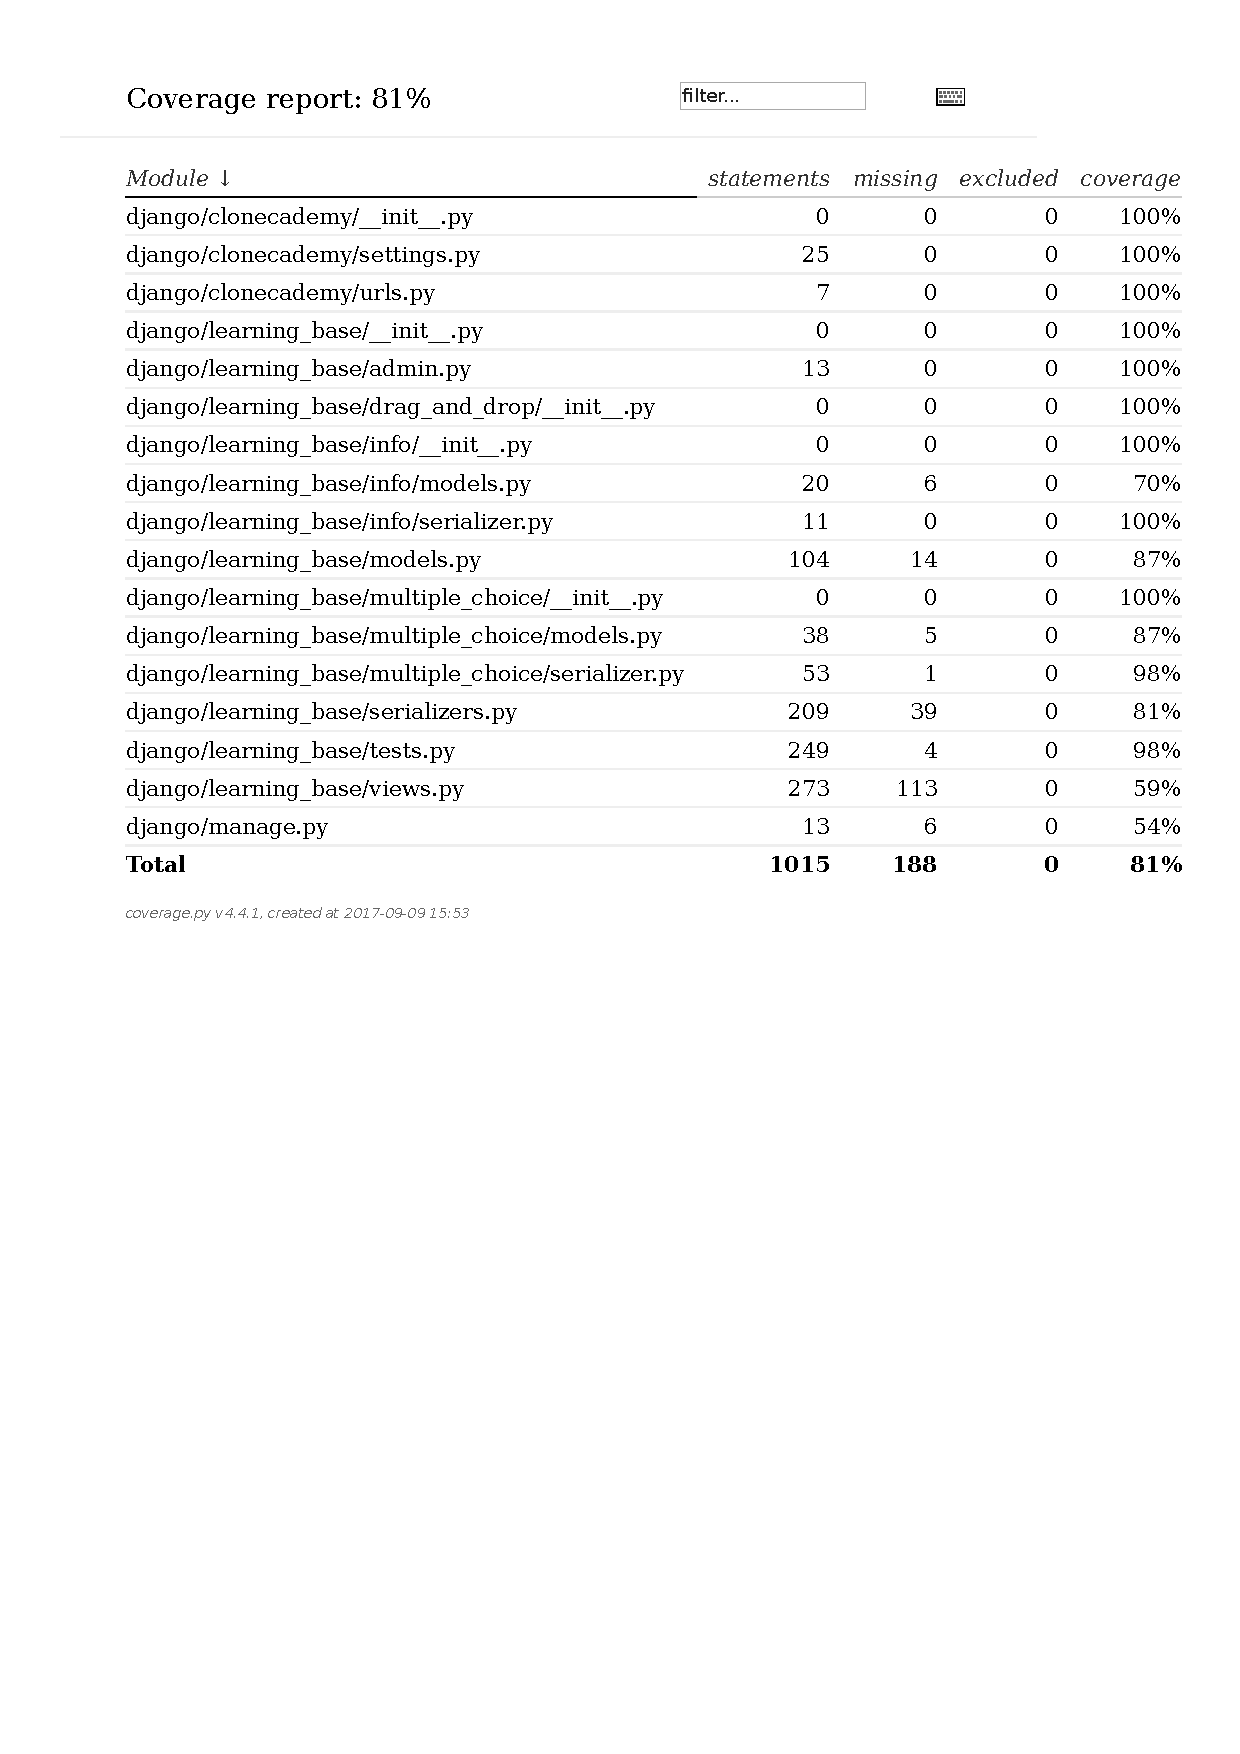
\includepdf[pages=-,pagecommand={},width=\textwidth]{appendix/coverage/django_test_14.pdf}

\subsection{Datensicherheit}
	\subsubsection{bandit Output}
	\lstinputlisting{appendix/bandit/bandit_ba0fa.txt}
	

\section{Iteration 15 - 24.08.}
	Abgegebene Userstories: 38
	
	Commit Hash: 78f8954ebc159fbcb6ed6a767e18d3437a604d22
	
	\subsection*{Checklisten}
	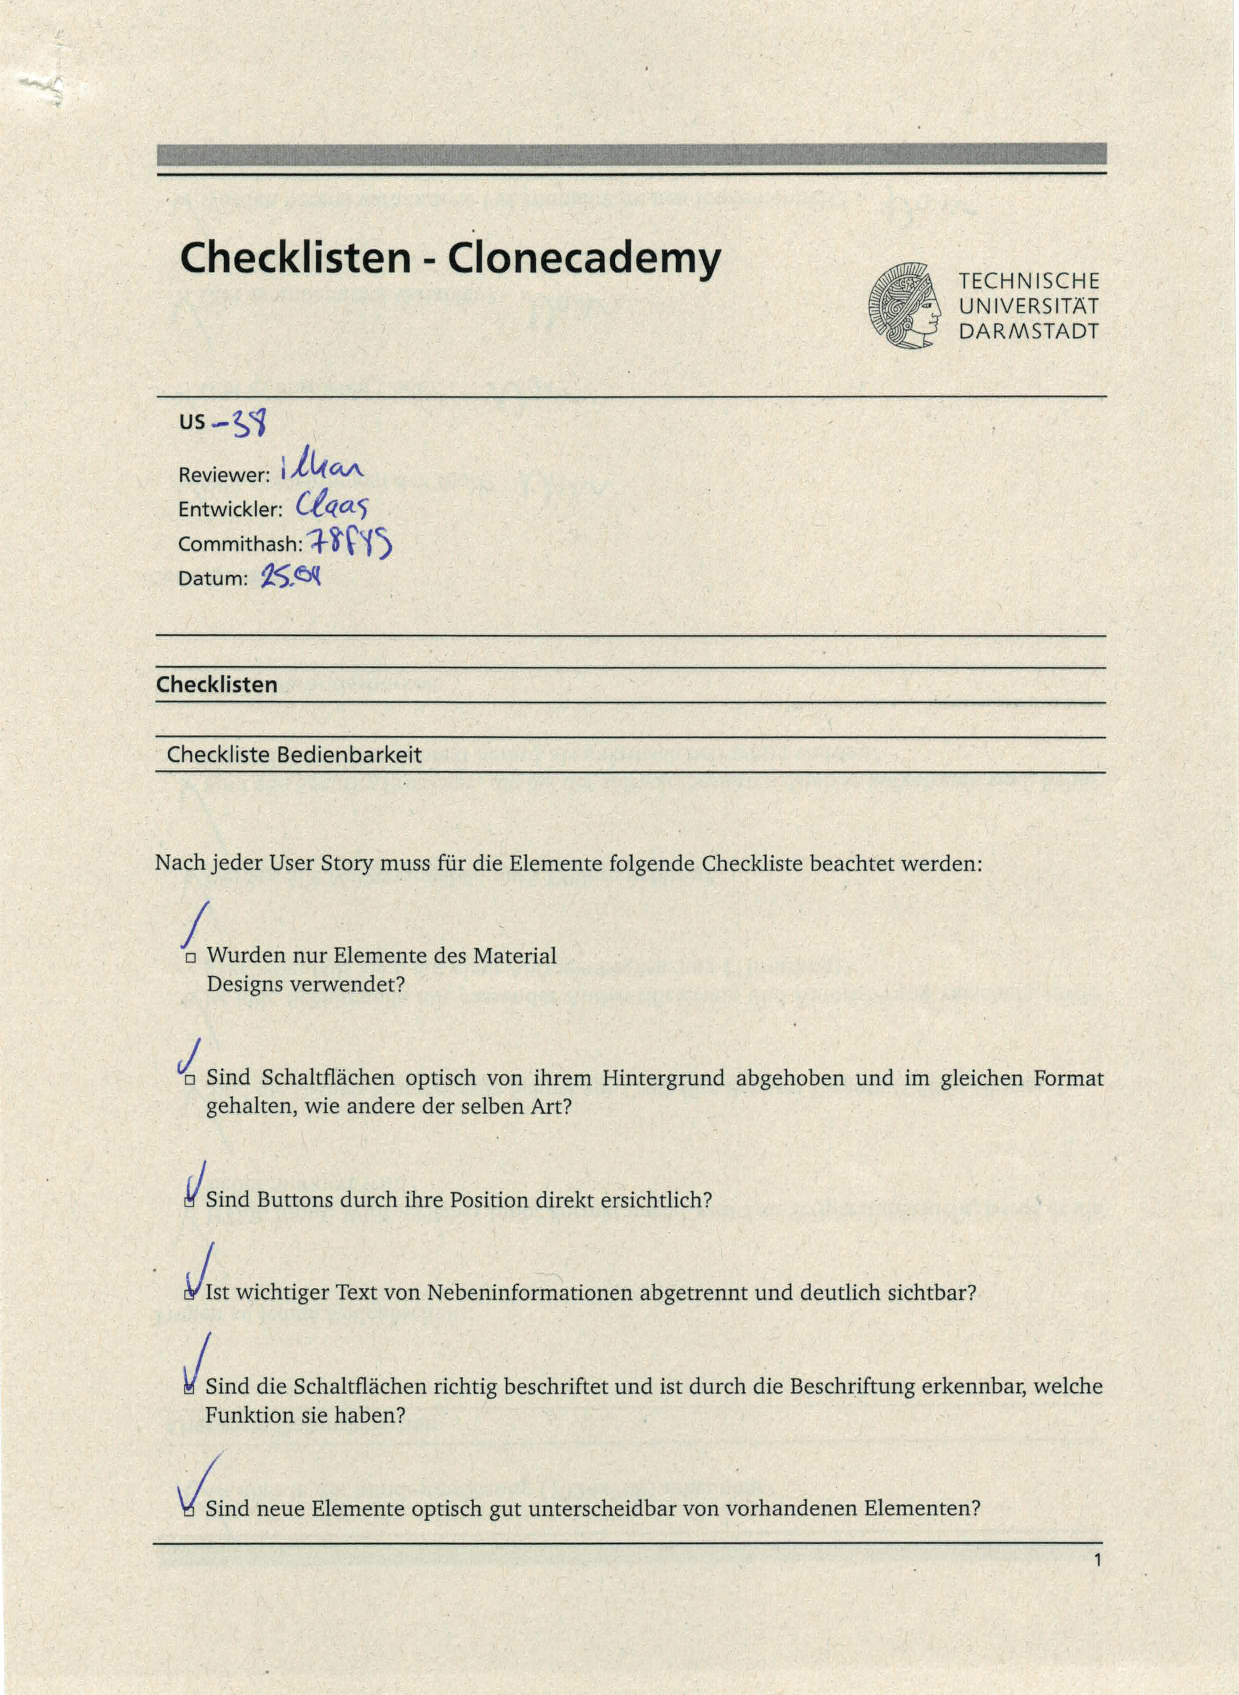
\includepdf[pages=-,pagecommand={},width=\textwidth]{appendix/checklisten/38_01.pdf}

	\subsection*{Veränderbarkeit}
	\subsubsection*{ng lint Output}
	\lstinputlisting{appendix/ng_lint/ng_clean_15.txt}

	\subsubsection*{pylint Output}
	\lstinputlisting{appendix/pylint/meldung_pylint_it15.txt}

	\subsubsection*{coverage Output}
	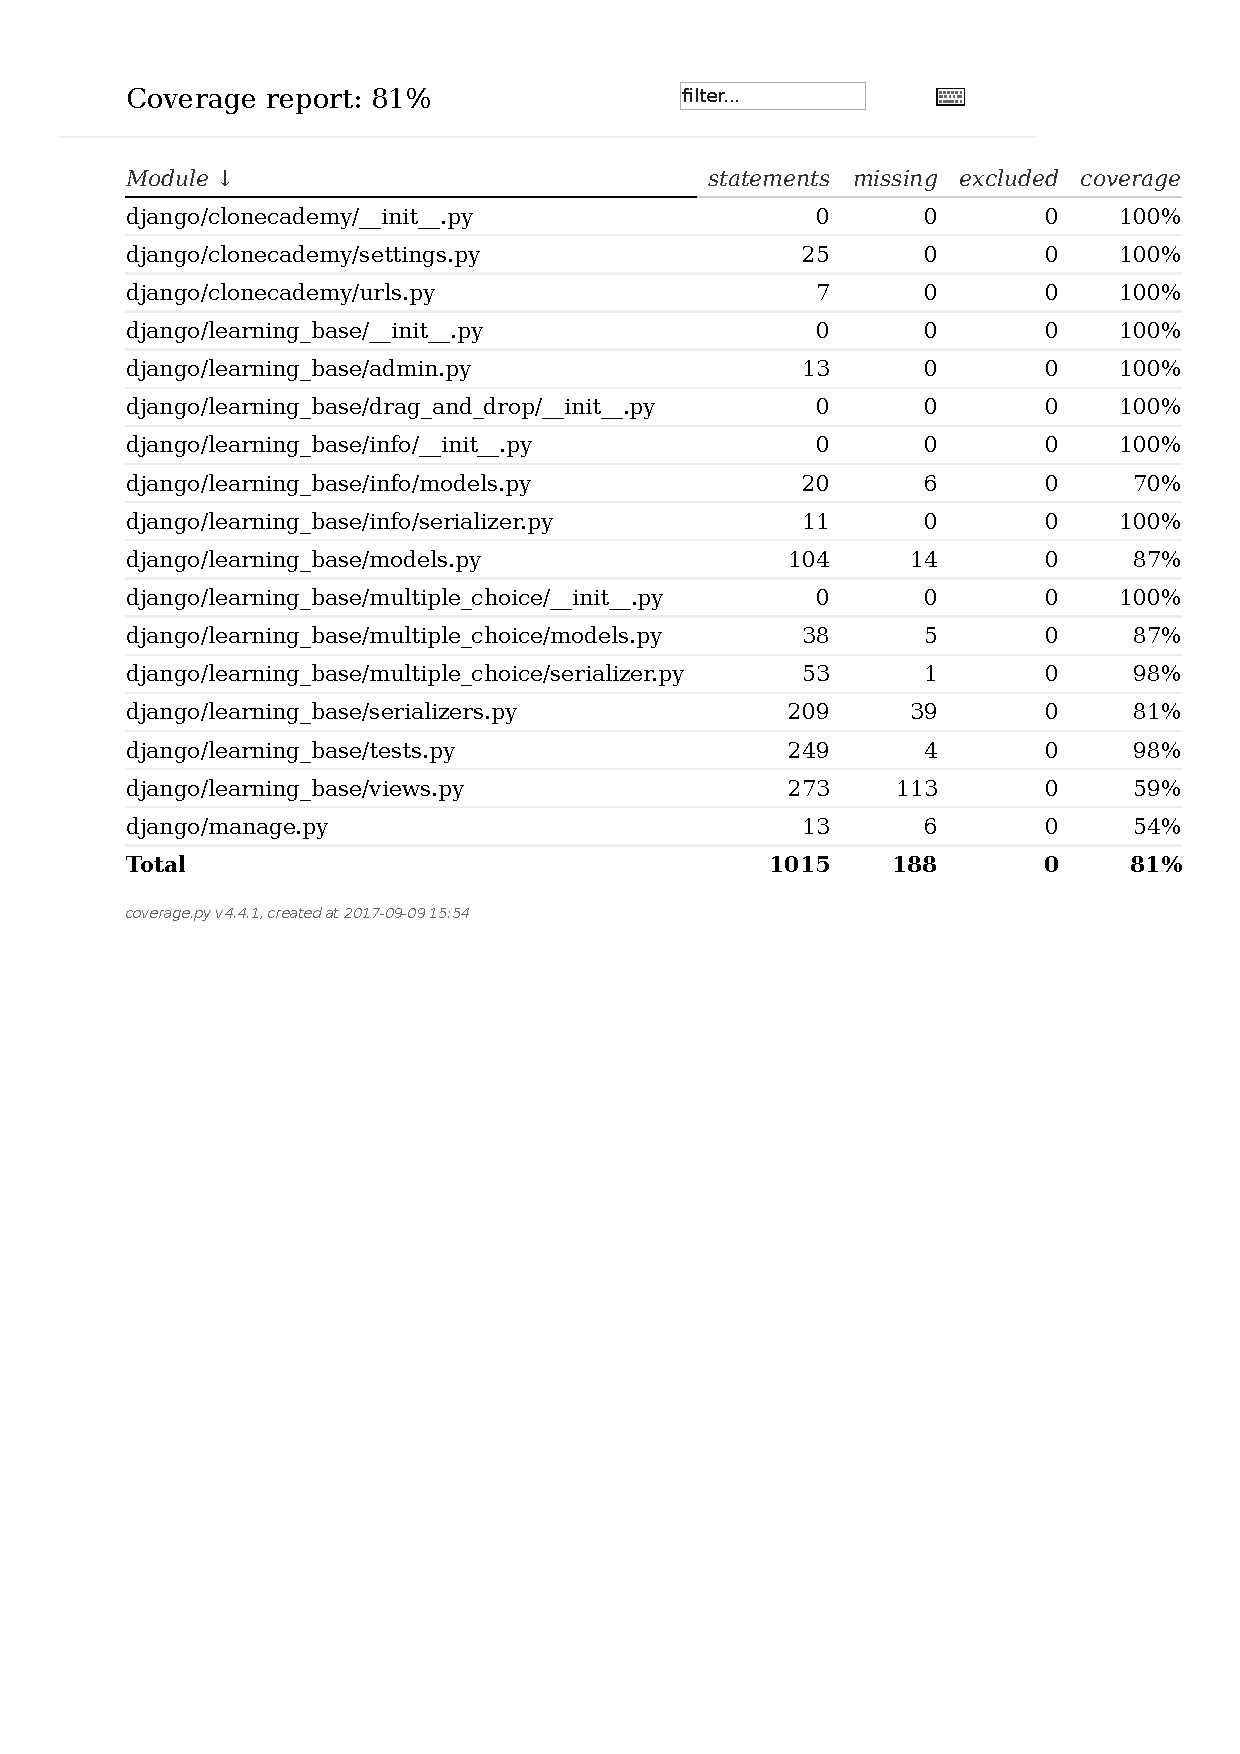
\includepdf[pages=-,pagecommand={},width=\textwidth]{appendix/coverage/django_test_15.pdf}

	\subsection*{Datensicherheit}
	\subsubsection*{bandit Output}
	\lstinputlisting{appendix/bandit/bandit_78f89.txt}

\section{Iteration 16 - 31.08.} 
	Abgegebene Userstories: 30, 32, 36, 37, 40, 41
	
	Commit Hash: 11bc7fa37a20ac045d5a6c29e4e3a060b73b3504
	
	\subsection{Checklisten}
	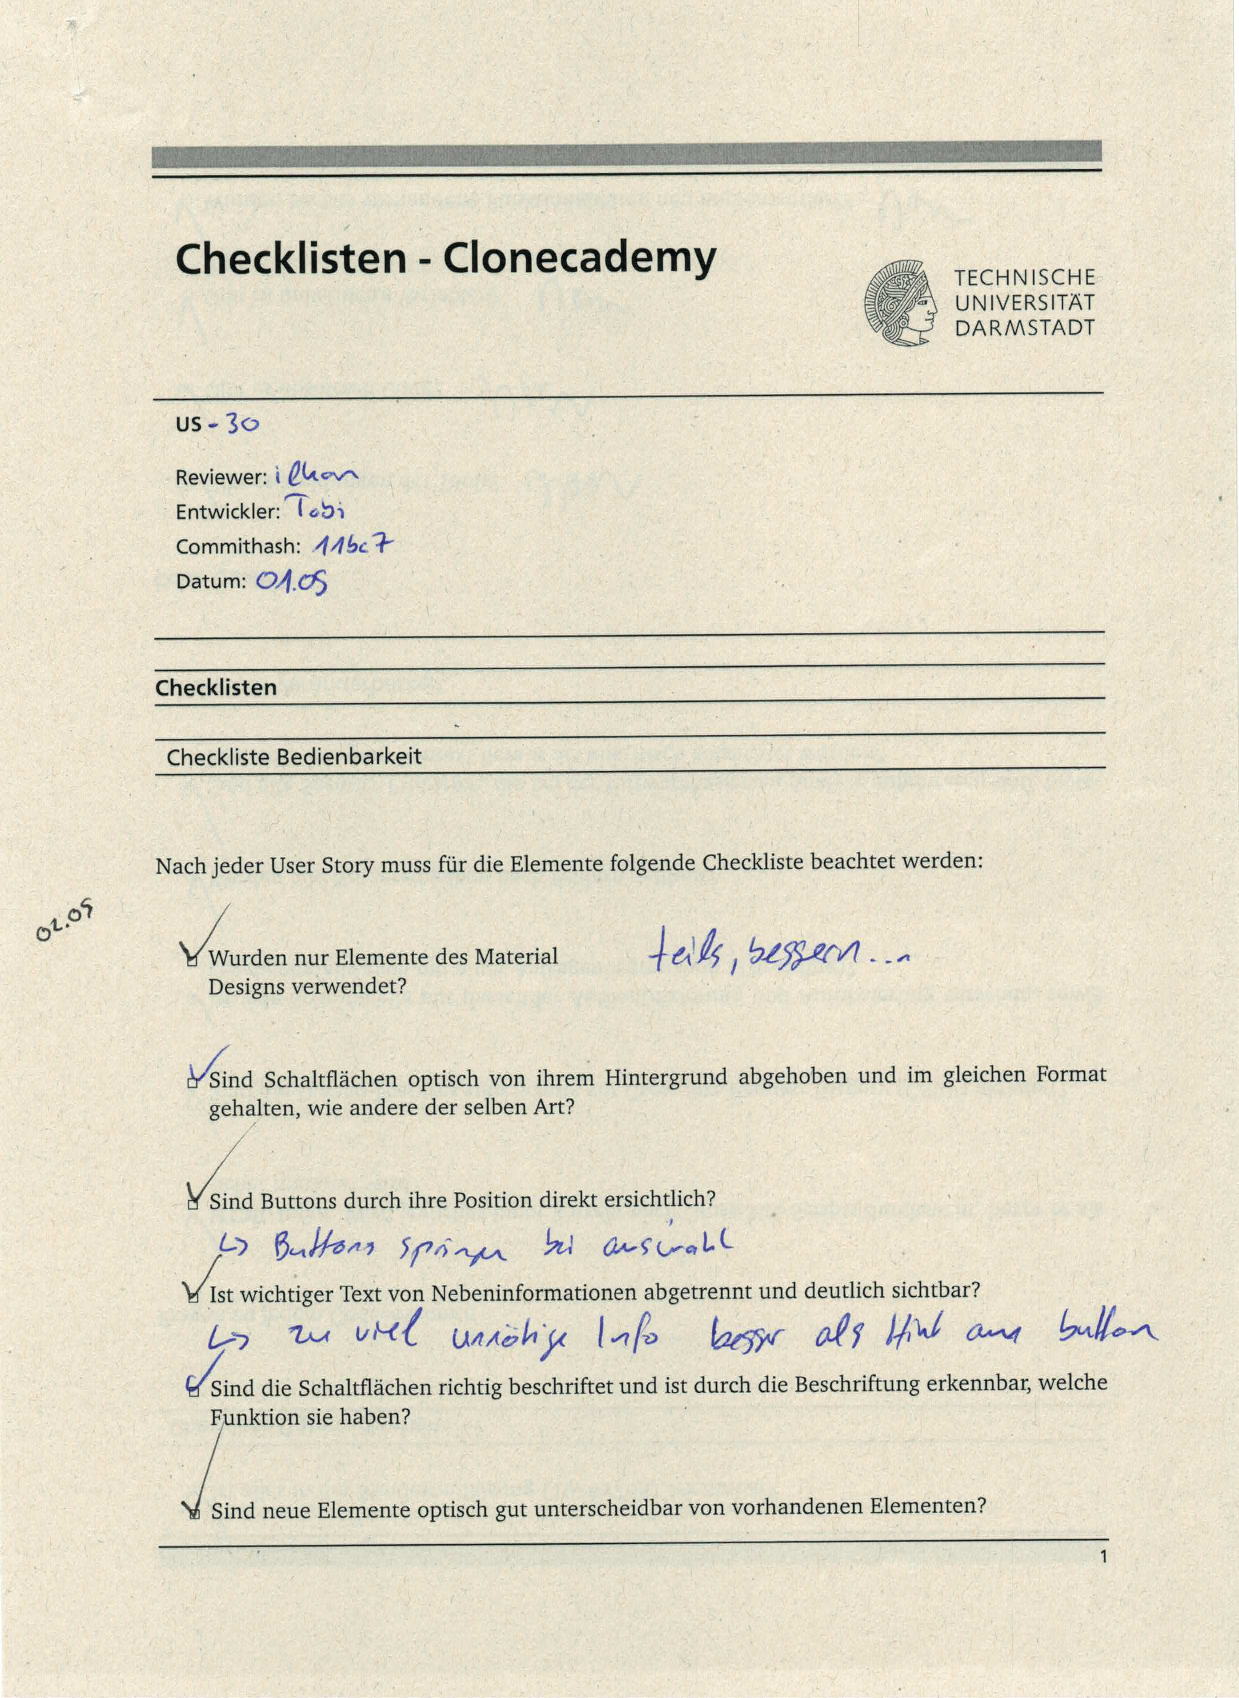
\includepdf[pages=-,pagecommand={},width=\textwidth]{appendix/checklisten/30_01.pdf}
	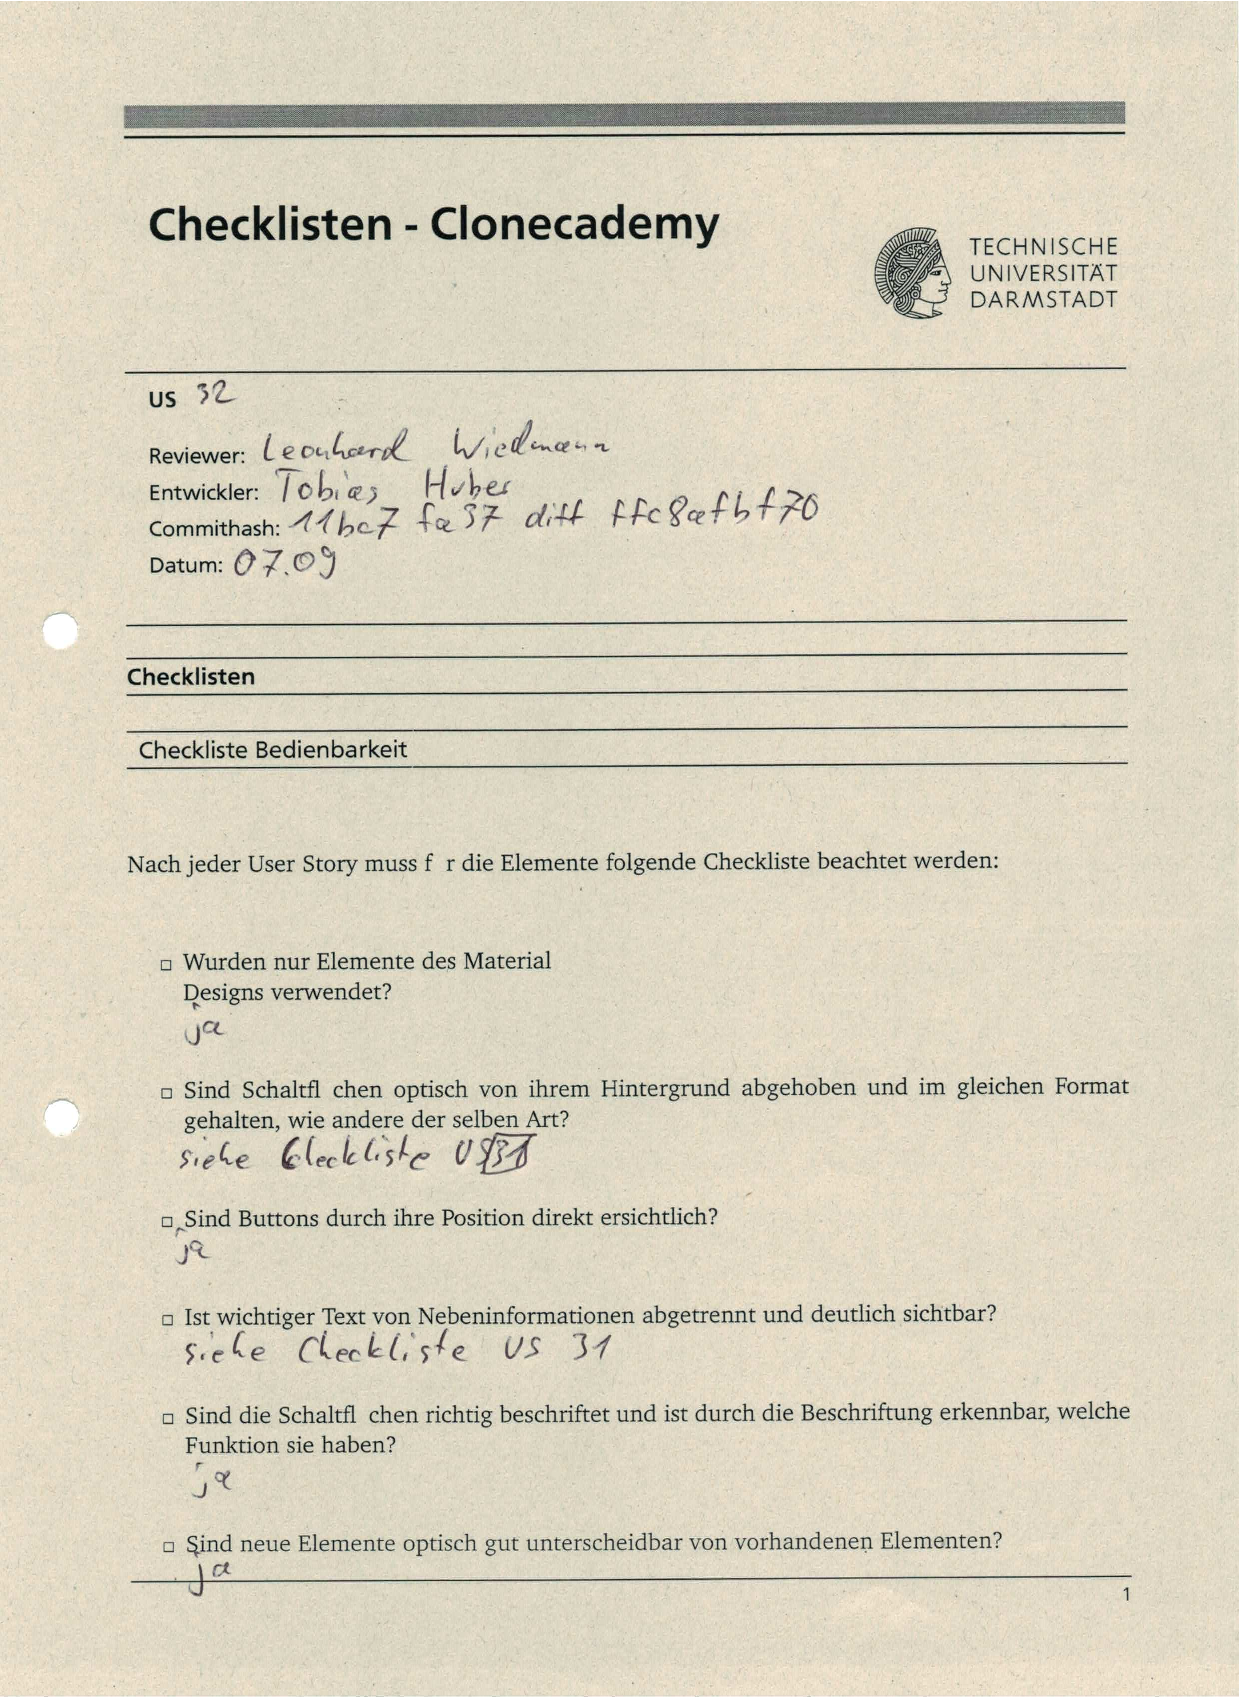
\includepdf[pages=-,pagecommand={},width=\textwidth]{appendix/checklisten/32_01.pdf}
	%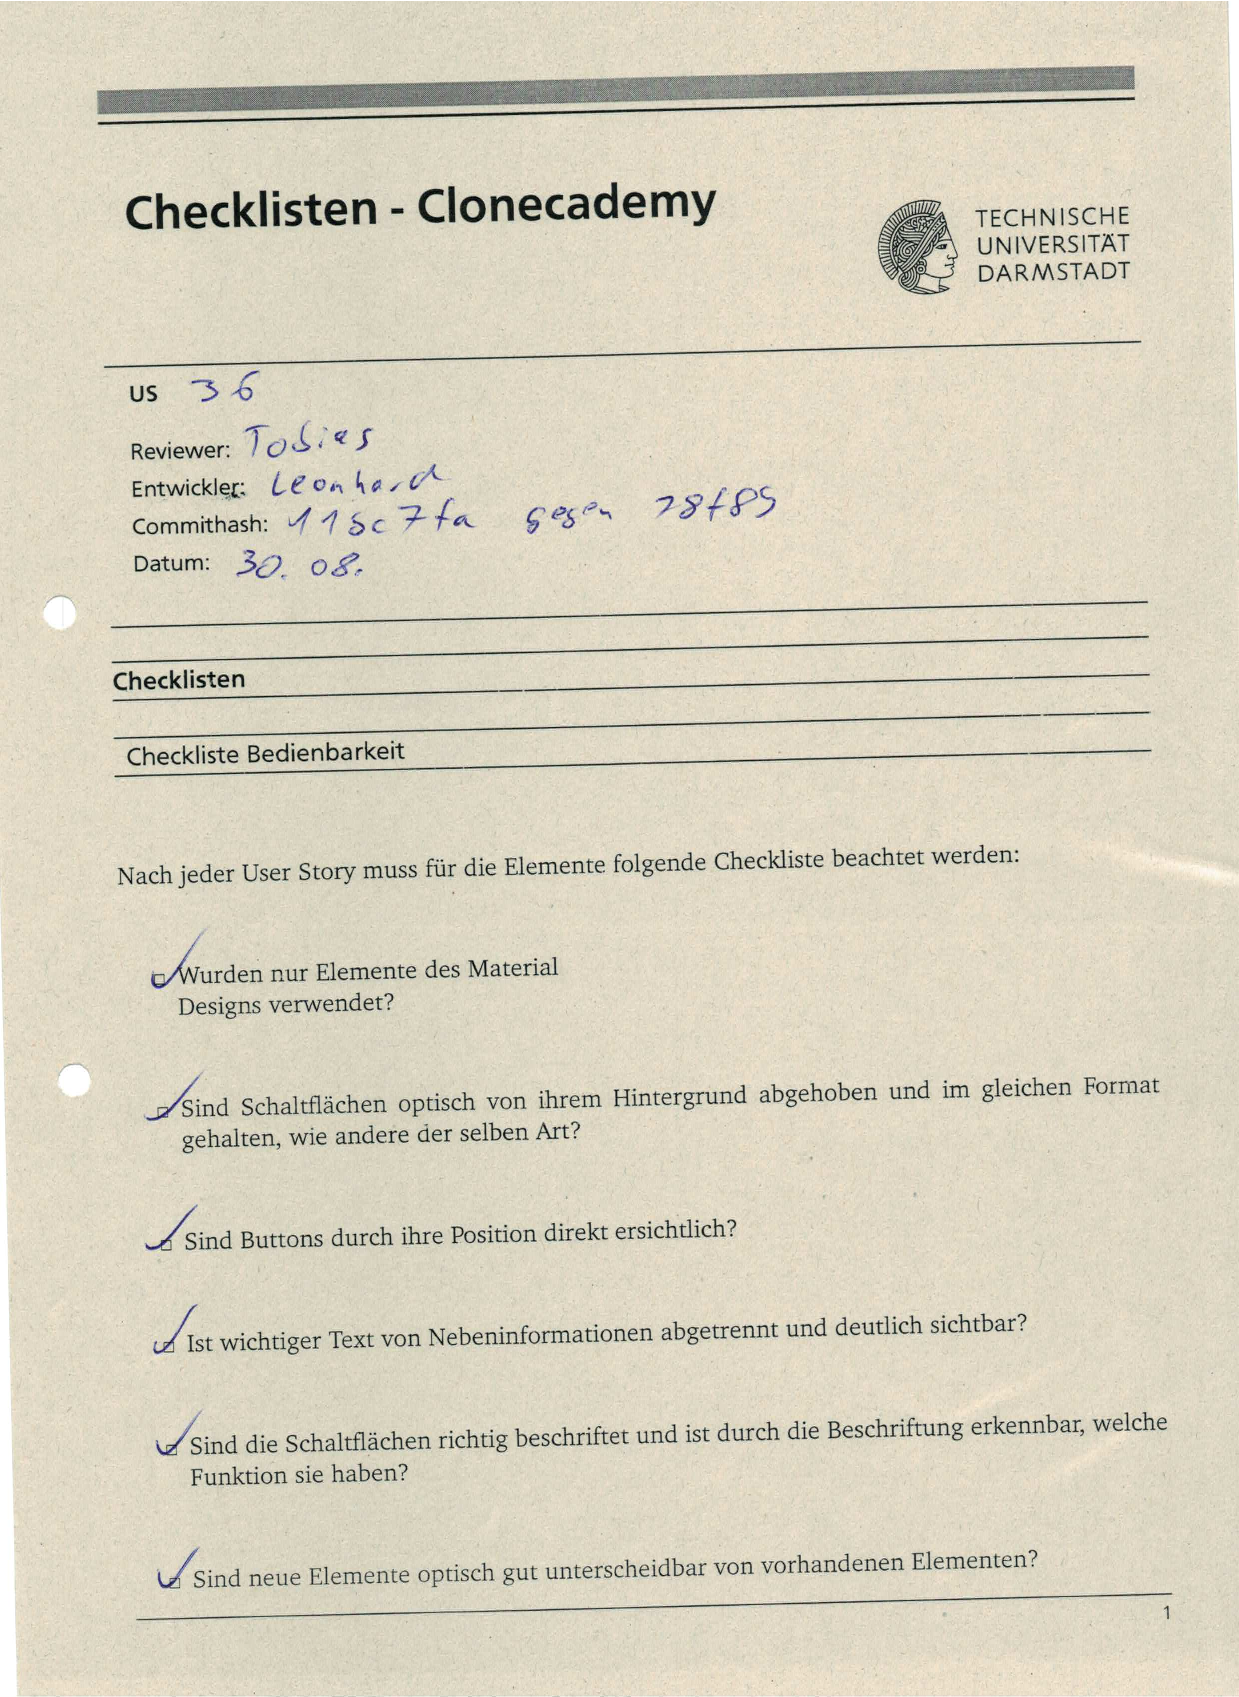
\includepdf[pages=-,pagecommand={},width=\textwidth]{appendix/checklisten/36_01.pdf}
	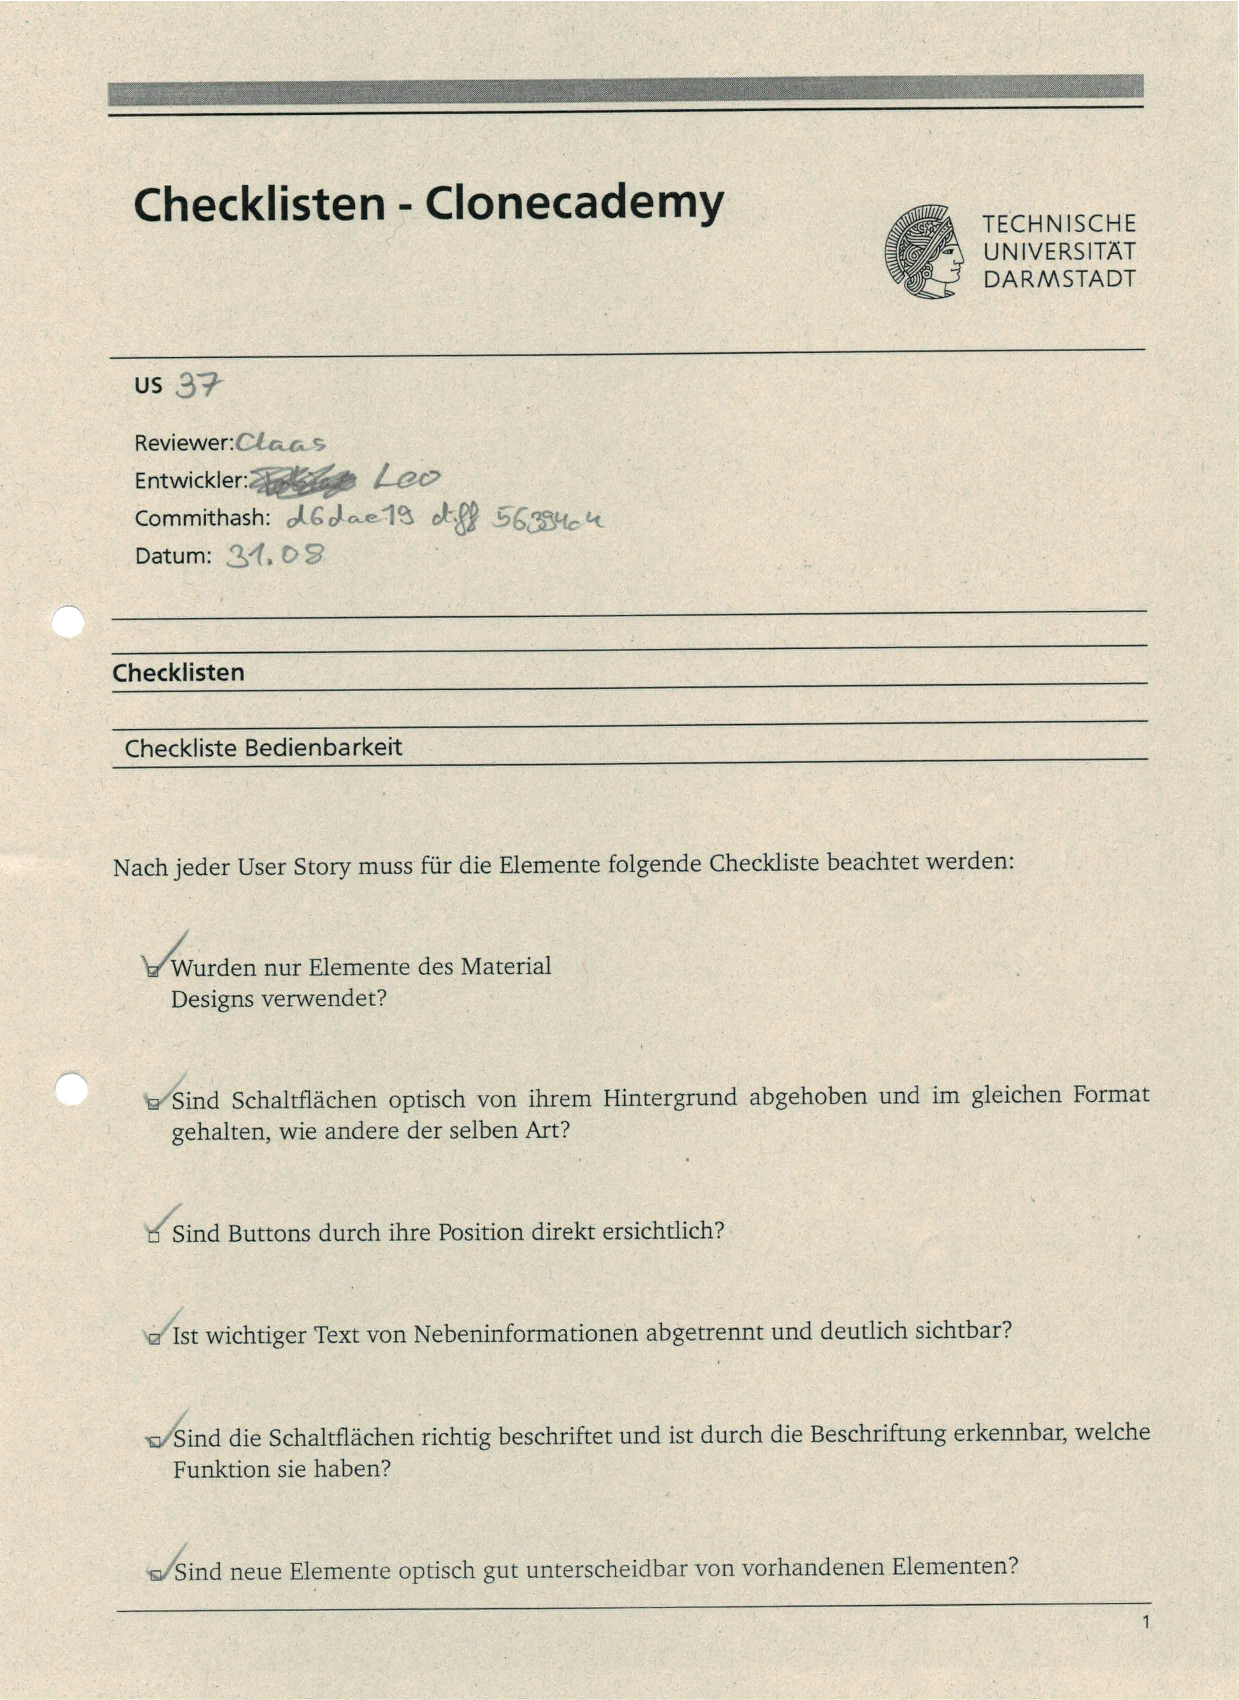
\includepdf[pages=-,pagecommand={},width=\textwidth]{appendix/checklisten/37_01.pdf}
	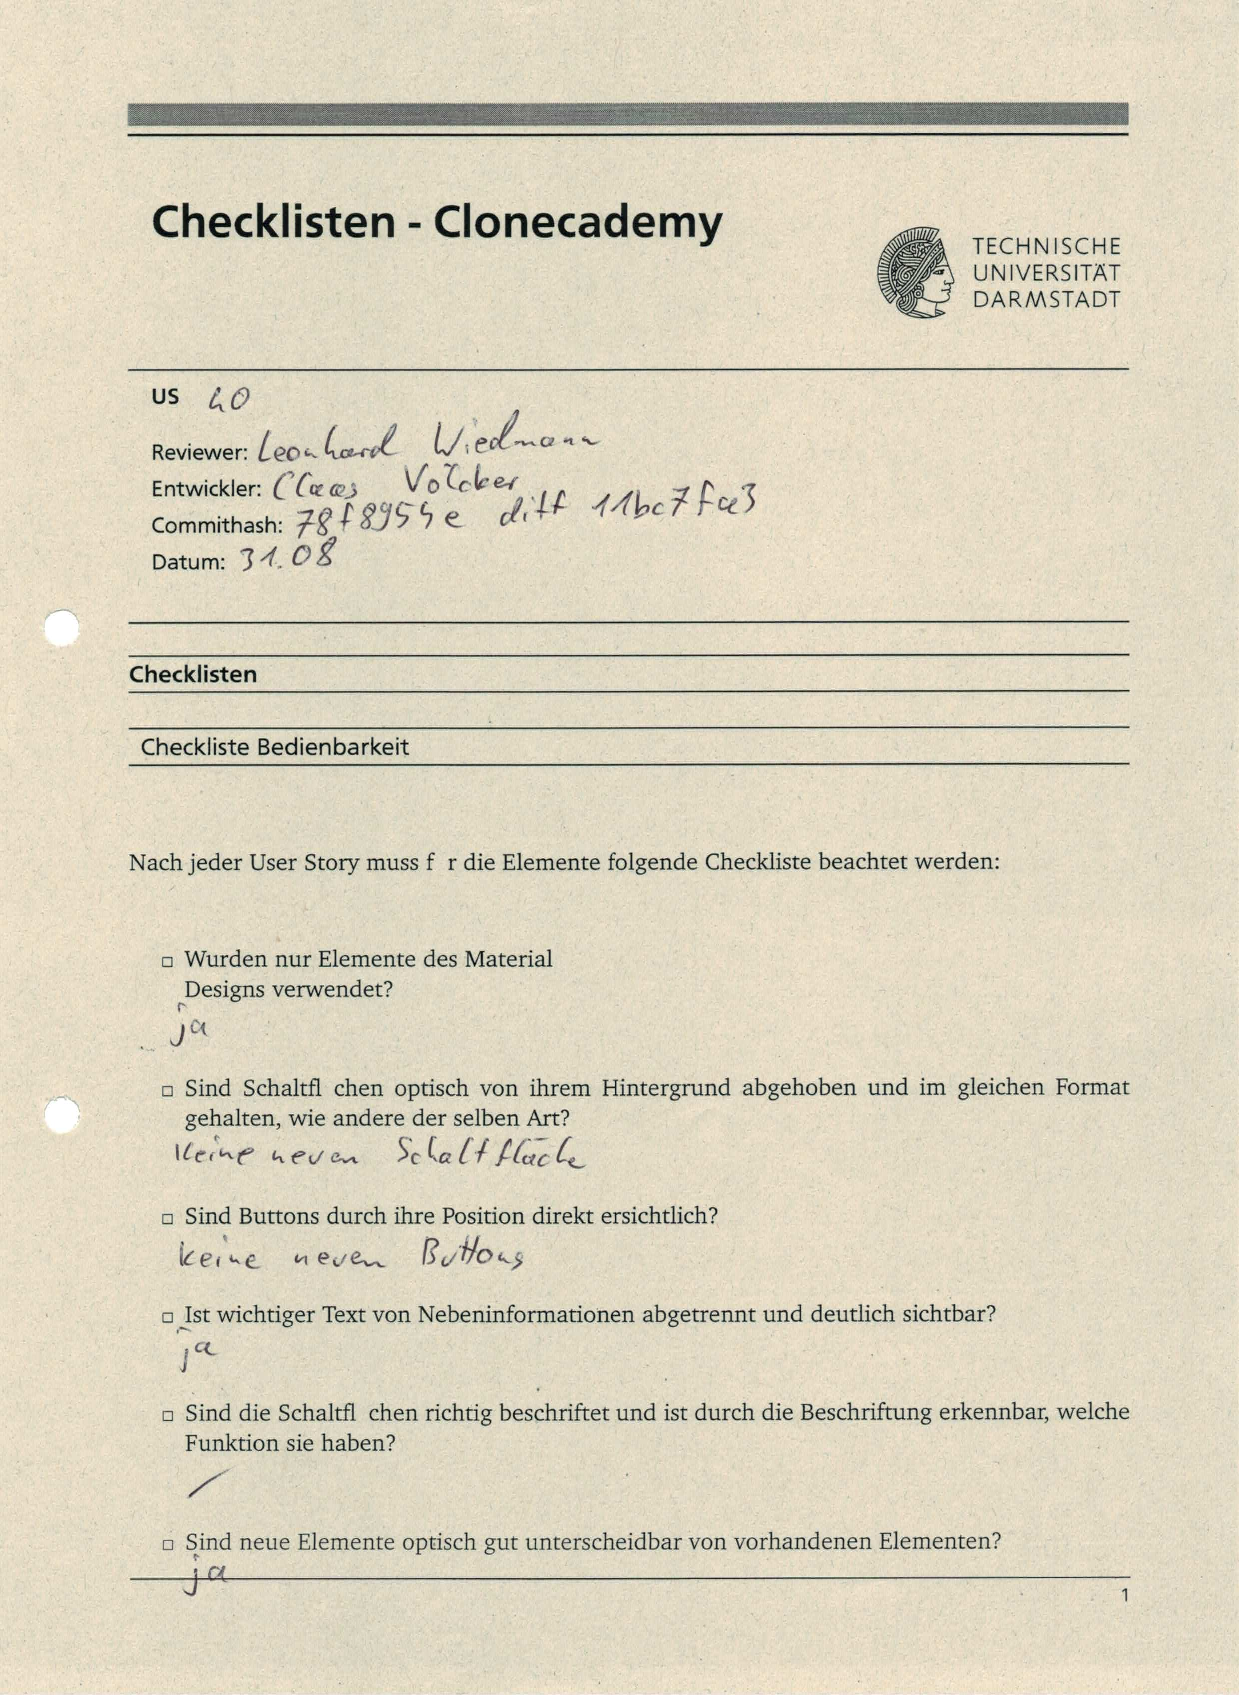
\includepdf[pages=-,pagecommand={},width=\textwidth]{appendix/checklisten/40_01.pdf}
	%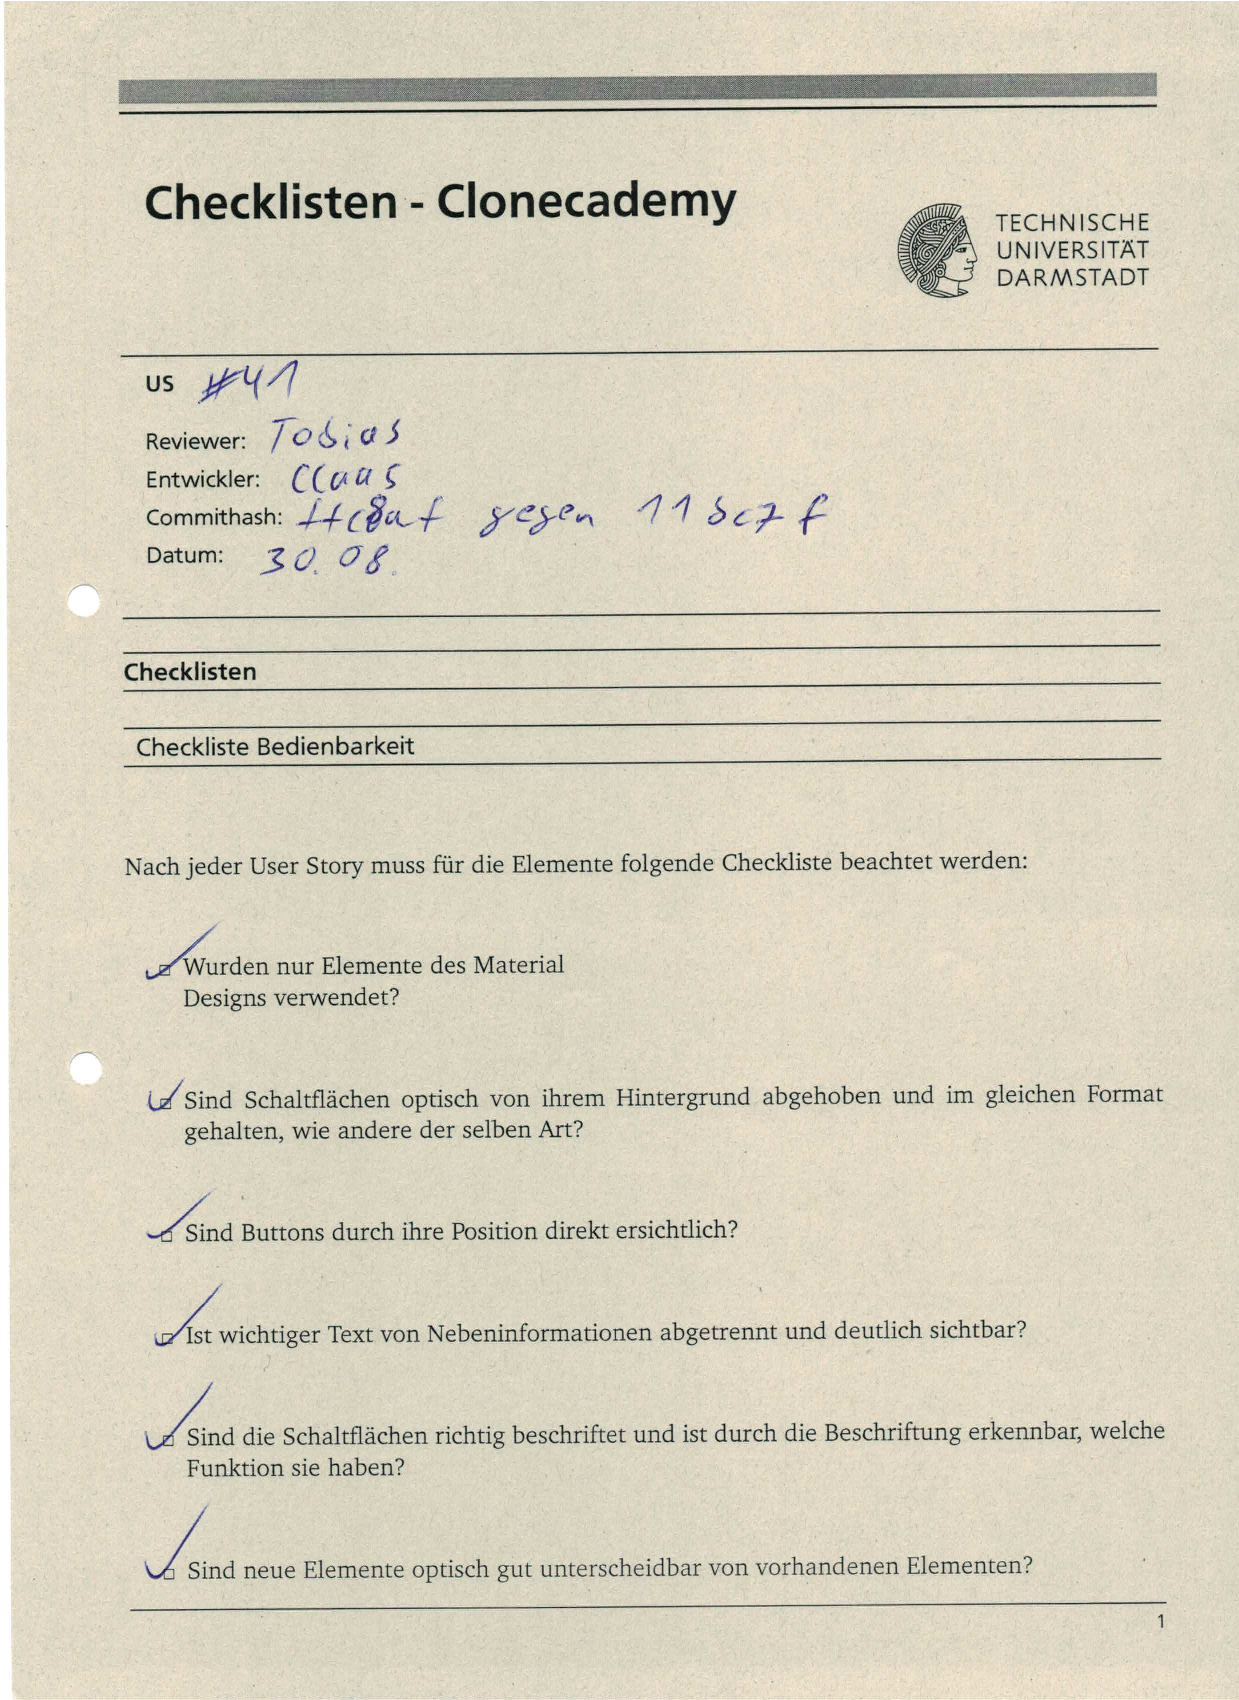
\includepdf[pages=-,pagecommand={},width=\textwidth]{appendix/checklisten/41_01.pdf}

	\subsection{Veränderbarkeit}
	\subsubsection{ng lint Output}
	\lstinputlisting{appendix/ng_lint/ng_clean_16.txt}

	\subsubsection{pylint Output}
	\lstinputlisting{appendix/pylint/meldung_pylint_it16.txt}

	\subsubsection{coverage Output}
	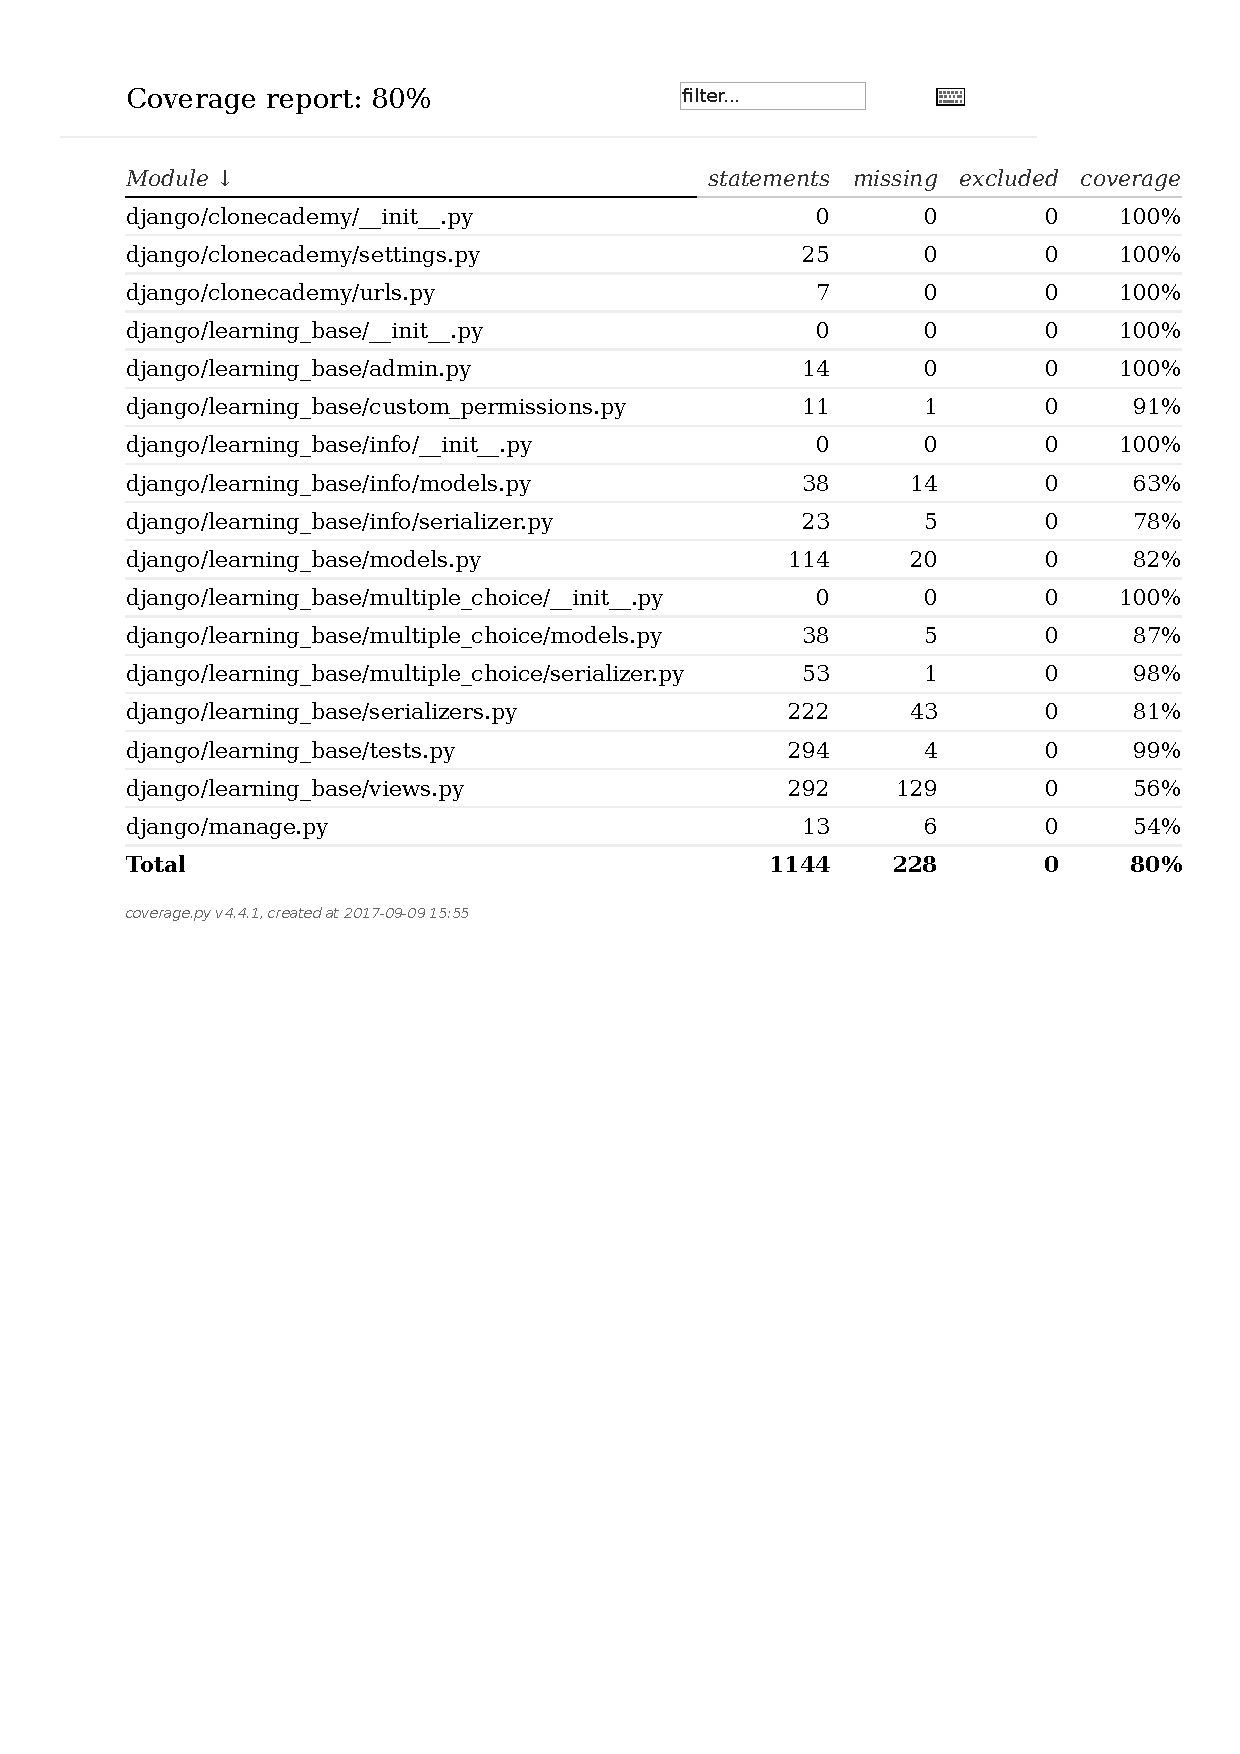
\includepdf[pages=-,pagecommand={},width=\textwidth]{appendix/coverage/django_test_16.pdf}

	\subsection{Datensicherheit}
	\subsubsection{bandit Output}
	\lstinputlisting{appendix/bandit/bandit_11bc7.txt}
\section{Iteration 17 - 07.09.}
	Abgegebene Userstories: 31, 33, 34, 42, 43, 44, 46
	
	Commit Hash: ffc8afbf7012f4b2d63e5b58ac8f0c224a7ee382
	
	\subsection*{Checklisten}
	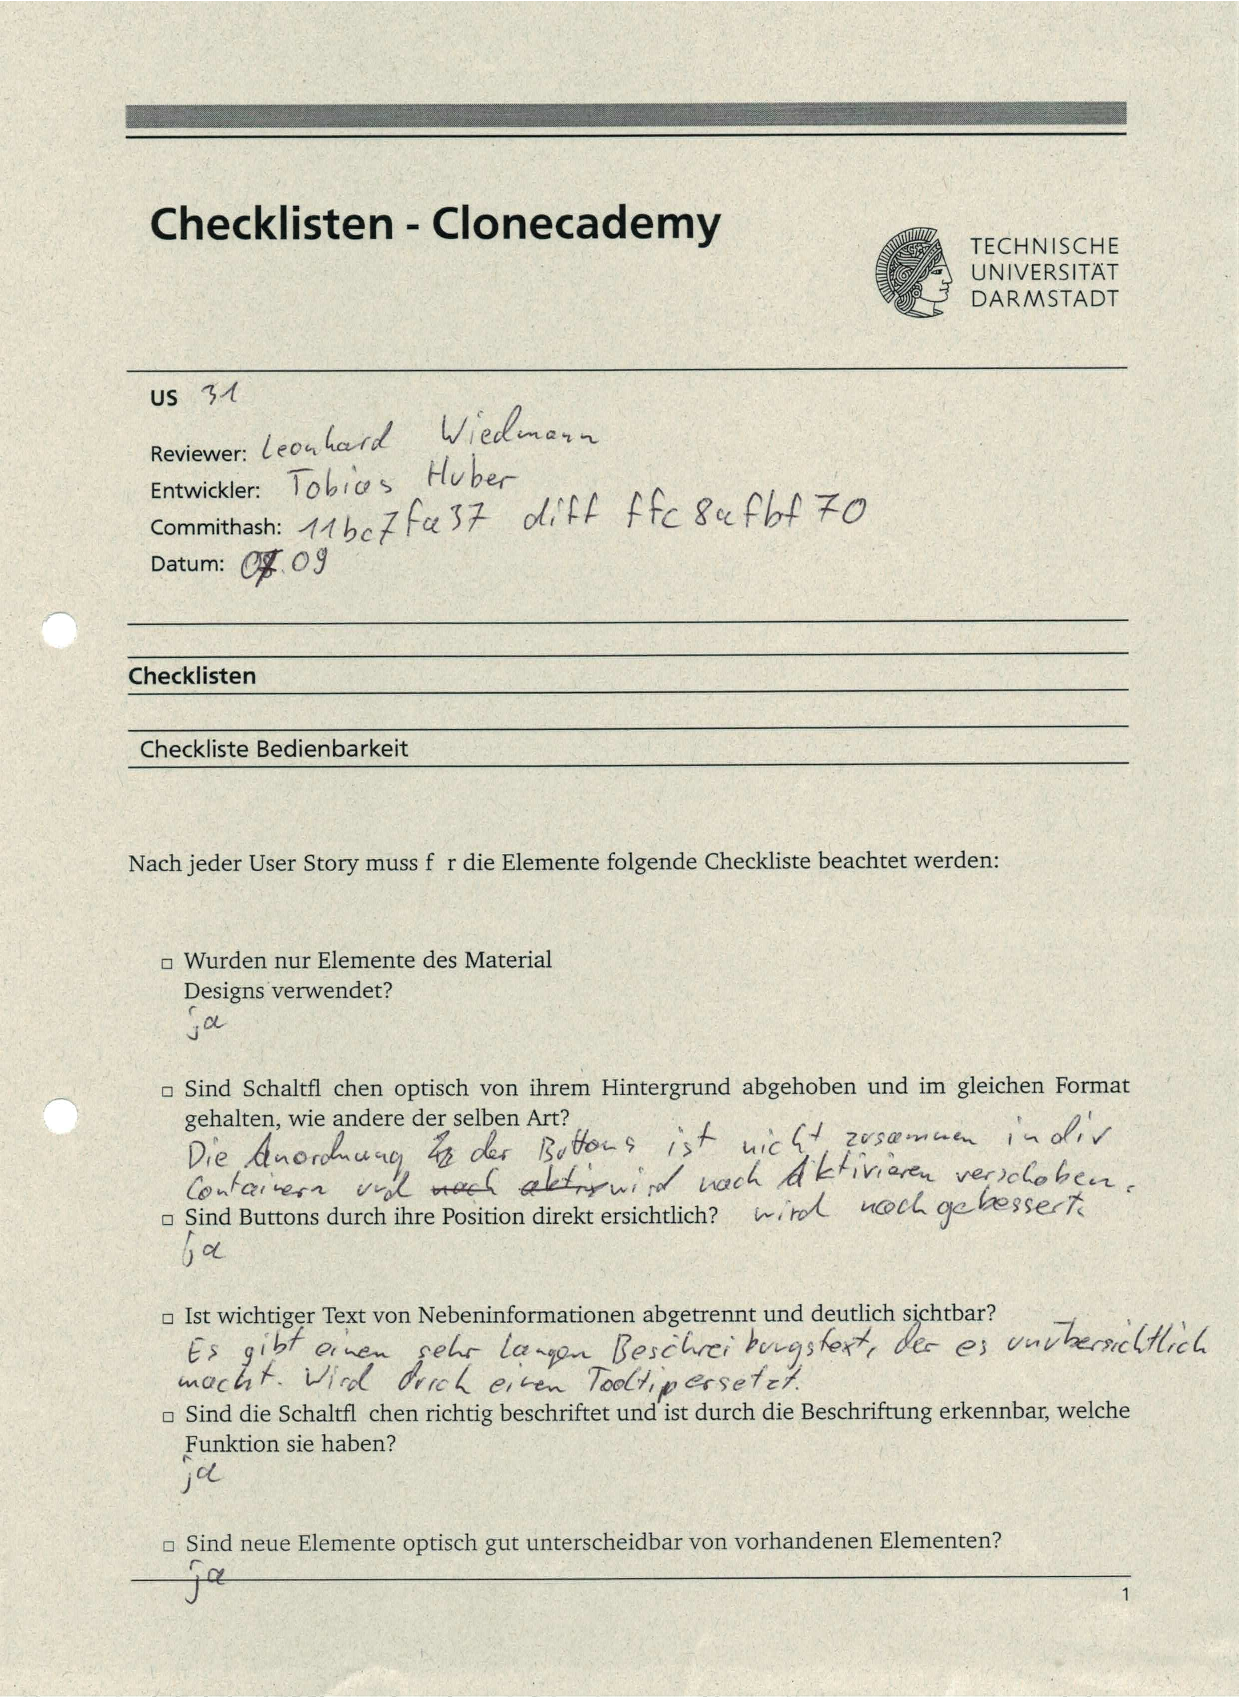
\includepdf[pages=-,pagecommand={},width=\textwidth]{appendix/checklisten/31_01.pdf}
	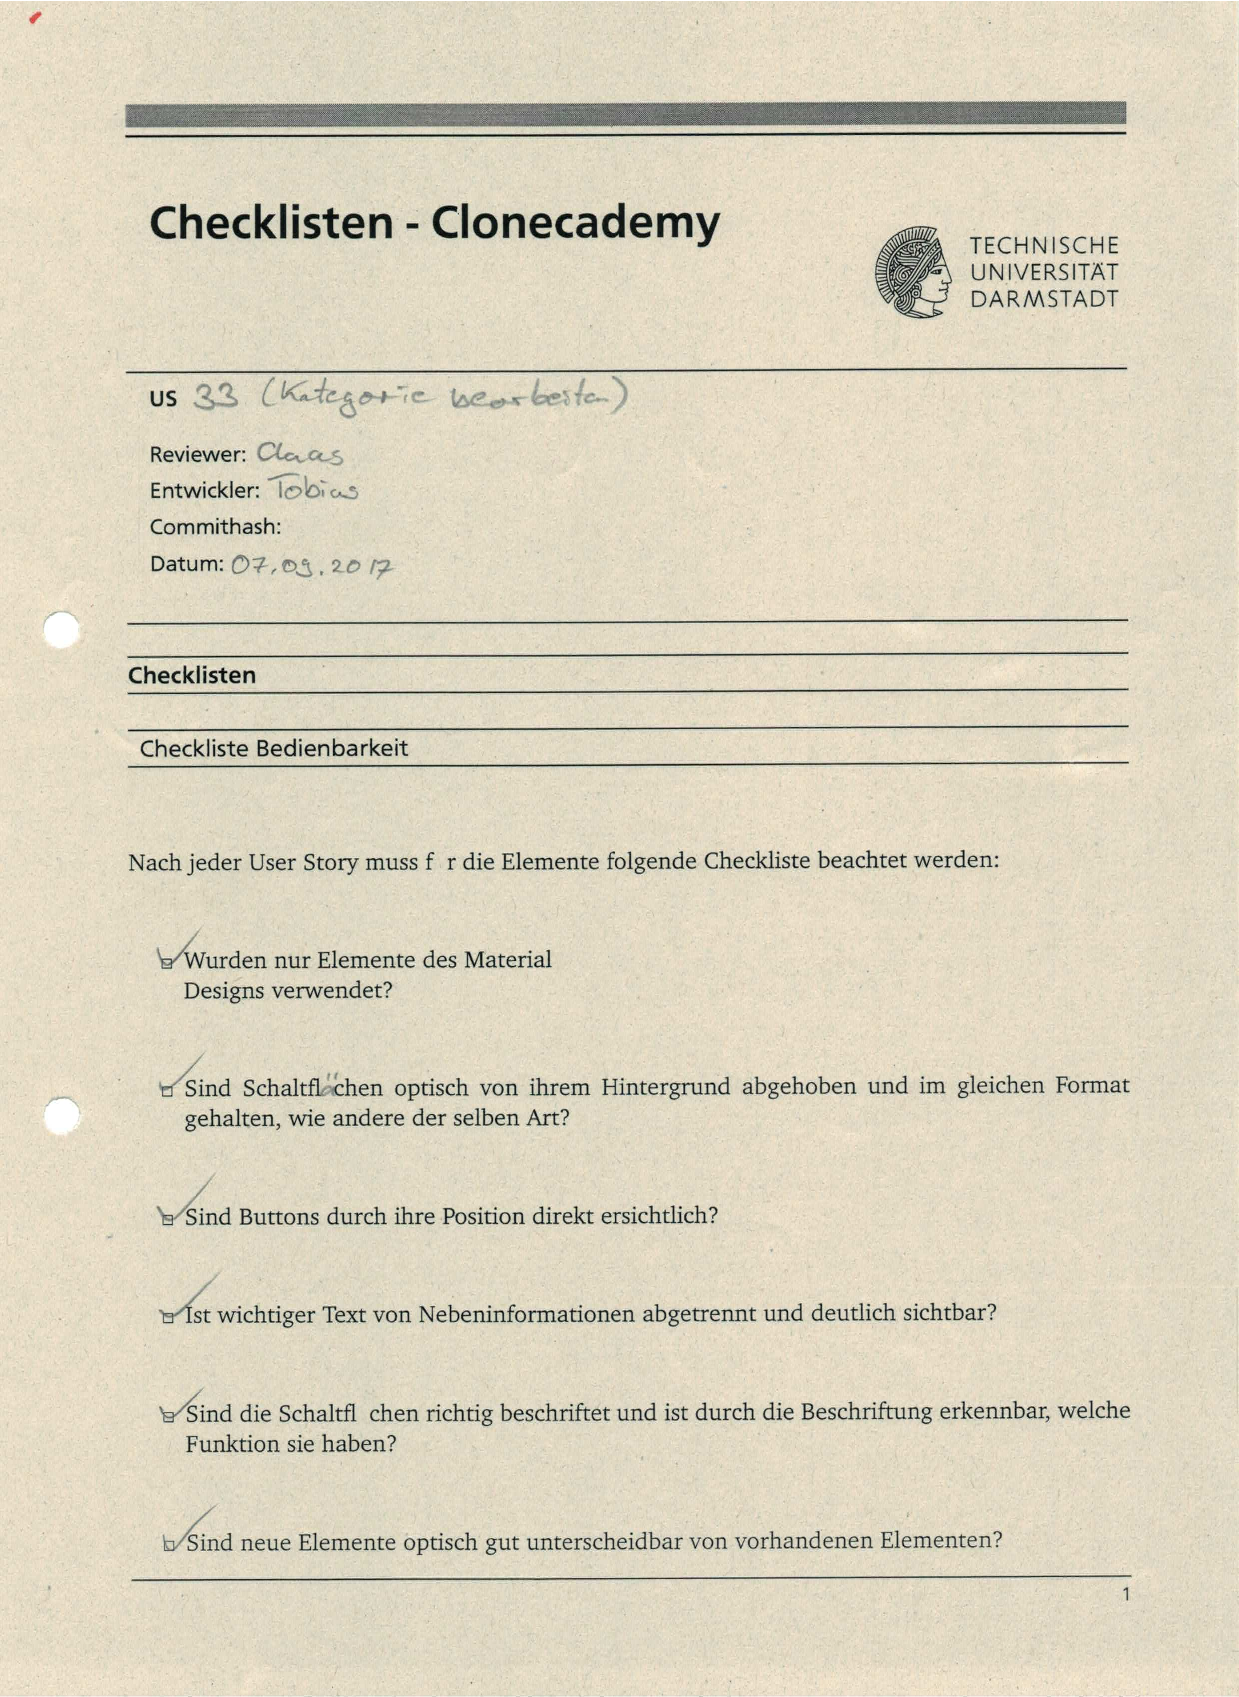
\includepdf[pages=-,pagecommand={},width=\textwidth]{appendix/checklisten/33_01.pdf}
	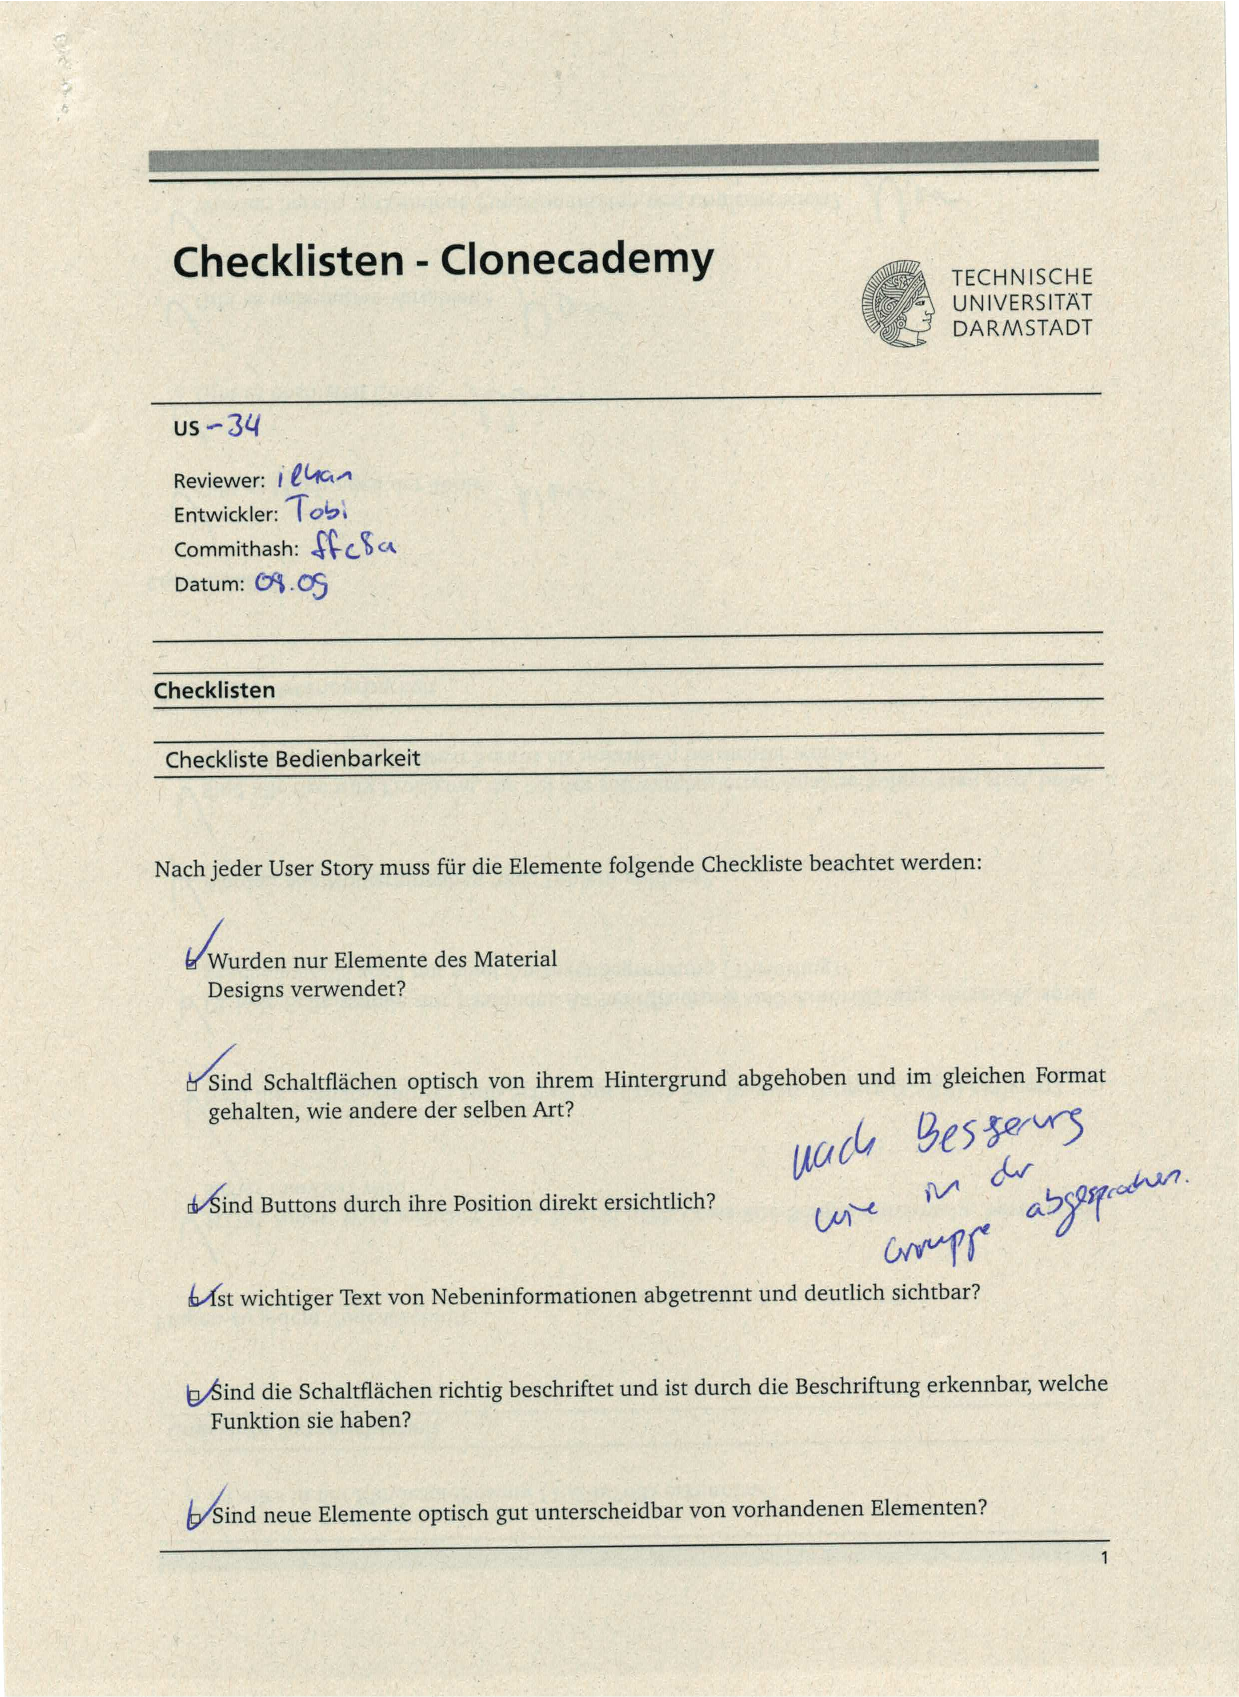
\includepdf[pages=-,pagecommand={},width=\textwidth]{appendix/checklisten/34_01.pdf}
	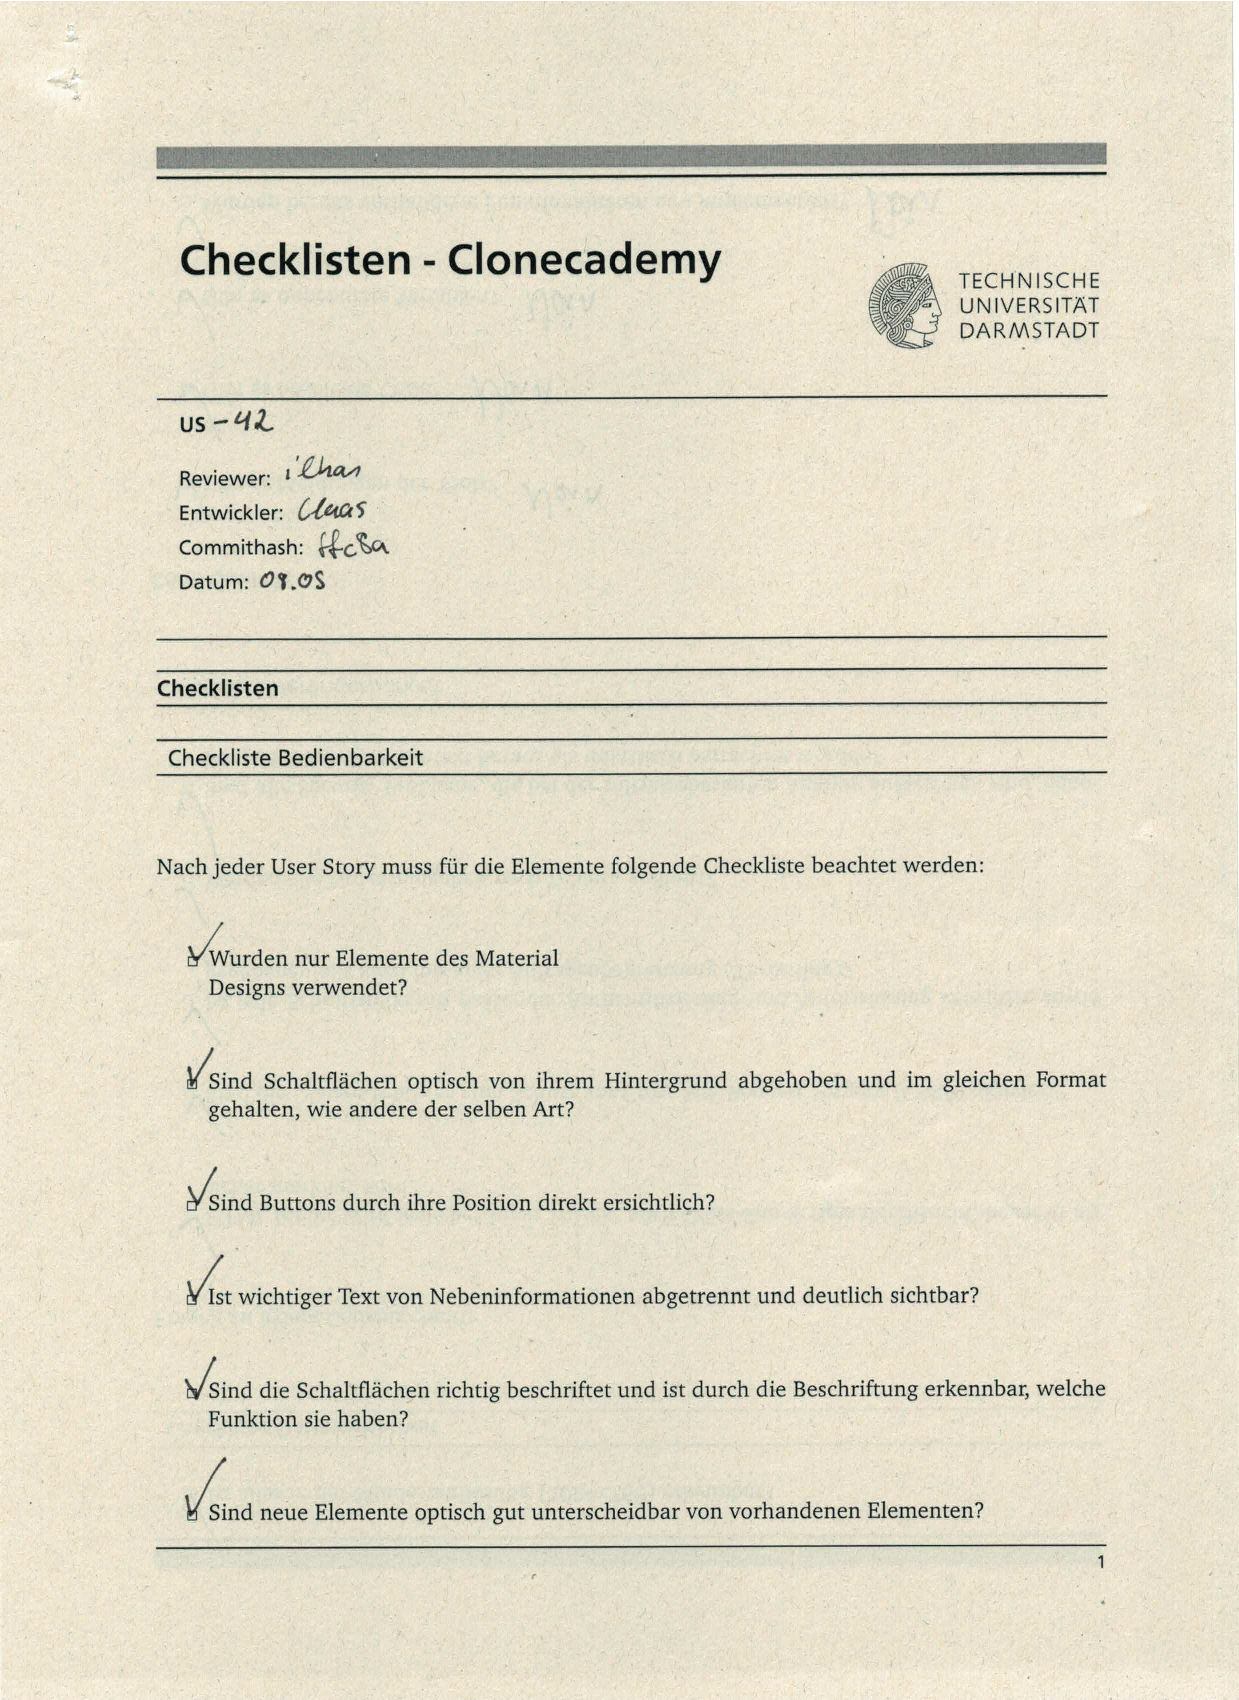
\includepdf[pages=-,pagecommand={},width=\textwidth]{appendix/checklisten/42_01.pdf}
	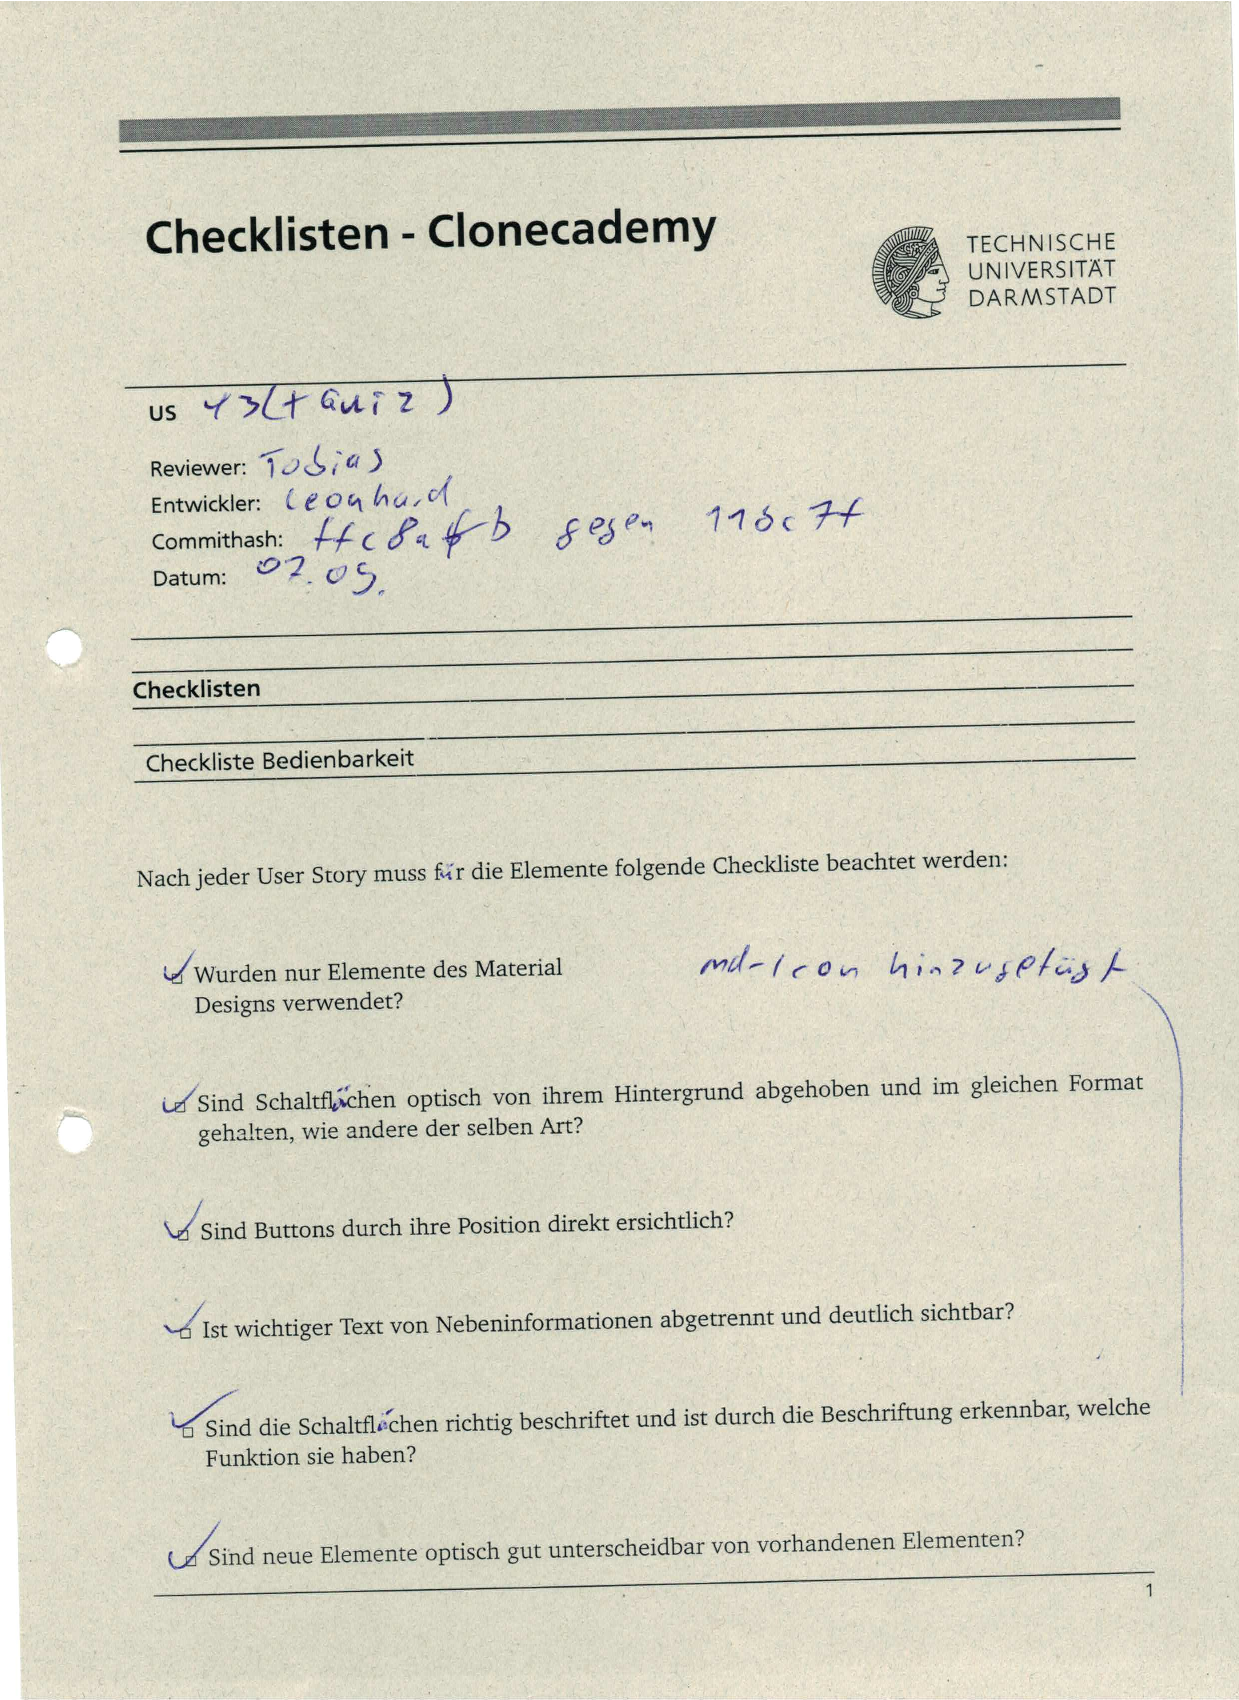
\includepdf[pages=-,pagecommand={},width=\textwidth]{appendix/checklisten/43_01.pdf}
	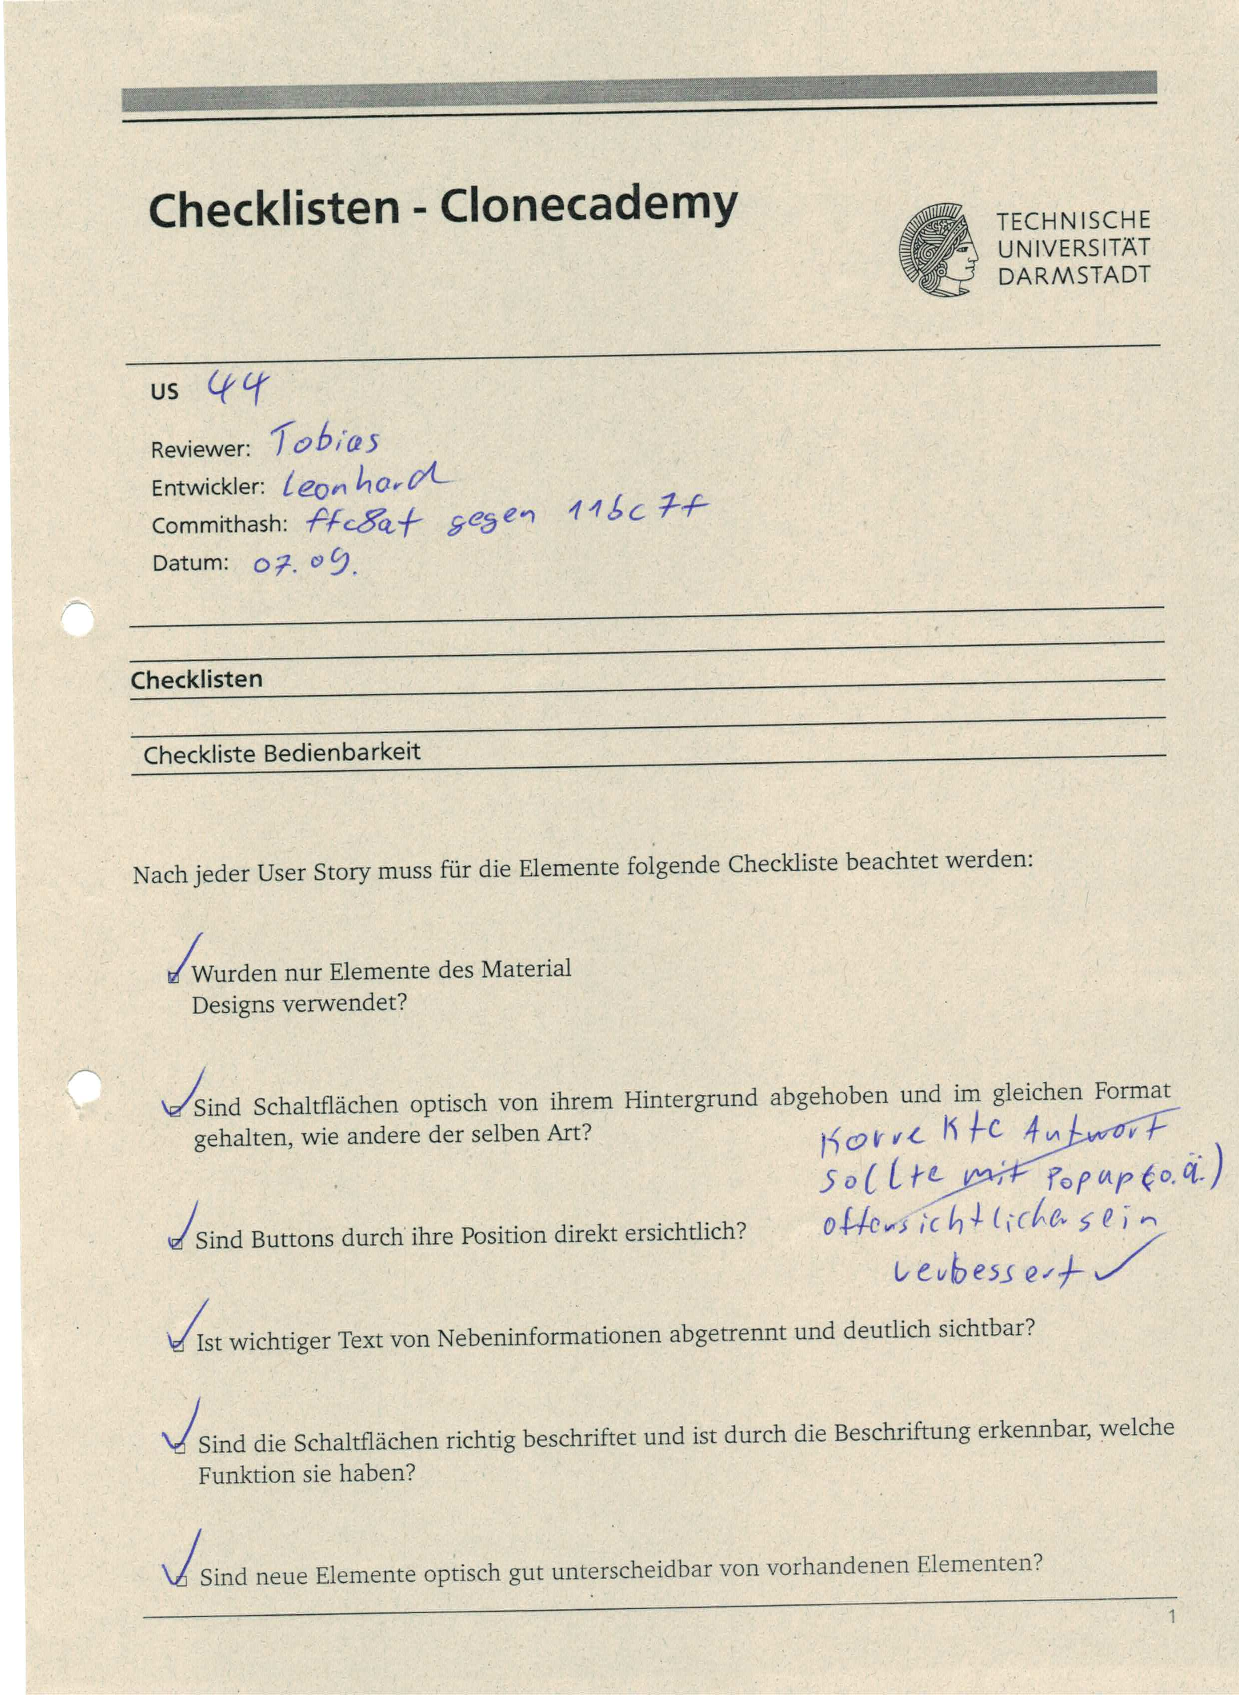
\includepdf[pages=-,pagecommand={},width=\textwidth]{appendix/checklisten/44_01.pdf}
	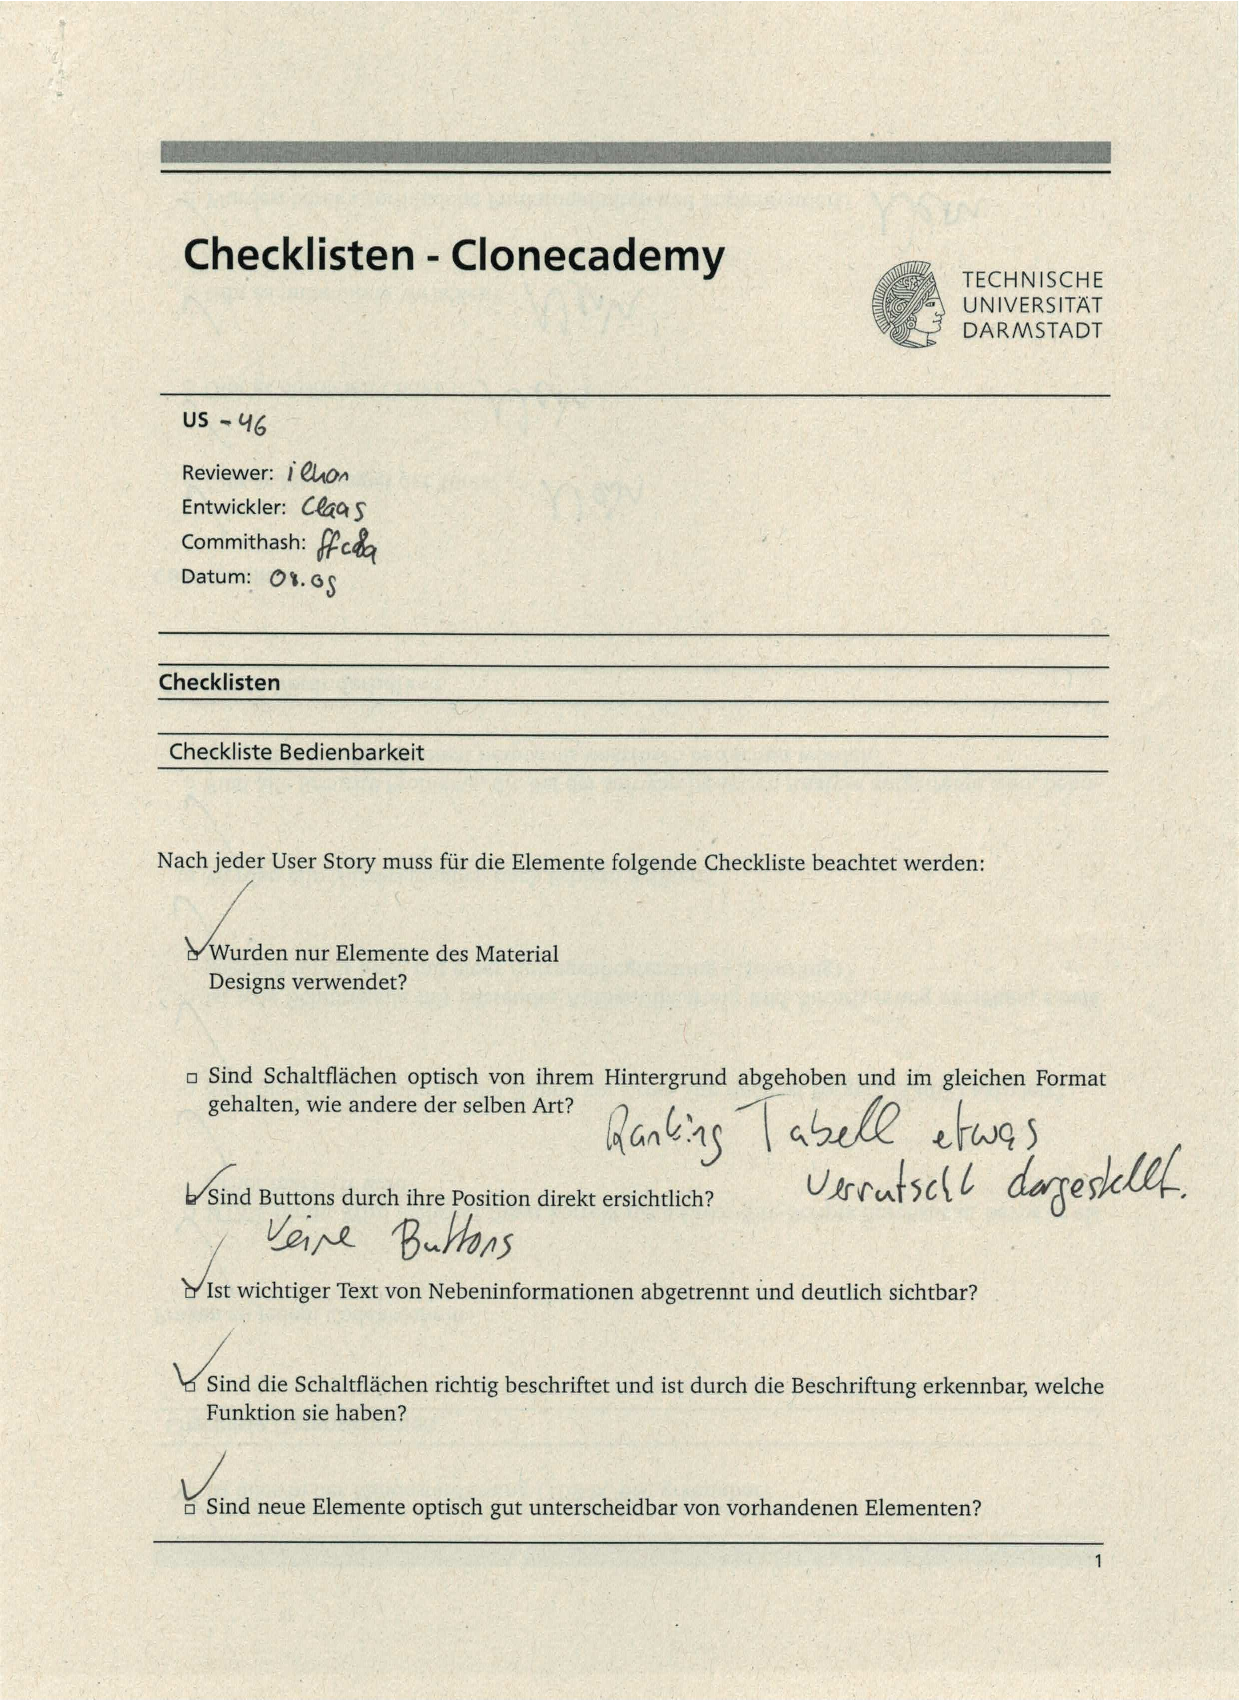
\includepdf[pages=-,pagecommand={},width=\textwidth]{appendix/checklisten/46_01.pdf}

	\subsection*{Veränderbarkeit}
	\subsubsection*{ng lint Output}
	\lstinputlisting{appendix/ng_lint/ng_clean_17.txt}

	\subsubsection*{pylint Output}
	\lstinputlisting{appendix/pylint/meldung_pylint_it17.txt}

	\subsubsection*{coverage Output}
	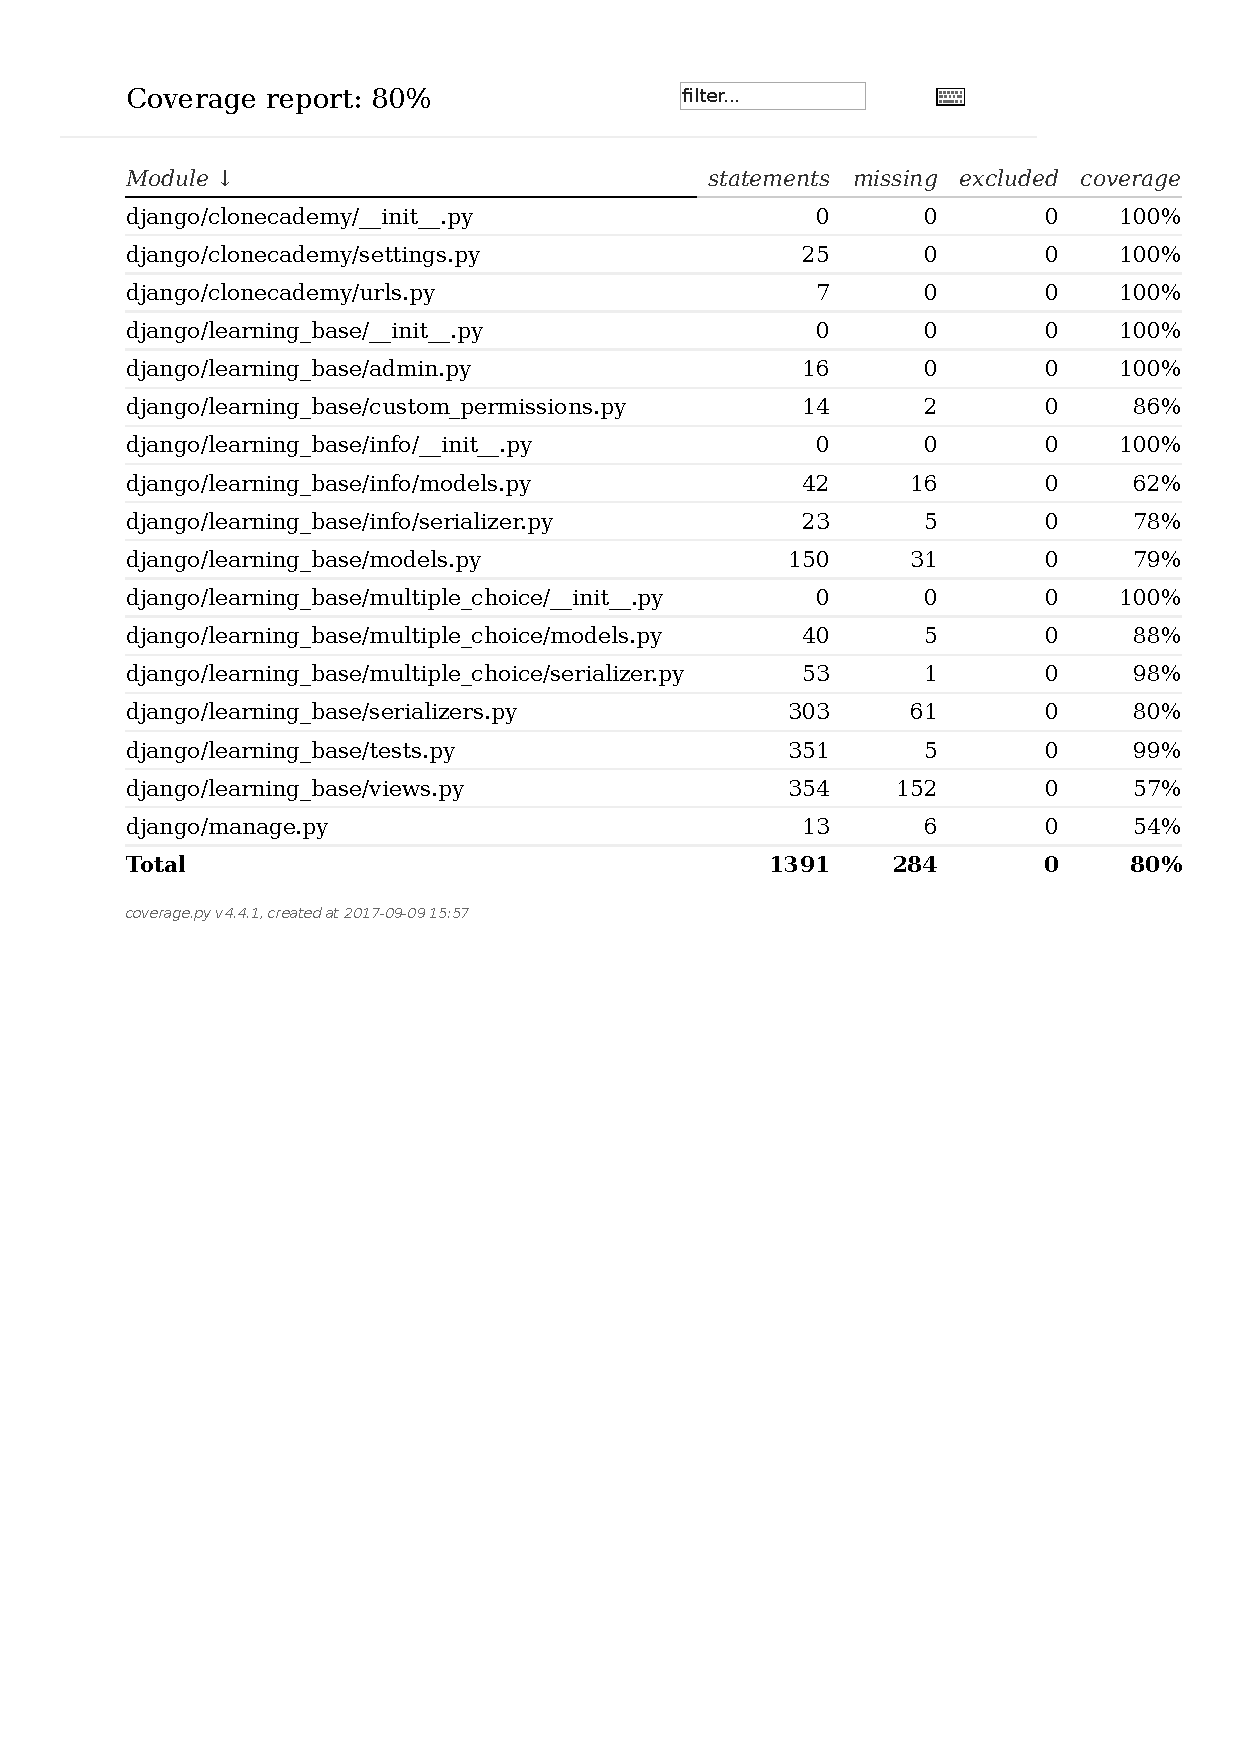
\includepdf[pages=-,pagecommand={},width=\textwidth]{appendix/coverage/django_test_17.pdf}

	\subsection*{Datensicherheit}

	\subsubsection*{bandit Output}
	\lstinputlisting{appendix/bandit/bandit_ffc8a.txt}

\section{Iteration 18 - 14.09.}
	Abgegebene Userstories: 39, 45, 47, 49, 50, 51, 54, 55
	
	Commit Hash: 
	
	\subsection{Checklisten}
	\includepdf[pages=-,pagecommand={},width=\textwidth]{appendix/checklisten/39_01.pdf}
	\includepdf[pages=-,pagecommand={},width=\textwidth]{appendix/checklisten/45_01.pdf}
	\includepdf[pages=-,pagecommand={},width=\textwidth]{appendix/checklisten/47_01.pdf}
	\includepdf[pages=-,pagecommand={},width=\textwidth]{appendix/checklisten/49_01.pdf}
	%\includepdf[pages=-,pagecommand={},width=\textwidth]{appendix/checklisten/50_01.pdf}
	\includepdf[pages=-,pagecommand={},width=\textwidth]{appendix/checklisten/51_01.pdf}
	\includepdf[pages=-,pagecommand={},width=\textwidth]{appendix/checklisten/54_01.pdf}
	\includepdf[pages=-,pagecommand={},width=\textwidth]{appendix/checklisten/55_01.pdf}
	
	\subsection{Veränderbarkeit}
	\subsubsection{ng lint Output}
	\lstinputlisting{appendix/ng_lint/ng_clean_18.txt}

	\subsubsection{pylint Output}
	\lstinputlisting{appendix/pylint/meldung_pylint_it18.txt}

	\subsubsection{coverage Output}
	\includepdf[pages=-,pagecommand={},width=\textwidth]{appendix/coverage/django_test_18.pdf}

	\subsection{Datensicherheit}
	\subsection{bandit Output}
	\lstinputlisting{appendix/bandit/bandit_18.txt}
	

\section*{Iteration 19}
	Abgegebene Userstories: 23, 29, 48, 52, 56, 57, 58
	
	Commit Hash: 
	
	\subsection{Checklisten}
	\includepdf[pages=-,pagecommand={},width=\textwidth]{appendix/checklisten/29_01.pdf}
	\includepdf[pages=-,pagecommand={},width=\textwidth]{appendix/checklisten/29_02.pdf}
	\includepdf[pages=-,pagecommand={},width=\textwidth]{appendix/checklisten/48_01.pdf}
	\includepdf[pages=-,pagecommand={},width=\textwidth]{appendix/checklisten/52_01.pdf}
	\includepdf[pages=-,pagecommand={},width=\textwidth]{appendix/checklisten/56_01.pdf}
	%\includepdf[pages=-,pagecommand={},width=\textwidth]{appendix/checklisten/57_01.pdf}

	\subsection*{Veränderbarkeit}
	\subsubsection*{ng lint Output}
	\lstinputlisting{appendix/ng_lint/ng_clean_19.txt}

	\subsubsection*{pylint Output}
	\lstinputlisting{appendix/pylint/meldung_pylint_it19.txt}

	\subsubsection*{coverage Output}
	\includepdf[pages=-,pagecommand={},width=\textwidth]{appendix/coverage/django_test_19.pdf}

	\subsection*{Datensicherheit}

	\subsubsection*{bandit Output}
	\lstinputlisting{appendix/bandit/bandit_18.txt}

	
\section*{Release 1 - 07.08.2017}
Späteste Durchführung aller Tests: 30.07.2017

Commit Hash der Serverversion (master branch): 

\subsection*{Nutzerstudie - Protokoll}
\includepdf[pages=-,pagecommand={},width=\textwidth]{../nutzerstudien/protokoll-06_28_2017.pdf}

\subsection*{Nutzerstudie - Fragebögen}


\subsection*{Zed Attack Proxy Tool - Diskussion}
Alle gefundenen Fehler betreffen nur die Konfiguration des Servers, nicht das Produkt an sich. Da wir im Gespräch mit den Auftraggeber*innen vereinbart hatten, dass wir nicht dafür zuständig sind, den Server zu sichern, ist das Korrigieren diese Fehler nicht Teil unserer Aufgabe.

Dennoch wollen wir für die kommenden Releases Empfehlungen geben, wie diese Probleme verhindert werden können. Claas recherchiert dazu zu den einzelnen Fehlern und schreibt eine kurze Anleitung, wie die richtigen Einstellung lauten. Diese werden dann an die Auftraggeber*innen weiter gegeben.

\subsection*{Zed Attack Proxy Tool - Output}
\includepdf[pages=-,pagecommand={},width=\textwidth]{appendix/zap/zap_pre_release_august.pdf}


\section*{Release 2 - 13.09.2017}
Durchführung aller Tests: 06.09.2017

Commit Hash der Serverversion (master branch): 

\subsection*{Nutzerstudie - Protokoll}
\includepdf[pages=-,pagecommand={},width=\textwidth]{../nutzerstudien/protokoll-09_06_2017.pdf}

\subsection*{Nutzerstudie - Fragebögen}


\subsection*{Zed Attack Proxy Tool - Diskussion}
Der in der letzten Iteration gefundene Fehler mit einer Gefährlichkeit von ''Medium'' wurde inzwischen behoben. Die verbleibenden Fehler wurden bislang nicht bearbeitet. Claas hat die notwendigen Daten allerdings an die Auftraggeber*innen geschrieben.

Wir empfehlen erneut, die Serverkonfiguration zu ändern.

Anhängend ein Auszug aus der beispielhaften Server-Konfiguration:

\lstinputlisting{appendix/code_documentation/nginx-app.conf}

\subsection*{Zed Attack Proxy Tool - Output}
\includepdf[pages=-,pagecommand={},width=\textwidth]{appendix/zap/zap_pre_release_september.pdf}


\section*{Release 3 - 01.10.2017}
Durchführung aller Tests: 22.09.2017

Commit Hash der Serverversion (master branch): 

\subsection*{Nutzerstudie - Protokoll}
\includepdf[pages=-,pagecommand={},width=\textwidth]{../nutzerstudien/protokoll-09_25_2017.pdf}

\subsection*{Nutzerstudie - Fragebögen}

\chapter*{Progression des Design}

\section*{Planungsphase}
Dies war der ursprüngliche Plan für das Layout der Seite. Dieses Design wurde mit den Auftraggeber*innen erarbeitet.

\includepdf[pages=-,pagecommand={},width=\textwidth]{../BeispielDesign/Dashboard.pdf}
\includepdf[pages=-,pagecommand={},width=\textwidth]{../BeispielDesign/MultipleChoice.pdf}

\section*{Minimum Viable Product}
Im folgenden ist ein Screenshot vom Frontend gezeigt, nachdem die Webseite funktional war.

\includegraphics[width=\textwidth]{appendix/screenshots/forntend.png}

\section*{Abgabefertiges Produkt}
Im folgenden ist der Stand des Produktes bei Abgabe zu sehen.

\includegraphics[height=0.3\textheight]{appendix/screenshots/dashboard.jpg}

\includegraphics[height=0.3\textheight]{appendix/screenshots/screenshot-0.jpg}

\includegraphics[height=0.3\textheight]{appendix/screenshots/question-0.jpeg}



\chapter*{Dokumentation des Codes - Auszüge}

Wir haben uns dafür entschieden, jeweils drei Klassen us dem Front- und dem Backend vorzuweisen. Dies liegt daran, dass wir die Komponenten separat entwickelt haben und die Qualität in beiden Teilen des Projektes wichtig für die weitere Verwendbarkeit ist.

\section*{Course Service - Frontend}
Der Course Service ist der zentrale Dreh- und Angelpunkt über den das Frontend die Lerndaten vom Backend anfragt.

\lstinputlisting[language=Java]{appendix/code_documentation/course.service.ts}

\section*{User Details - Frontend}
User Details ist eine komplexe Klasse, die es ermöglicht, Einstellungen zu verändern. Sie zeigt gut, wie der Code des Frontends aufgebaut ist.

\lstinputlisting[language=Java]{appendix/code_documentation/user-detail.component.ts }

\section*{Statistics - Frontend}
Statistics zeigt den Nutzer*innen ihre Nutzungsstatistiken auf der Plattform an. 

\lstinputlisting[language=Java]{appendix/code_documentation/statistics.component.ts }

\section*{Course object - Backend}
Das Course Objekt repräsentiert den betreffenden Eintrag in der Datenbank und stellt weitere Funktionalitäten für das Backend bereit.

\lstinputlisting[language=Java]{appendix/code_documentation/course.py }

\section*{Question object - Backend} 

\lstinputlisting[language=Java]{appendix/code_documentation/question.py }

\section*{CourseView object - Backend}
Die Klasse CourseView modelliert die REST-Schnittstelle über die auf Kurse zugegriffen werden kann.

\lstinputlisting[language=Java]{appendix/code_documentation/course_view.py }

\chapter{Unittests}

Dies sind die Testklassen bei Stand der Abgabe

\section{Python Tests}
\lstinputlisting[language=Python]{appendix/tests.py}

\section{Protractor/Selenium Tests}
\lstinputlisting[language=Java]{appendix/specs.js}

\chapter{Abschließende Coverage}
Hier angefügt ist ein vollständiger Coverage-Report.

\includepdf[pages=-,pagecommand={},width=\textwidth]{appendix/coverage/django_test_19.pdf}
\includepdf[pages=-,pagecommand={},width=\textwidth]{appendix/coverage/django_learning_base_info_models.pdf}
\includepdf[pages=-,pagecommand={},width=\textwidth]{appendix/coverage/django_learning_base_info_serializer.pdf}
\includepdf[pages=-,pagecommand={},width=\textwidth]{appendix/coverage/django_learning_base_models.pdf}
\includepdf[pages=-,pagecommand={},width=\textwidth]{appendix/coverage/django_learning_base_multiple_choice_models.pdf}
\includepdf[pages=-,pagecommand={},width=\textwidth]{appendix/coverage/django_learning_base_multiple_choice_serializer.pdf}
\includepdf[pages=-,pagecommand={},width=\textwidth]{appendix/coverage/django_learning_base_views.pdf}


\chapter{GitHub-Wiki}
Das Team hat die Dokumentation der REST-API wie geplant im GitHub Wiki des Repositories geführt. Um die Webseiten lesbar für dieses Dokument zu machen, haben wir die Markdown Seiten der WIki in \LaTeX Code umgewandelt. Im folgenden sind die einzelnen Seiten aufgeführt.

\chapter*{UserView}

\section*{Introduction}\label{introduction}

The UserView class is used to view information about a single user. The
`post' method is used to register new users

The request can be accessed via ``clonecademy/user/''

The url ``clonecademy/user/'' Points to the user itself.

\section*{Method Details}\label{method-details}

\subsection*{\texorpdfstring{`get'}{get}}\label{get}

Permissions: mod or higher for other, user for self

Header: user id (for permissions)

Response:

\begin{verbatim}
{
"id": number id,
"username": sting "The users username",
"email": string "the users email address",
"first_name": string "First name of the user (if provided, else empty)",
"last_name": string "First name of the user (if provided, else empty)",
"groups": [string] "A array of strings with the names of the group. E.g ['moderator', 'admin'],
"date_joined": string "The date on which this user was created",
"language": string "short form of the language, 'eg' for english"
"avatar": string "encoded image of this user",
"ranking": number "the ranking of the current user"
}
\end{verbatim}

\subsection*{\texorpdfstring{`post'}{post}}\label{post}

Header:

Request:

\begin{verbatim}
{
  "user_id": number id;
  "username": string "The users username";
  "email": string "the users email address";
  "password": string "the chosen password of the user";
  ("first_name": string "First name of the user";)
  ("last_name": string "First name of the user";)
  ("age": string "birthday of the user")
}
\end{verbatim}

Response: 200 (user saved), 500 + serializer error (error)

 \chapter*{Course View}

\section*{Introduction}\label{introduction}

The CourseView class is used to get information for a specific course.
Courses are referenced via the general url ``clonecademy.com/courses/''.

\section*{Method Details}\label{method-details}

\subsection*{\texorpdfstring{`get'}{get}}\label{get}

Header: user id (for permissions), course id (from url)

Response:

\begin{verbatim}
{
"name": string "Course name";
"difficulty": number 0/1/2/3;
"category": string "iGEM/General";
"language": string "de/en";
"modules": [{
              "name": string "Module name";
              "learning_text": string "Sample learning text";
              "questions": [{
                              "type": string "MultipleChoiceQuestion";
                              "solved": boolean True/False;
                            }];
            }];
}
\end{verbatim}

\subsection*{\texorpdfstring{`post'}{post}}\label{post}

Header: user id (for permissions)

Request:

\begin{verbatim}
{
"name": string "Course name",
"difficulty": number 0/1/2/3,
"modules": [{
              "name": string "Module name",
              "learning_text": string "Sample learning text";
              "questions": [{
                              "type": string "MultipleChoiceQuestion";
                              "question_title": string "(currently blank)";
                              "question_body": string "The text for the question";
                              "feedback": string "A specific feedback text (leave empty for standard)"
                            }]
            }]
"quiz": [{
        "question" : string,
        "image": string,
        "answers": [{
                    "text": string,
                    "img": string,
                    "correct": boolean,
                    }]
         }]
}
\end{verbatim}

Response: 201 (saved), 500 + serializer error (error)
\chapter*{GrantModRightsView}

\section*{Introduction}\label{introduction}

The GrantModRightsView class is used to promote a user to a moderator by adding him*her to the usergroup 'moderator'. It also provides a get method to check whether a user is already part of the group.

\section*{Method Details}\label{method-details}

\subsection*{\texorpdfstring{`get'}{get}}\label{get}

URL: user\_id

Returns true, iff the user in the url is a moderator

Request

Response

\begin{verbatim}
True|False (200)
\end{verbatim}

\subsection*{\texorpdfstring{`post'}{post}}\label{post}

Header: user\_id Request:

\begin{verbatim}
{ }
\end{verbatim}

Note: can be used for other permissions in the future

Response:

\begin{verbatim}
"successfully promoted " + to_be_promoted.username (200)
"the user \" "+ to_be_promoted.username +"\" is already a moderator" (200)
\end{verbatim}

\chapter*{MultiCourseView}

\section*{Introduction}\label{introduction}

The MultiCourseView class is used to get information for all courses. The
course list can be accessed by calling ``clonecademy/courses/list''

\section*{Method Details}\label{method-details}

\subsection*{\texorpdfstring{`get'}{get}}\label{get}

Not implemented, due to the need for further filtering

\subsection*{\texorpdfstring{`post'}{post}}\label{post}

Header: user id (for permissions)

Request:

\begin{verbatim}
{
"type": string "all/mod/started"
"category": string "iGEM/General/all"
"language": string "de/en"
}
\end{verbatim}

Response:

\begin{verbatim}
[{
"id": string "the courses id",
"name": string "the courses name",
"category": string "iGEM/...",
"num_questions": int "amount of questions in the course",
"num_answered": int "amount of questions the user answered",
"responsible_mod": int "the id of the responsive moderator for this course",
}]
\end{verbatim}

\chapter*{MultiUserView}

\section*{Introduction}\label{introduction}

The MultiUserView class is used to show information about all users.

The request can be accessed via ``clonecademy/user/all''

\section*{Method Details}\label{method-details}

\subsection*{\texorpdfstring{`get'}{get}}\label{get}

Permissions: mod or higher

Header: user id (for permissions)

Response: {[}\{ ``user\_id'': ``id''; ``username'': ``The users
username''; \}{]}

\subsection*{\texorpdfstring{`post'}{post}}\label{post}

Not implemented yet (could be used for filtering the input list)

\chapter*{QuestionView}

\section*{Introduction}\label{introduction}

The QuestionView class provides information about every
question, provided the user is allowed to see the question. The class is
also used to answer questions.

\section*{Method Detais}\label{method-detais}

\subsection*{\texorpdfstring{`get'}{get}}\label{get}

Header: user id (for permissions), course id (from url), ordered
position of module in coures (from url), ordered position of question in
module (from url)

Response:

\begin{verbatim}
{
"title": string "Question title (currently from module)"
"body": string "Question text"
"feedback": string "Feedback for user after correct answer"
"last": boolean "True/False"
"module": string "the corresponding module for the question"
"last_module": boolean "True/False"
"learning_text": string "The modules learning text"
"course": string "the corresponding course"
"progress": [[string]] "contains the title of all questions of this course"
}
\end{verbatim}

Error:

Response: 400 if unauthorized // only allowed for user if it is the
first in this course or if the user answered the questions before
correct

\subsection*{\texorpdfstring{`post'}{post}}\label{post}

Header: user id (for permissions), course id (from url), ordered
position of module in coures (from url), ordered position of question in
module (from url)

Request:

\begin{verbatim}
{
"answers":depends on the question type 
}
\end{verbatim}

Response:

\begin{verbatim}
{
"solved": boolean true/false;
"next": string "question/module/quiz for the next element"
}
\end{verbatim}

Response: 200 (correct answer, try saved), 400 unauthorized, 500+
serializer error

Error:

Response: 400 if unauthorized // only allowed for user if it is the
first in this course or if the user answered the questions before
correct

\chapter*{QuizView}

\section*{Introduction}\label{introduction}

The QuizView class provides information about every quiz
question, provided the user is allowed to see the quiz question. The
class is also used to answer quiz questions.

\section*{Method Detais}\label{method-detais}

\subsection*{\texorpdfstring{`get'}{get}}\label{get}

Header: user id (for permissions), course id (from url), ordered
position of module in coures (from url), ordered position of question in
module (from url)

Response:

\begin{verbatim}
{
"id": number,
"question": string,
"imgage": string,
"answers": [{
           "id": number,
           "text": string,
           "img": string
           }]
}
\end{verbatim}

Error:

Response: 400 if unauthorized // only allowed for user if it is the
first in this course or if the user answered the questions before
correct

\subsection*{\texorpdfstring{`post'}{post}}\label{post}

Header: user id (for permissions), course id (from url)

Request:

\begin{verbatim}
[{
 "id": number "the quiz question id"
 "answers": [{
            "chosen": boolean "if true the user has checked this quiz question"
            "id": number "the id of the quiz answer"
            }]
}]
\end{verbatim}

Response:

\begin{verbatim}
[{
"name": string "the title of the quiz question",
"solved": boolean "if the answer was correct"
}]
\end{verbatim}

Response: 200 (correct answer, try saved), 400 unauthorized, 500+
serializer error

Error:

Response: 400 if unauthorized // only allowed for user if it is the
first in this course or if the user answered the questions before this one
correctly


\chapter*{RequestView}

\section*{Introduction}\label{introduction}

The RequestView class is used to submit a request for moderator rights.

The request can be accessed via ``clonecademy/user/request/''

\section*{Method Details}\label{method-details}

\subsection*{\texorpdfstring{`get'}{get}}\label{get}

Header: user id (for permissions and filtering)

Response: 200 (can submit request), 403 + reason (is mod or too many mod
requests)

\subsection*{\texorpdfstring{`post'}{post}}\label{post}

Header: user id (for permissions and saving)

Request:

\begin{verbatim}
{
"reason": string "the reason for the request",
}
\end{verbatim}

Response: 200 (request sent), 500 + serializer error (error)

Side effects: sends an email to the admins requesting mod access


\chapter*{StaticPages}

\section*{Static pages}

All static pages are html Pages and have to be in the folder
\textbf{assets/statics} To find the Page on the menu you have to add it
in the \textbf{menu.componenent.ts} in the variable \textbf{links}.

\texttt{\{\ url:\ (string)\ has\ to\ be\ the\ name\ of\ the\ file\ without\ html,\ name:\ (string)\ will\ be\ the\ name\ in\ the\ dropdown\ menu\ \}}

The order of the objects in the link variable is the order of the
dropdown menu.


\chapter*{StatisticsView}

\section*{Introduction}\label{introduction}

The StatisticsView class is used to get information about the usage
statistics. The get method returns all Try objects, detailing all
questions and the respective answers, the post method saves a new Try
object, when an answer is submitted.

Statistics can be accessed via ``clonecademy/statistics/''

\section*{Method Details}\label{method-details}

\subsection*{\texorpdfstring{`get'}{get}}\label{get}

Header: user id (for permissions and filtering)

Response:

\begin{verbatim}
[{
"question": string "the questions id";
"module": string "The questions module"
"course": string "The questions course"
"solved": boolean True/False;
"date": string "The date of the try"
}]
\end{verbatim}

\subsection*{\texorpdfstring{`post'}{post}}\label{post}

Header: user id (for permissions and filtering)

Post:

\begin{verbatim}
{ 
 "format": string "valid formats are 'csv' or empty for json";
 "id": string "the user ID if the user is not a moderator or a admin this must be set;
 "get_courses": any "if this field is set and the current user is a moderator or admin it will return all courses of which it created;
"course": number "get the statistics for this course (with prefiltering admin moderator id);
"date": {
          "start": string "the start date for the statistics it has to be the format '%Y-%m-%d %H:%M:%S'";
          "end": string "the end date for the statistics '%Y-%m-%d %H:%M:%S'";
        },
"serialize": string "get more fields of the statistics for example question__module__course__id returns a field with the course id"
"order": string "order the tries",
"filter": string "filter the statistics for this class and count the amounts"
}
\end{verbatim}

Response:

\begin{verbatim}
[{
"question": string "the questions id";
"user": string "The User for this try";
"solved": boolean True/False;
"date": string "The date of the try"
}]
\end{verbatim}



\chapter*{ToggleCourseVisibilityView}

\section*{Introduction}\label{introduction}

This class is used to change the ``is\_visible'' state of a course.
`True' means, that users can see the course in their dashboards and
False the opposite. Courses are referenced via the general url
``clonecademy.com/courses/''.

\section*{Method Details}\label{method-details}

\subsection*{\texorpdfstring{`post'}{post}}\label{post}

Header: user id (for permissions), course id (from url)

Request: Leaving out the ``is\_visible'' content of the request, and
therefore posting no data at all, toggles the state.

\begin{verbatim}
{
"is_visible": True|False (optional)  
}
\end{verbatim}

Response: 200 (visibility changed), 400-404 (Bad Requests), 500+
(internal error)

\chapter*{UserRightsView}

\section*{Introduction}\label{introduction}

The UserRightsView class is used to promote or demote a user to
Moderator or Admin.

\section*{Method Details}\label{method-details}

\subsection*{\texorpdfstring{`get'}{get}}\label{get}

No get Method implemented

\subsection*{\texorpdfstring{`post'}{post}}\label{post}

Header: user\_id Request:

\begin{verbatim}
{
'right': string "the group in which the user will be pro or demoted",
'action': string "promote or demote",
}
\end{verbatim}

Response:

The response is identical to the UserView get method


\chapter*{UserView}

\section*{Introduction}\label{introduction}

The UserView class is used to view information about a single user. The
`post' method is used to register new users

The request can be accessed via ``clonecademy/user/''

The url ``clonecademy/user/'' Points to the user itself.

\section*{Method Details}\label{method-details}

\subsection*{\texorpdfstring{`get'}{get}}\label{get}

Permissions: mod or higher for other, user for self

Header: user id (for permissions)

Response:

\begin{verbatim}
{
"id": number id,
"username": sting "The users username",
"email": string "the users email address",
"first_name": string "First name of the user (if provided, else empty)",
"last_name": string "First name of the user (if provided, else empty)",
"groups": [string] "A array of strings with the names of the group. E.g ['moderator', 'admin'],
"date_joined": string "The date on which this user was created",
"language": string "short form of the language, 'eg' for english"
"avatar": string "encoded image of this user",
"ranking": number "the ranking of the current user"
}
\end{verbatim}

\subsection*{\texorpdfstring{`post'}{post}}\label{post}

Header:

Request:

\begin{verbatim}
{
  "user_id": number id;
  "username": string "The users username";
  "email": string "the users email address";
  "password": string "the chosen password of the user";
  ("first_name": string "First name of the user";)
  ("last_name": string "First name of the user";)
  ("age": string "birthday of the user")
}
\end{verbatim}

Response: 200 (user saved), 500 + serializer error (error)
	


\chapter{Userstories}
\documentclass
[english,accentcolor=tud1c]
{tudreport}

\usepackage[T1]{fontenc}
\usepackage[utf8]{inputenc}
\usepackage{amstext}
\usepackage{amsmath}
\usepackage{graphicx}
\usepackage{setspace}
\usepackage{multicol}
\usepackage{mathtools}
\usepackage{dsfont}
\usepackage{units}
\usepackage{subfigure}
\usepackage{color}
\usepackage{booktabs}
\usepackage{fancyref}
\usepackage[ngerman,english]{babel}
\usepackage{pdfpages}
\usepackage{tabularx}

\title{User Stories\\Clonecademy}
\author{Tobias Huber, Leon Wiedmann, Ilhan , Claas Alexander Voelcker}


\begin{document}

	%=========================================================

	\maketitle

	\chapter{Iteration}
	In dieser Iteration wurden grundlegende Dinge besprochen und die benötigten Frameworks aufgesetzt.

	Es konnten noch keine Userstories umgesetzt werden. 

	\chapter{Iteration}

	\begin{tabularx}{\textwidth}{|p{.2\textwidth}|X|}
	\hline
	ID & 2\\
	\hline
	Benutzerrolle & Nutzer\\
	\hline
	Name & Authentifizierung\\
	\hline
	Beschreibung & Als Nutzer möchte ich mich auf der Seite als Nutzer einloggen können.\\
	\hline
	Akzeptanzkriterium & Das Authentifizerungsfenster wird korrekt angezeigt. Bei gültiger Eingabe seiner Daten wird der Nutzer auf die Kursübersicht weitergeleitet und ein Authetifizierungstoken wird generiert, der zur Authetifizierung weitergereicht wird. Bei ungültiger Eingabe wird der Nutzer durch ein Popup darauf hingewiesen und nicht eingelogt.\\
	\hline
	Story Points & 2 \\
	\hline
	Entwickler & Leonhard Wiedmann\\
	\hline
	Umgesetzt in Iteration & 1\\
	\hline
	Tatsächlicher Aufwand & 3.5 h\\
	\hline
	Velocity & 1.75 h/SP\\
	\hline
	Bemerkung & \\
	\hline
\end{tabularx}
\vspace{20pt}
 \\
	\begin{tabularx}{\textwidth}{|p{.2\textwidth}|X|}
	\hline
	ID & 3\\
	\hline
	Benutzerrolle & Moderator*in\\
	\hline
	Name & Neuen Kurs anlegen\\
	\hline
	Beschreibung & Als Moderator*in möchte ich einen neuen Kurs anlege können. Dazu gehe ich auf die Kursübersicht und wähle die Schaltfläche ''Add Course'' aus. Ein Editor erlaubt mir, Name und Kategorie des Kurses auszuwählen. Danach kann ich den Kurs speichern und er taucht auf der Übersichtsseite auf. Der Kurs ist erste einmal nur für Moderator*innen sichtbar.
\\
	\hline
	Akzeptanzkriterium & Der neu angelegte Kurs mit Name und Kategorie wird persistent gespeichert und ist für Moderator*innen einsehbar.\\
	\hline
	Story Points & 3\\
	\hline
	Entwickler & Claas Völcker \& Leonhard Wiedmann\\
	\hline
	Umgesetzt in Iteration & 1\\
	\hline
	Tatsächlicher Aufwand & 3 h\\
	\hline
	Velocity & 1.5 h/SP\\
	\hline
	Bemerkung & Die genaue Funktionsweise des Editors wurde in einem Gespräch mit den Auftraggeber*innen festgelegt.\\
	\hline
\end{tabularx}
\vspace{20pt}



	\chapter{Iteration}

	\begin{tabularx}{\textwidth}{|p{.2\textwidth}|X|}
	\hline
	ID & 5\\
	\hline
	Benutzerrolle & Nutzer*in\\
	\hline
	Name & Kurs auswählen\\
	\hline
	Beschreibung & Als Nutzer*in möchte ich aus einer Kursübersicht einen Kurs auswählen und im Folgenden die Fragen des Kurses beantworten können. Nachdem ich den Kurs ausgewählt habe, soll er in meiner persönlichen Kursübersicht samt Fortschrittsangabe angezeigt werden.\\
	\hline
	Akzeptanzkriterium & Der ausgewählte Kurs wird vollständig angezeigt und die Fragen können bearbeitet und zugleich jederzeit abgebrochen werden.Der Fortschritt wird gespeichert und in einer persönlichen Statistik angezeigt. Nach Abbrechen einer Frage kann die Bearbeitung derselben jederzeit fortgesetzt werden.\\
	\hline
	Story Points & 7\\
	\hline
	Entwickler & Ilhan Simsiki\\
	\hline
	Umgesetzt in Iteration & 3\\
	\hline
	Tatsächlicher Aufwand & 11 h\\
	\hline
	Velocity & 1.57 h/SP\\
	\hline
	Bemerkung & \\
	\hline
\end{tabularx}
\vspace{20pt}
 \\
	\begin{tabularx}{\textwidth}{|p{.2\textwidth}|X|}
		\hline
		ID & 1 \\
		\hline
		Benutzerrolle & Nutzer \\
		\hline
		Name & Nutzer erstellen \\
		\hline
		Beschreibung & Als Nutzer möchte ich auf der Seite einen eigenen Account anlegen können. Mit Ausfüllen des Anmeldeformulars mit den Pflichtfeldern:
		E-Mail-Adresse,
		Benutzername,
		Passwort.
		Und den Optionalen Feldern:
		Vorname,
		Nachname,
		Alter \\
		\hline
		Akzeptanzkriterium & Das Anmeldeformular wird korrekt dargestellt. Mit dem Klicken des ''Registrieren'' Buttons und Ausfüllen der Pflichtfelder wird der Account persistent in der Datenbank gespeichert. \\
		\hline
		Story Points & 2 \\
		\hline
		Entwickler & Tobias Huber \\
		\hline
		Umgesetzt in Iteration & \\ 
		\hline
		Tatsächlicher Aufwand &  \\
		\hline
		Velocity &  \\
		\hline
		Bemerkung &  \\
		\hline
\end{tabularx}
\vspace{20pt}
 \\
	\begin{tabularx}{\textwidth}{|p{.2\textwidth}|X|}
	\hline
	ID & 8\\
	\hline
	Benutzerrolle & Nutzer*in\\
	\hline
	Name & Frage beantworten\\
	\hline
	Beschreibung & Ein*e Nutzer*in möchte eine Frage beantworten. Dabei wird jede Frage ausgewertet, und dem*der Nutzer*in wird angezeigt, ob die Eingabe richtig oder falsch war. War die Beantwortung korrekt, wird die nächste Frage angezeigt.\\
	\hline
	Akzeptanzkriterium & Die Frage kann beantwortet werden und das Ergebnis wird in der Datenbank unter Statistik gespeichert.\\
	\hline
	Story Points & 7 Story Points\\
	\hline
	Entwickler & Leonhard Wiedmann\\
	\hline
	Umgesetzt in Iteration & 4\\
	\hline
	Tatsächlicher Aufwand & 14 h\\
	\hline
	Velocity & 2 h/SP\\
	\hline
	Bemerkung & Es werden neue Daten in die Datenbank geschrieben.\\
	\hline
\end{tabularx}
\vspace{20pt}



	\chapter{Iteration}

	\begin{tabularx}{\textwidth}{|p{.2\textwidth}|X|}
	\hline
	ID & 6\\
	\hline
	Benutzerrolle & Nutzer\\
	\hline
	Name & Statistik einsehen\\
	\hline
	Beschreibung & Als Nutzer möchte ich einen Button ''Meine Statistik'' anklicken können. Nach Anklicken erscheint eine Seite, auf der ich meine bisherigen beantworteten Fragen sehen kann: Wie viele Fragen habe ich richtig beantwortet, wie viele sind falsch.\\
	\hline
	Akzeptanzkriterium & Die Statistik des Nutzers wird nach Klicken auf die dafür vorgesehene Schaltfläche vollständig angezeigt.\\
	\hline
	Story Points & 8 Story Points\\
	\hline
	Entwickler & Claas Völcker\\
	\hline
	Umgesetzt in Iteration & 4\\
	\hline
	Tatsächlicher Aufwand & 8 h\\
	\hline
	Velocity & 1 h/SP\\
	\hline
	Bemerkung &  Es werden keine Daten in der Datenbank geändert.\\
	\hline
\end{tabularx}
\vspace{20pt}
 \\
	\begin{tabularx}{\textwidth}{|p{.2\textwidth}|X|}
	\hline
	ID & 7\\
	\hline
	Benutzerrolle & Moderator\\
	\hline
	Name & Multiple Choice Fragen einpflegen\\
	\hline
	Beschreibung & Als Moderator kann ich einem Kurs neue Fragen hinzufügen. Dazu wähle ich auf der Kursübersicht die Schaltfläche neue Frage anlegen aus. Ich kann daraufhin in einem Interface den Name der Frage, den Text der Frage und mögliche Antwortmöglichkeiten eingeben. In einem weiteren Fenster kann ich einen Text eingeben, der den Nutzenden bei erfolgreicher Bearbeitung angezeigt wird und einen Feedbacktext bei falscher Beantwortung.\\
	\hline
	Akzeptanzkriterium & Eine neu angelegte Frage wird persistent unter dem Kurs gespeichert und ist nach Freigabe für Nutzende bearbeitbar.\\
	\hline
	Story Points & 8 Story Points\\
	\hline
	Entwickler & Leonhard Wiedmann\\
	\hline
	Umgesetzt in Iteration & 4\\
	\hline
	Tatsächlicher Aufwand & 15 h\\
	\hline
	Velocity & 1.875 h/SP\\
	\hline
	Bemerkung & Moderatoren können nur Fragen in ihren eigenen Kursen anlegen. Es werden neue Daten in die Datenbank geschrieben, aber keine existierenden verändert oder gelöscht.\\
	\hline
\end{tabularx}
\vspace{20pt}



	\chapter{Iteration}

	\begin{tabularx}{\textwidth}{|p{.2\textwidth}|X|}
	\hline
	ID & 9\\
	\hline
	Benutzerrolle & Admin\\
	\hline
	Name & Nutzerliste einsehen\\
	\hline
	Beschreibung & Als Admin möchte ich mir eine Übersicht über die vorhandenen Nutzer*innen anzeigen lassen und für alle eine Detailansicht sehen können (die Implementierung dieser Ansicht erfolgt in US 10). Die hierfür benötigte Schaltfläche findet sich in einem, nur für Admins einsehbaren, Teil des Dashboards.\\
	\hline
	Akzeptanzkriterium & Eine Liste aller angemeldeten Nutzer*innen wird nach Klicken auf die entsprechende Schaltfläche angezeigt. Dies ist nur als Administrator*in möglich. Bei Klicken auf den Namen werden die Nutzer*innendetails angezeigt (US 10).\\
	\hline
	Story Points & 3 Story Points\\
	\hline
	Entwickler & Leonhard Wiedmann\\
	\hline
	Umgesetzt in Iteration & 4\\
	\hline
	Tatsächlicher Aufwand & 1:30 h\\
	\hline
	Velocity & 0.5 h/SP\\
	\hline
	Bemerkung & Es werden keine Daten verändert, gelöscht oder erweitert. Eine Einsicht aller Nutzer*innen ist nur Administrator*innen möglich.\\
	\hline
\end{tabularx}
\vspace{20pt}
\\
	\begin{tabularx}{\textwidth}{|p{.2\textwidth}|X|}
	\hline
	ID & 10\\
	\hline
	Benutzerrolle & Admin\\
	\hline
	Name & Profil einsehen\\
	\hline
	Beschreibung & Als Admin der Seite möchte ich auf die Profile der Nutzer Einsicht haben. Ich möchte aus einer Liste von Nutzern einen Nutzer auswählen, anklicken und somit sein Profil sehen können. \\
	\hline
	Akzeptanzkriterium & Der Administrator kann jedes Profil von Nutzern einsehen, das Profil der Nutzer wird korrekt dem Admin angezeigt.\\
	\hline
	Story Points & 4 Story Points\\
	\hline
	Entwickler & Ilhan Simsiki\\
	\hline
	Umgesetzt in Iteration & \\
	\hline
	Tatsächlicher Aufwand & \\
	\hline
	Velocity & \\
	\hline
	Bemerkung & Einsicht auf die Profile fremder Nutzer hat nur ein Admin. Es werden keine Daten geändert oder eingefügt.\\
	\hline
\end{tabularx}
\vspace{20pt}
\\
	\begin{tabularx}{\textwidth}{|p{.2\textwidth}|X|}
	\hline
	ID & 11\\
	\hline
	Benutzerrolle & Nutzer*in\\
	\hline
	Name & Moderationsrechte beantragen\\
	\hline
	Beschreibung & Als Nutzer*in möchte ich auf meiner Profilseite die Möglichkeit haben, Moderationsrechte zu beantragen. Ich klicke dazu auf dem Dashboard auf die Schaltfläche ''Moderationsrechte beantragen'', woraufhin mich die Webseite auffordert, eine Begründung einzugeben. Diese wird zusammen mit einem Link auf mein Profil an die Administrator*innen geschickt.\\
	\hline
	Akzeptanzkriterium & Die Schaltfläche ist auswählbar, solange kein Antrag vorliegt. Beim Auswählen der Schaltfläche wird die Mail mit den oben genannten Informationen an die Administrator*innen verschickt. Liegt bereits innerhalb der letzten Woche ein Antrag vor, ist die Schaltfläche nicht auswählbar.\\
	\hline
	Story Points & 8 Story Points\\
	\hline
	Entwickler & Claas Völcker\\
	\hline
	Umgesetzt in Iteration & 8\\
	\hline
	Tatsächlicher Aufwand & 5.5 h\\
	\hline
	Velocity & 0.68 h/SP\\
	\hline
	Bemerkung & Es werden keine Daten geändert oder eingefügt.\\
	\hline
\end{tabularx}
\vspace{20pt}


	\chapter{Iteration}

	Diese Iteration wird dafür reserviert, den aktuellen Status der Webseite soweit zu bekommen, dass ein Alpha-Release auf dem Server der Auftraggeber*innen möglich ist. Dazu wird der Code von Back- und Frontend überarbeitet, Installskripte geschrieben und Integrationstests durchgeführt.

	\chapter{Iteration}
	\begin{tabularx}{\textwidth}{|p{.2\textwidth}|X|}
	\hline
	ID & 15\\
	\hline
	Benutzerrolle & Nutzer (bei Registrierung)\\
	\hline
	Name & Sprachauswahl\\
	\hline
	Beschreibung & Bei der Registrierung wählt der Nutzer auch eine Sprache aus, in der alle Inhalte der Webseite angezeigt werden sollen. Danach bekommt er nur Kurse seiner gewählten Sprache angezeigt.\\
	\hline
	Akzeptanzkriterium & Die Sprachauswahl wird mit dem Nutzer gespeichert und auf der Webseite berücksichtigt. Der Nutzer erhält als  Erleichterung seiner Wahl eine Auskunft darüber, wie viele Kurse in der jeweiligen Sprache vorhanden sind.\\
	\hline
	Story Points & 6\\
	\hline
	Entwickler & Ilhan Simsiki\\
	\hline
	Umgesetzt in Iteration & 7\\ 
	\hline
	Tatsächlicher Aufwand & 8\\
	\hline
	Velocity & \\
	\hline
	Bemerkung & Aktuell werden nur Deutsch und Englisch unterstützt, aber die Möglichkeit zum Anlegen weiterer Sprachen wird im Backend berücksichtigt (Stichwort: Erweiterbarkeit)\\
	\hline
\end{tabularx}
\vspace{20pt}


	\chapter{Iteration}
	\begin{tabularx}{\textwidth}{|p{.2\textwidth}|X|}
	\hline
	ID & 14 \\
	\hline
	Benutzerrolle & Nutzer*in\\
	\hline
	Name & Kurs fortführen\\
	\hline
	Beschreibung & Als Nutzer*in möchte ich einen bereits begonnenen Kurs fortführen können. Dazu gehe ich im Menü der Kursübersicht auf die Schalfläche ''Kurs fortführen'', um bei der ersten nicht beantworteten Frage fort zu fahren, oder wähle eine bereits beantwortete Frage aus, um an diesem Punkt mit der Kursbearbeitung fortzufahren. \\
	\hline
	Akzeptanzkriterium & Die Schaltfläche ''Kurs fortführen'' wird angezeigt, sobald eine Frage in einem Kurs beantwortet wurde. Es ist nicht möglich Fragen in einem Kurs zu überspringen.\\
	\hline
	Story Points & 8\\
	\hline
	Entwickler & Leonhard Wiedmann\\
	\hline
	Umgesetzt in Iteration & 7 \\
	\hline
	Tatsächlicher Aufwand & 7h \\
	\hline
	Velocity & 0,88 h/SP \\
	\hline
	Bemerkung & Es werden keine Daten in der Datenbank geändert, hinzugefügt oder gelöscht.\\
	\hline
\end{tabularx}
\vspace{20pt}
\\
	\begin{tabularx}{\textwidth}{|p{.2\textwidth}|X|}
	\hline
	ID & 12\\
	\hline
	Benutzerrolle & Admin\\
	\hline
	Name & Moderationsrechte freischalten\\
	\hline
	Beschreibung & \\
	\hline
	Akzeptanzkriterium & \\
	\hline
	Story Points & 3 Story Points\\
	\hline
	Entwickler & Tobias Huber\\
	\hline
	Umgesetzt in Iteration & \\
	\hline
	Tatsächlicher Aufwand & \\
	\hline
	Velocity & \\
	\hline
	Bemerkung & \\
	\hline
\end{tabularx}
\vspace{20pt}


	\chapter{Iteration}
	\begin{tabularx}{\textwidth}{|p{.2\textwidth}|X|}
	\hline
	ID & 19\\
	\hline
	Benutzerrolle & Nutzer*in\\
	\hline
	Name & Nutzerdetail ändern: E-Mail\\
	\hline
	Beschreibung & Als Nutzer*in möchte ich auf meinem Profil einstellen können, welche E-Mailadresse mit meinem Account verknüpft ist und dementsprechend zur Komunikation verwendet wird, indem ich im Abschnitt E-Mail das Textfeld neu ausfülle und auf "speichern" drücke.\\
	\hline
	Akzeptanzkriterium & Die Userstory wird akzeptiert, wenn der*die Nutzer*in seine E-Mailadresse ändern kann.\\
	\hline
	Story Points & 3\\
	\hline
	Entwickler & \\
	\hline
	Umgesetzt in Iteration & \\ 
	\hline
	Tatsächlicher Aufwand & \\
	\hline
	Velocity & \\
	\hline
	Bemerkung & \\
	\hline
\end{tabularx}
\vspace{20pt}
\\
	\begin{tabularx}{\textwidth}{|p{.2\textwidth}|X|}
	\hline
	ID & 20\\
	\hline
	Benutzerrolle & Nutzer*in\\
	\hline
	Name & Nutzerdetail ändern: Passwort\\
	\hline
	Beschreibung & Als Nutzer*in möchte ich auf meinem Profil unter dem Abschnitt "Passwort" mein eigenes Passwort neu festlegen können, indem ich das Textfeld neu ausfülle, mein neues Passwort noch einmal bestätige und auf "Speichern" drücke. Zur Bestätigung dieses Vorgangs muss ich noch einmal mein aktuelles Passwort eingeben.\\
	\hline
	Akzeptanzkriterium & Die Userstory wird akzeptiert, wenn der*die Nutzer*in sein*ihr Passwort ändern und sich mit diesem dann auf der Website einloggen kann.\\
	\hline
	Story Points & 4\\
	\hline
	Entwickler & Tobias Huber\\
	\hline
	Umgesetzt in Iteration & 12\\ 
	\hline
	Tatsächlicher Aufwand & 6 h\\
	\hline
	Velocity & 1.5 h/SP\\
	\hline
	Bemerkung & Die Wiederherstellung eines vergessenen Passworts wird in einer anderen Userstory behandelt.\\
	\hline
\end{tabularx}
\vspace{20pt}


	\chapter{Iteration}
	\begin{tabularx}{\textwidth}{|p{.2\textwidth}|X|}
	\hline
	ID & 4\\
	\hline
	Benutzerrolle & Moderator*in\\
	\hline
	Name & Kurs bearbeiten\\
	\hline
	Beschreibung & Als Moderator*in möchte ich meine eigenen Kurse bearbeiten können. Dafür soll in der Kursübersicht bei meinen Kursen eine Schaltfläche ''Kurs bearbeiten'' zum Anklicken sein. Nach Anklicken erscheint ein Bearbeitungsfenster, auf dem ich Titel, Zuordnung des Kurses und die einzelnen Module des Kurses bearbeiten kann. Wenn ich die Bearbeitung ohne zu speichern abbreche, wird der Kurs wieder auf seinem ursprünglichen Zustand gesetzt.\\
	\hline
	Akzeptanzkriterium & Der Editor ist für Moderator*innen des Kurses und Administrator*innen nutzbar. Er ist funktional identisch zum ''Kurs anlegen''-Editor. Der bearbeitete Kurs wird korrekt in der Datenbank abgespeichert und auf der Seite aktualisiert. Moderator*innen können nur ihre eigenen Kurs bearbeiten. Wird der Änderungsprozess abgebrochen, ändern sich die Daten in der Datenbank nicht.\\
	\hline
	Story Points & 8 \\
	\hline
	Entwickler & Leonhard Wiedmann \\
	\hline
	Umgesetzt in Iteration & 12\\
	\hline
	Tatsächlicher Aufwand & 8,25 h \\
	\hline
	Velocity & 1.03 h/SP \\
	\hline
	Bemerkung & Der bearbeitete Kurs wird in der Datenbank geändert. Dadurch werden auch abhängige Daten (Module und Frage geändert).\\
	\hline
\end{tabularx}
\vspace{20pt}
\\
	\begin{tabularx}{\textwidth}{|p{.2\textwidth}|X|}
	\hline
	ID & 17\\
	\hline
	Benutzerrolle & Nutzer*in\\
	\hline
	Name & Nutzerdetail ändern: Sprache \\
	\hline
	Beschreibung & Als Nutzer*in möchte ich auf meinem Profil einstellen können, ob ich Englisch oder Deutsch als allgemeine Sprache der Website bevorzuge, indem ich vorher einen Reiter "Einstellungen" öffne und dort im Abschnitt "Sprache" den Knopf mit der entsprechenden Sprache auswähle.\\
	\hline
	Akzeptanzkriterium & Die Userstory wird akzeptiert, wenn der*die Nutzer*in nach erfolgreicher Änderung die Website auf der korrekten Sprache angezeigt bekommt, sofern Übersetzungen vorliegen. Wird der Vorgang abgebrochen, werden keine Daten geändert.\\
	\hline
	Story Points & 3\\
	\hline
	Entwickler & Ilhan Siminski\\
	\hline
	Umgesetzt in Iteration & 10\\ 
	\hline
	Tatsächlicher Aufwand & 5 h\\
	\hline
	Velocity & 1.66 h/SP\\
	\hline
	Bemerkung & Andere Daten bleiben von den Änderungen unberührt.\\
	\hline
\end{tabularx}
\vspace{20pt}
\\
	\begin{tabularx}{\textwidth}{|p{.2\textwidth}|X|}
	\hline
	ID & 18\\
	\hline
	Benutzerrolle & Nutzer*in\\
	\hline
	Name & Nutzerdetail ändern: Name\\
	\hline
	Beschreibung & Als Nutzer*in möchte ich auf meinem Profil sowohl meinen eigenen (Vor- und Nach-) Namen, als auch meinen Username ändern können, indem ich vorher einen Reiter "Einstellungen" öffne und dort im Abschnitt "Namen" die Textfelder neu ausfülle und auf Speichern" drücke.\\
	\hline
	Akzeptanzkriterium & Die Userstory wird akzeptiert, wenn der Name in der Datenbank nach Eingeben des korrekten Passworts persistent gespeichert wird.\\
	\hline
	Story Points & 3\\
	\hline
	Entwickler & Tobias Huber\\
	\hline
	Umgesetzt in Iteration & 10\\ 
	\hline
	Tatsächlicher Aufwand & 4\\
	\hline
	Velocity & \\
	\hline
	Bemerkung & Der Username kann nicht geändert werden, da er als eindeutige Authentifikation gegenüber anderen Nutzer*innen der Plattform dient.\\
	\hline
\end{tabularx}
\vspace{20pt}


	\chapter{Iteration}
	\begin{tabularx}{\textwidth}{|p{.2\textwidth}|X|}
	\hline
	ID & 22\\
	\hline
	Benutzerrolle & Moderator\\
	\hline
	Name & Multiple Choice Bilder einpflegen\\
	\hline
	Beschreibung & Als Moderator möchte ich bei einer Multiple Choice Frage zur Frage und zum Feedback ein Bild anzeigen lassen. Dazu möchte ich als Moderator beim Fragen erstellen, die Möglichkeit haben, ein Bild für die Frage und eines für das Feedback hochzuladen. \\
	\hline
	Akzeptanzkriterium & Zum Hochladen der Bilder wird jeweils ein Popup angezeigt, in dem eine Schaltfläche angezeigt wird. Diese öffnet ein Fenster, in dem die Datei vom lokalen Rechner ausgewählt werden kann. Nach dem Hochladen wird eine Vorschau des Bildes angezeigt, auf der der gewünschte Bildausschnitt ausgewählt werden kann.
	\hline
	Story Points & 5 \\
	\hline
	Entwickler &  Leonhard Wiedmann\\
	\hline
	Umgesetzt in Iteration & 11\\
	\hline
	Tatsächlicher Aufwand & 4,5\\
	\hline
	Velocity & 1,1\\
	\hline
	Bemerkung & Die Daten werden beim Speichern des zugehörigen Kurses persistent in der Datenbank geändert.\\
	\hline
\end{tabularx}
\vspace{20pt}
\\
	\begin{tabularx}{\textwidth}{|p{.2\textwidth}|X|}
	\hline
	ID & 16\\
	\hline
	Benutzerrolle & Nutzer\\
	\hline
	Name & Kursfortschritt anzeigen (Übersicht)\\
	\hline
	Beschreibung & Als Nutzer möchte ich meinen Fortschritt in einem Kurs in der Kursübersicht einsehen können.\\
	\hline
	Akzeptanzkriterium & Die Schaltfläche zur Kurswahl wird prozentual zum Fortschritt eines Nutzers im jeweiligen Kurs eingefärbt. In der Kursübersicht wird die Anzahl der beantworteten Fragen und die Gesmatzahl an Fragen im Kurs angezeigt.\\
	\hline
	Story Points & 5\\
	\hline
	Entwickler & Leonhard Wiedmann\\
	\hline
	Umgesetzt in Iteration & \\
	\hline
	Tatsächlicher Aufwand & \\
	\hline
	Velocity & \\
	\hline
	Bemerkung & Ist noch nicht begonnen, nur formuliert.\\
	\hline
\end{tabularx}
\vspace{20pt}


	\chapter{Iteration}


	\chapter{Iteration}

	\chapter{Iteration}
	\begin{tabularx}{\textwidth}{|p{.2\textwidth}|X|}
	\hline
	ID & 23\\
	\hline
	Benutzerrolle & Moderator*in\\
	\hline
	Name & Einklappen von Modul Komponenten ermöglichen\\
	\hline
	Beschreibung & In der Kursbearbeiten-Übersicht soll jede Komponente Module ein und ausklappbar sein.
		Dazu soll neben der Überschrift der jeweiligen Komponente eine Schaltfläche vorhanden sein.
		Ein Klick auf diese ermöglicht, abhängig vom aktuellen Zustand, das Ein- und Ausklappen. \\
	\hline
	Akzeptanzkriterium & Die Schaltfläche ist für jede Komponete vorhanden und durch das Klicken wird nur die betreffende Komponente animiert.\\
	\hline
	Story Points & 8 \\
	\hline
	Entwickler & Ilhan Siminski\\
	\hline
	Umgesetzt in Iteration & 18\\
	\hline
	Tatsächlicher Aufwand & 8 h\\
	\hline
	Velocity & 1 h/SP\\
	\hline
	Bemerkung & Es werden keine Daten geändert, neu hinzugefügt oder gelöscht. Die Fragen übersichtlicher zu machen wurde in US 58 ausgelagert.\\
	\hline
\end{tabularx}
\vspace{20pt}
\\
	\begin{tabularx}{\textwidth}{|p{.2\textwidth}|X|}
	\hline
	ID & 24 \\
	\hline
	Benutzerrolle & Moderator \\
	\hline
	Name & Info Fragetyp einpflegen\\
	\hline
	Beschreibung & Als Moderator möchte ich einen Informationstext anstelle einer Frage einfügen können.
		Dieser soll im Editor wie eine normale Frage anlegbar und bearbeitbar sein.
		Anstelle von möglichen Antworten kann ein längerer Text eingefügt werden.\\
	\hline
	Akzeptanzkriterium & Der Info-typ kann im Editor wie eine Frage hinzugefügt und bearbeitet werden und wird nach speichern persistent in der Datenbank angelegt. \\
	\hline
	Story Points & 5 \\
	\hline
	Entwickler & Claas Völcker\\
	\hline
	Umgesetzt in Iteration & \\ 
	\hline
	Tatsächlicher Aufwand & \\
	\hline
	Velocity & \\
	\hline
	Bemerkung & \\
	\hline
\end{tabularx}
\vspace{20pt}
\\
	\begin{tabularx}{\textwidth}{|p{.2\textwidth}|X|}
	\hline
	ID & 25\\
	\hline
	Benutzerrolle & Nutzer*in\\
	\hline
	Name & Info Fragetyp anzeigen\\
	\hline
	Beschreibung & Als Nutzer*in möchte ich beim Bearbeiten des Kurses Fragen vom Typ Information angezeigt bekommen.\\
	\hline
	Akzeptanzkriterium & Dem*der Nutzer*in werden Fragen vom Typ Information angezeigt und er kann sie bearbeiten, indem er auf die Schlatfläche "Fortfahren" klickt. Die zu jeder Frage gehörenden Informationen werden im linken Drittel des Fensters und der Text der Frage auf den rechten zwei Dritteln angezeigt.\\
	\hline
	Story Points & 5 \\
	\hline
	Entwickler & Claas Völcker \\
	\hline
	Umgesetzt in Iteration & 14\\
	\hline
	Tatsächlicher Aufwand & 5,5 h\\
	\hline
	Velocity & 1.1 h/SP\\
	\hline
	Bemerkung & Durch Auswählen der Schlatfläche ''Fortfahren'' wird die Frage in der Statistik des*der Nutzer*in gespeichert.\\
	\hline
\end{tabularx}
\vspace{20pt}
\\
	\begin{tabularx}{\textwidth}{|p{.2\textwidth}|X|}
	\hline
	ID & 26\\
	\hline
	Benutzerrolle & Nutzer*in\\
	\hline
	Name & Informationsseite\\
	\hline
	Beschreibung & Als Nutzer*in möchte Ich mir Informationen, über die Webseite und das zugrunde liegende iGem Projekt einholen, indem Ich im entsprechenden Reiter auf den Button "Introduction" drücke.\\
	\hline
	Akzeptanzkriterium & Die Seite wird korrekt dargestellt.\\
	\hline
	Story Points & 2\\
	\hlinet
	Entwickler & \\
	\hline
	Umgesetzt in Iteration & \\ 
	\hline
	Tatsächlicher Aufwand & \\
	\hline
	Velocity & \\
	\hline
	Bemerkung & \\
	\hline
\end{tabularx}
\vspace{20pt}

	\begin{tabularx}{\textwidth}{|p{.2\textwidth}|X|}
	\hline
	ID & 28 \\
	\hline
	Benutzerrolle & Admin \\
	\hline
	Name & Statistik exportieren\\
	\hline
	Beschreibung & Als Admin möchte ich die Möglichkeit haben, die Nutzungsstatistik der Seite zu exportieren. \\
	\hline
	Akzeptanzkriterium & Es gibt eine Schaltfläche in der Statistik übersicht, über welche ich mir alle geloggten Einträge der Statistik als *.csv exportieren kann. \\
	\hline
	Story Points & 4 \\
	\hline
	Entwickler & Leonhard Wiedmann \\
	\hline
	Umgesetzt in Iteration & 13 \\
	\hline
	Tatsächlicher Aufwand & 3,75h \\
	\hline
	Velocity & 0,94 h/SP\\
	\hline
	Bemerkung & \\
	\hline
\end{tabularx}
\vspace{20pt}
\\

	\chapter{Iteration}
	\begin{tabularx}{\textwidth}{|p{.2\textwidth}|X|}
	\hline
	ID & 27 \\
	\hline
	Benutzerrolle & Nutzer \\
	\hline
	Name & Kurs Dashboard aufrufen\\
	\hline
	Beschreibung & In einer Frage möchte ich als Nutzer die möglichkeit haben mir das eine Kursübersicht anzeigen zu lassen.
		Dieser enthält alle Fragen des Kurses, den aktuellen Fortschritt und Schaltflächen um richtig bearbeitete Fragen zu wiederholen. \\
	\hline
	Akzeptanzkriterium & Es gibt eine Schaltfläche in jeder Frage um das Dashboard zu öffnen. Das Dashboard enthällt alle Fragen und den aktuellen Fortschritt. \\
	\hline
	Story Points & 6 \\
	\hline
	Entwickler & Leonhard Wiedmann \\
	\hline
	Umgesetzt in Iteration & \\
	\hline
	Tatsächlicher Aufwand & \\
	\hline
	Velocity & \\
	\hline
	Bemerkung & \\
	\hline
\end{tabularx}
\vspace{20pt}
\\
	\begin{tabularx}{\textwidth}{|p{.2\textwidth}|X|}
	\hline
	ID & 38 \\
	\hline
	Benutzerrolle & Nutzer \\
	\hline
	Name & Dashboard ansicht strukturieren\\
	\hline
	Beschreibung & Wenn ein Nutzer auf die Seite /courses/ kommt soll für den Nutzer ersichtlich sein, welche Kurse er zuletzt bearbeitet und noch nicht abgeschlossen hat oder falls er noch keine Kurse angefangen hat, wie er neue Kurse findet.  \\
	\hline
	Akzeptanzkriterium & Sobald ein Nutzer auf die Seite /courses/ gelangt ist für ihn sofort ersichtlich ob er noch Kurse offen hat, wie viel des Kurses abgeschlossen wurden und daneben ein Button um sofort zum aktuellen Punkt zu gelangen. \\
	\hline
	Story Points & \\
	\hline
	Entwickler & \\
	\hline
	Umgesetzt in Iteration & \\
	\hline
	Tatsächlicher Aufwand & \\
	\hline
	Velocity & \\
	\hline
	Bemerkung & \\
	\hline
\end{tabularx}
\vspace{20pt}
\\



	\chapter{Iteration}



\chapter*{Noch geplant, nicht begonnen}

	\begin{tabularx}{\textwidth}{|p{.2\textwidth}|X|}
	\hline
	ID & 16\\
	\hline
	Benutzerrolle & Nutzer\\
	\hline
	Name & Kursfortschritt anzeigen (Übersicht)\\
	\hline
	Beschreibung & Als Nutzer möchte ich meinen Fortschritt in einem Kurs in der Kursübersicht einsehen können.\\
	\hline
	Akzeptanzkriterium & Die Schaltfläche zur Kurswahl wird prozentual zum Fortschritt eines Nutzers im jeweiligen Kurs eingefärbt. In der Kursübersicht wird die Anzahl der beantworteten Fragen und die Gesmatzahl an Fragen im Kurs angezeigt.\\
	\hline
	Story Points & 5\\
	\hline
	Entwickler & Leonhard Wiedmann\\
	\hline
	Umgesetzt in Iteration & \\
	\hline
	Tatsächlicher Aufwand & \\
	\hline
	Velocity & \\
	\hline
	Bemerkung & Ist noch nicht begonnen, nur formuliert.\\
	\hline
\end{tabularx}
\vspace{20pt}
\\


\end{document}



\chapter{Protokolle der Auftraggeber*innentreffen}

\includepdf[pages=-,pagecommand={},width=\textwidth]{../Protokolle/protokol_05_12.pdf}
\includepdf[pages=-,pagecommand={},width=\textwidth]{../Protokolle/protokol_05_17.pdf}
\includepdf[pages=-,pagecommand={},width=\textwidth]{../Protokolle/protokol_06_02.pdf}
\includepdf[pages=-,pagecommand={},width=\textwidth]{../Protokolle/protokol_06_09.pdf}
\includepdf[pages=-,pagecommand={},width=\textwidth]{../Protokolle/protokol_06_23.pdf}
\includepdf[pages=-,pagecommand={},width=\textwidth]{../Protokolle/protokol_06_30.pdf}
\includepdf[pages=-,pagecommand={},width=\textwidth]{../Protokolle/protokol_07_14.pdf}
\includepdf[pages=-,pagecommand={},width=\textwidth]{../Protokolle/protokol_07_21.pdf}
\includepdf[pages=-,pagecommand={},width=\textwidth]{../Protokolle/protokol_07_28.pdf}
\includepdf[pages=-,pagecommand={},width=\textwidth]{../Protokolle/protokol_08_04.pdf}
\includepdf[pages=-,pagecommand={},width=\textwidth]{../Protokolle/protokol_08_20.pdf}
\includepdf[pages=-,pagecommand={},width=\textwidth]{../Protokolle/protokol_09_01.pdf}
\includepdf[pages=-,pagecommand={},width=\textwidth]{../Protokolle/protokol_09_08.pdf}
\includepdf[pages=-,pagecommand={},width=\textwidth]{../Protokolle/protokol_09_15.pdf}
\includepdf[pages=-,pagecommand={},width=\textwidth]{../Protokolle/protokol_09_22.pdf}

\chapter{Endgültiger Stand des Projektes und Übergabeprotokoll}

\chapter{Abschließende Bemerkungen des Teams zum Projekt}

\end{document}